\documentclass[8pt,a4paper]{scrartcl}

\renewcommand{\familydefault}{\sfdefault}

\usepackage[table]{xcolor}
\usepackage[utf8]{inputenc}
\usepackage[T1]{fontenc}
\usepackage[ngerman]{babel}
\usepackage{fancyhdr}
\usepackage[autostyle=true,german=quotes]{csquotes}
\usepackage[style=numeric,defernumbers=true,backend=bibtex]{biblatex}
\usepackage{siunitx}
\usepackage{graphicx}
\usepackage{boxedminipage}
\usepackage{multicol}
\usepackage{enumitem} 
\usepackage[font=footnotesize]{caption}

\definecolor{iot}{HTML}{33EE99}
\definecolor{access}{HTML}{3399EE}
\definecolor{mobile}{HTML}{EE3333}

\usepackage{wrapfig}  % Package added

%Kopf- und Fußzeilendefinition:
\pagestyle{fancy}
\fancyhf{}
\newcommand{\topicolor}{white}

\newcommand{\topicategory}{}
\lhead{ \strut\rlap{\color{\topicolor}\rule[-\dp\strutbox]{\headwidth}{\headheight}}%
  \nouppercase{\textsc{\topicategory}}}
\rfoot{\nouppercase{\textsc{\thepage}}}
% footer background should also be \topicolor. We have to do a bit of nasty stuff here.
\let\oldlfoot\lfoot
\renewcommand{\lfoot}[1]{\oldlfoot{ \strut\rlap{\color{\topicolor}\rule[-\dp\strutbox]{\headwidth}{\headheight}}%
  \nouppercase{\textsc{#1}}}}
\let\oldrhead\rhead
\renewcommand{\rhead}[1]{\oldrhead{\nouppercase{\textsc{#1}}}}
% no header separation line
\renewcommand{\headrule}{}

%Itemize-Umgebung:
\setitemize{leftmargin=8.5pt,topsep=0pt,itemsep=0pt,partopsep=0pt,parsep=0pt} 

%Seitenränder:
\setlength{\topmargin}{-15mm}
%\setlength{\headsep}{4mm}
\setlength{\oddsidemargin}{-15mm}
\setlength{\textwidth}{18.9cm}
\setlength{\textheight}{24.5cm}
%\setlength{\footskip}{0cm}
\setlength{\headwidth}{\textwidth}

%Multicol Parameter:
%\columnseprule1pt 
\columnsep5mm 

\setkomafont{section}{\LARGE}

%Abstand vor und nach Überschrift:
\RedeclareSectionCommands[
  beforeskip=-.75\baselineskip,
  afterskip=.25\baselineskip]{subsection,subsubsection}
  
%Definitionen:
\setlength{\smallskipamount}{1.5mm}
\defbibheading{subbibliography}{%
\subsection*{Literaturverweise für Kapitel \thesection}}
\renewcommand{\bibfont}{\normalfont\small} 

\newenvironment{Figure}
  {\par\smallskip\noindent\minipage{\linewidth}}
  {\endminipage\smallskip\par}

%Wer schaut schon hier rein? Das ist für mehrspaltige Bilder gedacht
%\newenvironment{FigureFullWidth}
%  {\par\smallskip\noindent\minipage{\textwidth}}
%  {\endminipage\smallskip\par}

\renewcaptionname{ngerman}{\figurename}{Abb.}
  
\captionsetup[figure]{skip=0pt}
  
%BibTex-Ressourcen:
\addbibresource{./Kapitel/DECT/DECT} %Pending, kein Zeitstrahl
\addbibresource{./Kapitel/Bluetooth3.0/Bluetooth3.0Bib} %Done
\addbibresource{./Kapitel/Bluetooth_4/Bluetooth_4} %Done
\addbibresource{./Kapitel/BLE/BLEBib} %Done
\addbibresource{./Kapitel/DNetz/DNetzBib} %Done
\addbibresource{./Kapitel/C-Netz/c-netzBib} %Done
\addbibresource{./Kapitel/G2/G2} %Done
\addbibresource{./Kapitel/3G/3GBib} %Done, zu spät 13:11
\addbibresource{./Kapitel/4GLTE/4GLTEBib} %Done, zu spät 12:12
\addbibresource{./Kapitel/5G/5G-bib} %Done
\addbibresource{./Kapitel/IrDA/IrDABib} %Done
\addbibresource{./Kapitel/NFC/NFCBib} %Done
\addbibresource{./Kapitel/IEEE802.11/IEEE802.11bib} %Done
\addbibresource{./Kapitel/ZigBee/ZigBeeBib} %Done
\addbibresource{./Kapitel/SIGFOX/SIGFOXbib.bib}
\addbibresource{./Kapitel/EnOcean/EnOcean.bib}
\addbibresource{./Kapitel/UMA/UMABib.bib}
\addbibresource{./Kapitel/lifi/lifiBib.bib}

\title{Drahtlose Netzwerke}
\subtitle{TopiCards der ersten Rotation}
\author{Kurs TINF14AIBI}
\begin{document}
\maketitle
\newpage
\tableofcontents
\newpage


% rowcolors muss jedes Mal resetted werden, wenn ein neues Dokument beginnt, da Tabellenüberschrift in einer eigenen Tabelle0. Unschön, aber geht nicht anders

\renewcommand{\topicolor}{mobile}
\renewcommand{\topicategory}{Mobile Radio}
\rowcolors{1}{}{}\begin{multicols}{3}[\section{DECT - Digital Enhanced Cordless Telecommunications}]

\rhead{Autor: Simon Retzmann}
\lfoot{Letzte Bearbeitung: 14.04.2016}

\newrefsegment

\begin{boxedminipage}{\linewidth}
\begin{tabular}{p{2,1 cm}p{2.7 cm}}
\textbf{Steckbrief}& \\
\end{tabular}
\begin{tabular}{p{2,1 cm}|p{2.7 cm}}
      Einsatz seit & 1994\\
      \hline
      Frequenz"-bereich  & \SI{1880}-\SI{1900}{\mega\hertz} (Europa)\\
      \hline
      Verbreitung & Weltweit\\
      \hline
      Übertragung & 24 kBit/s pro Kanal (24 Kanäle), jedoch maximal 552 kBit/s, üblicherweise maximal 128 kBit/s\\
      \hline
      Reichweite & bis zu \SI{500}{\meter}\\
      \hline
      Fakten & \begin{itemize}
			\item abhörsicher
			\item hohe Reichweite
			\item geringer Stromverbrauch
		\end{itemize}
				\\
\end{tabular}
\end{boxedminipage}
\par
\subsection*{Überblick}
Der Standard DECT (Digital Enhanced Cordless Telecommunications) ist eine universelle Kurzstrecken-Funktechnik für die Telekommunikation. Im Bereich der schnurlosen Sprachübertragung hat sich DECT weltweit etabliert.
Für eine reibungslose Interaktion mit verschiedenen Telefonnetzen nutzt DECT definierte Zugriffsprotokolle und sogenannten Access Profiles, dadurch kann zum Beispiel eine ISDN oder GSM Konnektivität hergestellt werden. 
Mithilfe der Protokollstruktur können verschiedene Basisstationen zu einem Telefonnetz zusammengeschaltet werden. Unterstützt werden Ein- und Mehrzellensysteme mit gleitendem Übergang zwischen den Zellen, wodurch sich ein DECT-Netz über zum Beispiel größere Firmengelände aufbauen lässt.
\cite{dect.1}
\subsection*{Historische Entwicklung}
Ursprünglich kommt DECT aus Europa und stand für Digital European Cordless Telephone. DECT ist eine Marke vom  European Telecommunications Standards Institute (ETSI) \cite{dect.4}.
\\DECT ist dabei ein weltweit genutzer Standard für Telefonie, doch seit der ersten Veröffentlichung im Jahre 1994 in die Jahre gekommen. In den Zeiten von VoIP hat DECT starke Konkurrenz durch WLAN (IEEE 802.11) bekommen. DECT ist für Sprachübertragung und nicht für Datenübertragung ausgelegt, deswegen haben sich einige Hersteller mit der ETSI zusammengetan und einen neuen Standard erarbeitet. Das Ziel war DECT VoIP- und Datenfähig zu machen, CAT-iq ist dabei herausgekommen. Auf die Weiterentwicklung CAT-iq wird im Laufe des Artikels noch detaillierter eingegangen.
\subsection*{Technische Erläuterungen}
\subsubsection*{Eigenschaften}
In einer internationalen Übereinkunft wurde von der ETSI im DECT Standard festgelegt, dass DECT abhör- und ausfallsicher ist. Außerdem soll nur ein geringes Frequenzband genutzt werden wodurch Frequenzen eingespart werden. Des weiteren soll DECT universell einsetzbar sein mit einer hohen Qualität in der Sprachübertragung. Ein nahtloser Übergang zwischen den Funkzellen ist dabei zu gewährleisten, damit wie bereits erwähnt ein DECT-Netz für ein großes Firmengelände aufgebaut werden kann.

DECT bietet außerdem:
\begin{itemize}
	\item exklusives Frequenzband für den Betrieb
	\item Optimierung auf gleichbleibende Verbindungsqualität und minimaler Verzögerung
	\item hohe Reichweite
	\item geringer Stromverbrauch
	\item geringe Kosten für Endgeräte
	\item Telefonie-Leistungsmerkmale
	\begin{itemize}
		\item gleichzeitiger Betrieb mehrerer Mobilteile
		\item gebührenfreie interne Gespräche
		\item Mobilteile sind an mehreren Basisstationen nutzbar
		\item herstellerunabhängige Nutzung von Mobilteilen an verschiedenen Basisstationen
		\item Handover (automatischer Wechsel der Basisstation)
	\end{itemize}
\end{itemize}
\cite{dect.1}

\subsubsection*{Fixed Part und Portable Part}
Bei DECT ist der Fachbegriff für die  Basisstation der Fixed Part, dieser wechselt seinen Standort nicht. Portable Part ist das Handgerät, also das eigentliche schnurlose Telefon des DECT-Systems. 

Der Fixed Part übernimmt die Vermittlung der Gespräche und stellt dem Benutzer über das Portable Part die Leistungsmerkmale und die Schnittstelle in das leitungsvermittelte Telefonnetz zur Verfügung \cite{dect.1}.


\subsubsection*{Strahlung der DECT-Telefone}
Die schnurlosen Telefone haben einen Eco-Modus, der das Telefon autmatisch in einen Betriebsmodus mit geringen elektromagnetischen Feldern versetzt. Dies wurde aufgrund von Kundennachfragen in fast allen DECT-Telefonen implementiert, denn nach wissenschaftlicher Erkenntnis geht von DECT keine Gefahr aus.

Im Eco-Modus sendet der Fixed Part (die Basistation) mit der Leistung, die notwendig ist, um das am weitesten entfernte Mobilteil zu erreichen. Das bedeutet je näher sich der Portable Part am Fixed Part befindet, desto geringer ist die Funkleistung. Bei einem Portable Part bedeutet es, dass die Funkleistung verringert wird bei Annäherung an den Fixed Part. Bei mehreren Portable Parts müssen alle Geräte sich dem Fixed Part nähern um diesen Effekt zu erreichen. \cite{dect.1}

\subsubsection*{Übertragung}
Für die Übertragung bei DECT wird das Modulationsverfahren GFSK (Gausian Frequency Shift Keying) eingesetzt, da hier effiziente Verstärker genutzt werden können zur Reduktion des Stromverbrauchs und der Wärmeentwicklung.
Die Portable Parts überprüfen ständig die Träger zwischen \SI{1880}-\SI{1900}{\mega\hertz} (10 HF-Kanäle mit \SI{1728}{\kilo\hertz} Abstand). Verwendet wird der Träger mit dem besten Empfangsergebnis. Dieses Verfahren wird Dynamic Channel Selection/Allocation genannt, welches die Störanfälligkeit der Übertragung senkt und gleichzeitig die Sprachqualität erhöht \cite{dect.1}.

\begin{Figure}
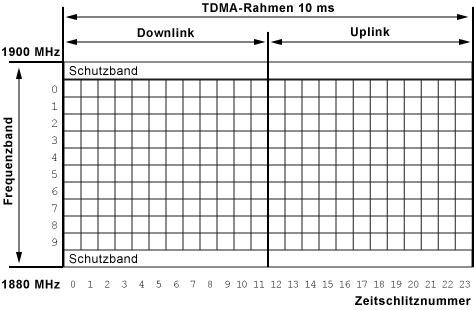
\includegraphics[width=\linewidth]{Kapitel/DECT/Grafiken/frequenzband.png}
\captionof{figure}{Frequenzband von DECT \cite{dect.1}}
\label{fig:dect.frequenzband}
\end{Figure}
Für die Modulation wird das Frequenzband in 10 Frequenzträger unterteilt, jeweils oben und unten befindet sich ein Schutzband, um Störungen durch Überlappungen von anderen Frequenzen zu reduzieren. 

Jeder Frequenzträger wird in 24 Zeitschlitze unterteilt, jeweils 12 Zeitschlitze sind für die Verbindung vom Fixed Part zum Portable Part und umgekehrt reserviert. Die Dauer eines Frames(24 Zeitschlitze) sind 10ms.
Das Nutzsignal wird mit der GFSK Modulation übertragen und bietet eine Bandbreite von 32 kBit/s und bietet damit eine dem Festnetz ähnliche Sprachqualität.

Für die Sprachübertragung werden die Zeitschlitze symmetrisch aufgeteilt, bei Datenübertragungen asymmetrisch mit Bündelung mehrere Kanäle. Bis zu 23 Kanäle lassen sich bündeln, denn es muss nur mindestens ein Kanal für die andere Richtung zur Verfügung stehen \cite{dect.1}.
Die Frequenzmodulation kann allerdings auch mit 4PSK, 8PSK, 16QAM und 64QAM realisiert werden

\subsubsection*{DECT ULE (Ultra-low Energy)}
Bei DECT Ultra-low Energy geht es um die Senkung des Energieverbrauches, die Teilnehmer werden dabei in einen zyklischen Tiefschlaf versetzt. Durch ein Ereignis können die Teilnehmer aus dem Tiefschlaf geholt werden. Kurze Tiefschlafphasen erhöhen allerdings nicht signifikant die Akkulaufzeit, daher wählt man die Pausen möglichst lange, jedoch nicht länger als 20 Sekunden \cite{dect.1}.

\subsubsection*{Datenübertragungen mit DECT}
DECT wurde für die schnurlose Sprachübertragung entwickelt, entsprechend ist DECT zur Datenübertragung nur mit Einschränkungen nutzbar. Mit 24 kBit/s können pro Kanal die Daten übertragen werden. 23 Kanäle lassen sich bündeln, sodass eine Übertragung von 552 kBit/s erreicht werden kann. Üblicherweise können DECT-Datenübertragungsgeräte nur 128 kBit/s übertragen. Mithilfe des DMAP (DECT Multimedia Access Profile) können die vorhandenen 552 kBit/s voll ausgenutzt werden und für ein schurloses Netzwerk auf Basis von DECT verwendet werden. Für die breitbandige Datenübertragung ist dies allerdings nicht ausreichend, weshalb der Nachfolge-Standard CAT-iq entwickelt wurde. \cite{dect.1}

\subsubsection*{GAP - Generic Access Profile}
Das bekannteste DECT-Zugriffsprofil ist das GAP, welches bereits 1994 von ETSI spezifiziert wurde. GAP ermöglicht die Zusammenarbeit zwischen DECT-Geräten unterschiedlicher Hersteller. Alle GAP-kompatiblen Portable Parts lassen sich herstellerunabhängig mit den Telefon-Grundfunktionen an allen GAP-kompatiblen Fixed Parts betreiben. GAP garantiert zwar die Kompatibilität der Mobilteile, jedoch bezieht sich das nur auf die reine Telefonie. Funktionen wie der Anrufbeantworter oder das Telefonbuch funktionieren gegebenenfalls nicht. \cite{dect.4,dect.1}

\subsubsection*{IAP - ISDN Access Networking Profile}
Mithilfe dieser Spezifikation ist ein DECT-Telefon in der Lage ISDN-Komfortmerkmale aus dem Telefonie-Bereich zu nutzen. Zum Beispiel gehört die Rufnummernanzeige, Anklopfen, Dreierkonferenz oder Rufumleitung dazu. Dieses Profil ist weit verbreitet und fast alle DECT-Telefone beherrschen dieses Profil. \cite{dect.1}

\subsubsection*{GIP - GSM Interworking Profile}
Dieses Zugriffsprotokoll regelt die Zusammenarbeit mit digitalen Mobilfunknetzen, die dem GSM-Standard entsprechen (für UMTS existiert auch ein Profil). Mithilfe von Dualmode-Handys lässt sich eine Kombination aus Mobilfunknetz und Festnetz erstellen. Dadurch lässt sich zuhause das Festnetz nutzen und unterwegs das Mobilfunknetz. Unterstützt der Netzbetreiber (Mobilfunk und Festnetz) entsprechende Routing-Techniken, kann für beide Netze dieselbe Telefonnummer angeboten werden. Geräte mit dieser Funktionalität sind jedoch nicht weit verbreitet. \cite{dect.1}
\subsubsection*{DECT CAT-iq}
DECT CAT-iq (Cordless Advanced Technology - internet and quality) soll die Konvergenz von Sprach- und Breitbandübertragungen erhöhen. Neben der Sprachübertragung in Hifi-Qualität können auch Internet-Dienste eingebunden werden. Mithilfe von CAT-iq wird das DECT-Gerät IP-fähig.

Ermöglicht wird damit unter anderem:
\begin{itemize}
\item Musik-Streaming
\item Informationsanzeigen und -dienste aus dem Internet
\item Instant-Messaging 
\item Home-Management-Funktionen
\end{itemize}

Eine Weiterentwicklung von DECT für Datenübertragungen wirkt auf den ersten Blick erst einmal überflüssig. Es stellt sich die Frage warum sollte  etwas neu entwickelt werden, wenn doch die WLAN-Funktechnik genutzt werden könnte zur Übertragung der Daten. Allerdings war WLAN lange nicht als Schnurlostechnik für Telefone geeignet, denn die für die Datenkommunikation ausgelegte WLAN-Technik verbrauchte sehr viel Rechenleistung und hat einen entsprechenden Energieverbrauch. Außerdem funkt WLAN im freien ISM-Band, wo sich auch noch andere Funkanwendungen befinden, weshalb Störungen nicht ausgeschlossen sind. DECT hat den Vorteil ein eigenes Frequenzspektrum zu haben mit einer höheren Reichweite. CAT-iq nutzt den DECT-Frequenzbereich und ist zum bisherigen etablierten DECT-Standard abwärtskompatibel. \cite{dect.3}
\subsection*{Einsatz}
DECT ist als ETSI-Standard für  Kurzstrecken-Funktechnik entwickelt worden und kann für viele Anwendungen in der ganzen Welt in unlizensierten Frequenzbereichen genutzt werden. DECT ist für Telefonie (PSTN und VoIP) und Datenübertragung entwickelt mit einer Reichweite bis zu 500 Metern.

Seit Beginn wurden mehr als 820 Millionen Geräte hergestellt, jährlich kommen ca. 100 Millionen Geräte dazu. DECT dominiert den kabellosen Sprachübertragungssektor mit einem Marktanteil von 73\% von allen kabellosen Technologien (inklusive analogen und proprietären). DECT erhält mehr Marktanteil durch den Austausch von alten analogen Technologien, aber wird verliert auch Marktanteile durch die digitalen Technologien basierend auf IEEE 802.11. Die geringen Kosten von DECT Chipsätzen durch die Massenproduktion erlauben den Austausch von fest verkabelten Telefonen.

DECT wurde initial für Europa entwickelt, ist jedoch mittlerweile in über 110 Ländern adoptiert worden. Die Vereinigten Staaten von Amerika haben sich gegenüber DECT über eine FCC Entscheidung 2005 geöffnet und sind mit der wichtigste Markt hinsichtlich des Wachstums. Japan hat sich vor kurzem auch DECT geöffnet, wo noch traditionell der Markt von The Personal Handy-phone System (PHS) dominiert wird.

Seit 2010 haben viele Betreiber in Europa ihre Telefonnetze auf IP-Netze umgestellt, damit geht eine qualitative Verbesserung der Sprachqualität einher. Statt bisher \SI{3.1}{\kilo\hertz} soll mindestens das Doppelte zur Verfügung stehen. Viele Endgeräte unterstützen  diesen sogenannten HD-Sound bereits.


Neuerungen:
Parallel zur Telefonie können noch weitere Daten übertragen werden, wie z.B. ein externes Adressbuch, Webradio oder ähnliches.
\cite{dect.3,dect.5}
\subsection*{Ausblick}
Innerhalb von Europa sind folgende Frequenzen für DECT reserviert:
\begin{itemize}
\item \SI{1900}-\SI{1920}{\mega\hertz} (geteilt mit UTRAN TDD)
\item \SI{1920}-\SI{1980}{\mega\hertz} (geteilt mit dem Uplink von UTRAN FDD)
\item \SI{2010}-\SI{2025}{\mega\hertz} (vorgesehen für die potentielle Erweiterung von IMT-2000, noch nicht genutzt)
\end{itemize} 

\subsubsection*{Konkurrenz Voice-over-WLAN (VoWLAN)}
WLAN wurde nicht für die Sprachübertragung ausgelegt, jedoch wird mit dem Standard IEEE 802.11e Voice-over-WLAN die Sprachübertragung ermöglicht.

DECT ist für Sprachkommunikation ausgelegt und dank des modularen Aufbaus lassen sich DECT-Netze bei Bedarf mit weiteren Basisstationen erweitern. Durch nahtloses Handover wird eine ständige Konnektivität gewährleistet.

Bei VoWLAN existiert gerade bei Unternehmen in der Regel bereits eine Infrastruktur, weshalb Kosten gespart werden können, da nicht ein weiteres Funknetz aufgebaut werden muss. Allerdings haben DECT Geräte eine längere Akkulaufzeit durch einen geringeren Energieverbrauch als VoWLAN-Geräte.
Letztendlich hängt die Entscheidung zwischen DECT und VoWLAN vor allem von der bestehenden Infrastruktur ab. Wird diese allerdings neu aufgebaut, dann ist es in der Regel günstiger VoWLAN zu nutzen, da keine zwei Infrastrukturen aufgebaut werden müssen. Diese Kostenersparnis wird für viele relevant sein, weshalb DECT eventuell in Zukunft vom Markt verschwinden könnte. WLAN entwickelt sich damit immer mehr zu einer universellen Standard-Infrastruktur. 

Für den Heimanwendungsbereich bietet zum Beispiel die FritzBox in den neueren Modellen mehrere Möglichkeiten. Der DECT Standard ist implementiert, jedoch wird auch eine App für Smartphones zur Verfügung gestellt, mit der man mit seinem Smartphone über WLAN telefonieren kann. 
\cite{dect.6,dect.7,dect.8}
\printbibliography[segment=3,heading=subbibliography]
\end{multicols}

\newpage
\rowcolors{1}{}{}\begin{multicols}{3}[\section{Bluetooth 3.0}]

\rhead{Autor: Johannes Hill}
\lfoot{Letzte Bearbeitung: 16.04.2016}
\newrefsegment

\begin{boxedminipage}{\linewidth}
\begin{tabular}{p{2,1 cm}p{2.7 cm}}
\textbf{Steckbrief}& \\
\end{tabular}
\begin{tabular}{p{1,5 cm}|p{3.3 cm}}
      Einsatz seit & April 2009\\
      \hline
      Frequenz"-bereich  & \SI{2,402}{\giga\hertz}~-~\SI{2,480}{\giga\hertz}\\
      \hline
      Datenrate & \SI{3}{Mbit/s} ohne L2CAP \SI{24}{Mbit/s} mit L2CAP\\
      \hline
      Verbreitung & Weltweit\\
      \hline
      Reichweite & \SI{10}{\metre}~-~\SI{100}{\metre}\\
\end{tabular}
\end{boxedminipage}
\par
%Source http://www.fh-bingen.de/fileadmin/user_upload/Lehrende/Kilsch_Dieter/internet/projekte/TedoSchStiUnits.pdf -> Seite 9 findet ihr alle verwendbaren Einheiten, wie:
%\SI{Zahl}{\mega\hertz} oder \SI{Zahl}{\mili\metre}
%Ich weiß ehrlich gesagt nicht welche Einheiten ihr im Text genau braucht, aber in dem Dokument und mit obigen Beispiel sollte es umsetzbar ein.
\subsection*{Überblick}

\begin{wrapfigure}{r}{0.4\linewidth}
  \vspace{-20pt}
  \begin{center}
  	\hspace{-20pt}
    
\includegraphics[width=0.7\linewidth]{Kapitel/Bluetooth3.0/Grafiken/logo.jpg}
  \end{center}
  \vspace{-15pt}
\end{wrapfigure}

Heutzutage haben elektronische Geräte dank der Miniaturisierung Einzug in das alltägliche Leben gefunden. Mit Bluetooth 3.0, auch bekannt unter dem Code Namen Seattle, können Geräte drahtlos und ohne direkte sichtbare Verbindung miteinander kommunizieren. Darüber hinaus sind die einzelnen Bluetooth Versionen aufgrund von Bluetooth Standard- und Interoperabilitätstest abwärtskompatibel. Das bedeutet, dass Bluetooth 2.1 + EDR Geräte problemlos mit Bluetooth 3.0 Geräten kommunizieren können~\cite{bluetooth3.0.1}. 

Bei der Entwicklung der Bluetooth 3.0 Spezifikation wurde vor allem das Ziel verfolgt, eine wesentliche Steigerung der Datenrate zu realisieren. Sein Vorgänger, sprich Bluetooth 2.1 + EDR, konnte nur eine Datenrate von 3 Mbit/s aufweisen. Damit eine Steigerung der Datenrate verzeichnet werden konnte, war es notwendig eine andere physikalische Schicht zu implementieren. Entsprechende Planungen begannen im Jahr 2006, wobei zwei Ansätze verfolgt wurden: 
\begin{itemize}
	\item Ultra-Wideband  und
	\item IEE 802.11.
\end{itemize} 
Das Ultra-Wideband, das durch die WiMedia Alliance entwickelt wurde, klang anfangs vielversprechend, da es einen geringen Stromverbrauch bei der Byte-Übertragung aufwies. Jedoch war der Stromverbrauch von Ultra-Wideband Controllern zu hoch für mobile Geräte, weshalb dieser Ansatz nicht weiter verfolgt wurde~\cite{bluetooth3.0.2}. 

Die Bluetooth Special Interest Group (SIG) hingegen, legte ihren Fokus den IEEE 802.11. Sie definierte für die Bluetooth 3.0 + HS (High Speed) Spezifikation einen generischen Abstraktions-Layer A2MP (\textbf{A}lternate MAC/PHY \textbf{M}anager \textbf{P}rotocol) für den AMP (\textbf{A}lternate \textbf{M}AC/\textbf{P}HY) und einen 802.11 PAL (\textbf{P}rotocol \textbf{A}dapatation \textbf{L}ayer) für den IEEE 802.11-2007 Standard. Diese Spezifikation ermöglicht zwei Systemvarianten. Bluetooth 3.0 (ohne HS) und Bluetooth 3.0 + HS~\cite{bluetooth3.0.2}.   

\subsection*{Technische Erläuterungen}
Bluetooth verwendet zwei unterschiedliche Kommunikationstypen. Dies ist zum einen die leitungsvermittelte synchrone Kommunikation (SCO) und zum anderen die paketvermittelte asynchrone Kommunikation (ACL). SCO wird nur zur Übertragung von Sprachdaten verwendet. Dementsprechend findet ACL seine Anwendung bei der restlichen Datenübertragung via Bluetooth~\cite{bluetooth3.0.4}.

Bei der Datenübertragung über den Bluetooth Kanal ist die maximale Datenrate auf die Endgeräte, die direkt miteinander kommunizieren, aufgeteilt. Die Datenrate eines Teilnehmers ist daher von folgenden Faktoren abhängig:
\begin{itemize}
	\item Anzahl der Endgeräte, die untereinander gleichzeitig Daten austauschen.
	\item Aktivität anderer Endgeräte.
\end{itemize}
Da Bluetooth das \SI{2,4}{\giga\hertz} Frequenzband nicht alleine verwendet, sondern dieses mit anderen Funktechnologien teilt, sendet Bluetooth nicht mit auf einer festen Frequenz, sondern variiert diese nach jedem Paket. Das angewendete Verfahren wird auch Frequency Hopping Spread Spectrum (FHSS) genannt. Sollte bei der Übertragung eines Pakets über den Kanal ein Fehler auftreten, werden die Daten automatisch erneut übertragen. Weiterhin gilt, dass ein Kanal in sogenannte Zeitschlitze (Slots) der Länge $625\mu$ unterteilt ist~\cite{bluetooth3.0.1}.

Um mehrere Bluetooth Verbindungen (Piconetze) zu garantieren, verwendet jedes Piconetz eine unterschiedliche Hopping-Sequenz. Im \SI{2,4}{\giga\hertz} Frequenzband können 79 Känale angeboten werden~\cite{bluetooth3.0.3}.

\subsubsection*{Klassen und Reichweite}
Bluetooth wurde hauptsächlich für portable Handhelds konzipiert, weshalb der Standard drei verschiedene Sendeleistungen spezifiziert. Entsprechend werden Endgeräte den einzelnen Leistungsklassen zugewiesen. Mobiltelefone sind beispielsweise der Leistungsklasse 3 zugeordnet~\cite{bluetooth3.0.5}. \\

\noindent
\begin{boxedminipage}{\linewidth}
\begin{tabular}{p{1,3cm} | p{1,5cm} | p{1,5cm}}
      \textbf{Klasse} & \textbf{Max. Leistung} & \textbf{Reichweite} \\
      \hline
      Klasse 1 & 100 mW & ca. 100m \\
      \hline
      Klasse 2 & 2,5 mW & ca. 50m \\
      \hline
      Klasse 3 & 1 mW & ca. 10m \\
\end{tabular}
\end{boxedminipage}

\subsubsection*{Piconetze}
Unter einem Piconetz versteht man eine Menge von miteinander kommunizierenden Bluetooth-Geräten. Verknüpft man Piconetze über Bluetooth-Geräte, können diese zu einem sogenannten Scatternetz zusammengefasst werden (siehe Abb. \ref{fig:Piconetze})~\cite{bluetooth3.0.3}.


\begin{Figure}
\begin{center}
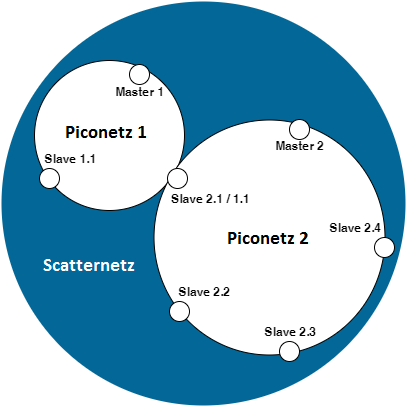
\includegraphics[scale=0.4]{Kapitel/Bluetooth3.0/Grafiken/piconetze.png}
\end{center}

\captionof{figure}{Piconetze und Scatternetze}
\label{fig:Piconetze}
\end{Figure}

\noindent
Piconetze sind aufgeteilt in ein Master- und bis zu sieben Slave Endgeräte. Dabei kann jedes Endgerät Master oder Slave eines Piconetzes sein. Dem Master ist die Aufgabe der Kontrolle des Kanals zugeschrieben, d.h. er entscheidet wer zu welchem Zeitpunkt Datenpakete über den Kanal verschicken darf. Damit dem Slave Endgeräte Senderechte zugewiesen werden kann, schickt ihm der Master ein entsprechendes Datenpaket. Diese Rechte werden dem Slave nach 5 Zeitslots wieder entzogen und der Master entscheidet, ob er ihm diese wieder gewährt. Darüber hinaus kann ein Slave keine weiteren Verbindungen zu anderen Geräten aufbauen, da für ihn nicht absehbar ist, wann Datenpakete vom Master eingehen. Um diese Problematik zu lösen, besteht die Möglichkeit, dass Master und Slave die Rollen tauschen~\cite{bluetooth3.0.1}.

Damit unterschiedliche Piconetze an einem Standort betrieben werden können, kommt das Verfahren des Frequency Hopping zum Einsatz. Dieses berechnet aus der Hardwareadresse des Endgerätes, das eine Verbindung zu anderen Endgeräten aufbauen möchte, die entsprechende Frequency Hopping Sequenz (siehe Abb. \ref{fig:SequenceHopping})~\cite{bluetooth3.0.3}.

\begin{Figure}
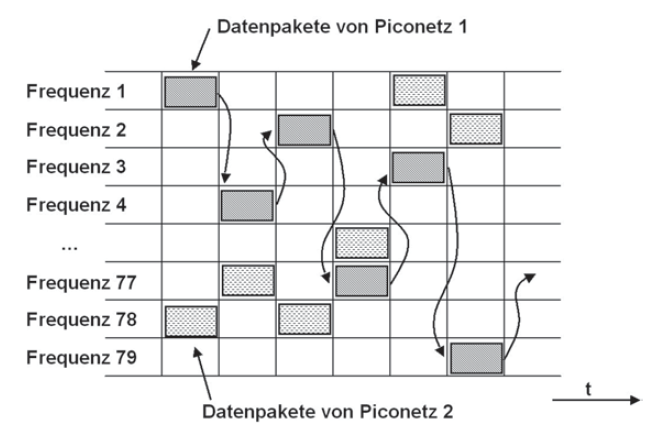
\includegraphics[width=\linewidth]{Kapitel/Bluetooth3.0/Grafiken/frequencehopping.png}
\captionof{figure}{Mehrer Piconetze am gleichen Ort durch Hop-Sequenzen~\cite{bluetooth3.0.1}}
\label{fig:SequenceHopping}
\end{Figure}

\subsubsection*{Der Bluetooth Protokoll Stack}
Grundlage für den Bluetooth Protokoll Stack bildet die ISO-OSI Schichtung (siehe Abb. \ref{fig:ProtokollStack}).Im Folgendem werden die Schichten zwei bis sechs vorgestellt und beschrieben.

\begin{Figure}
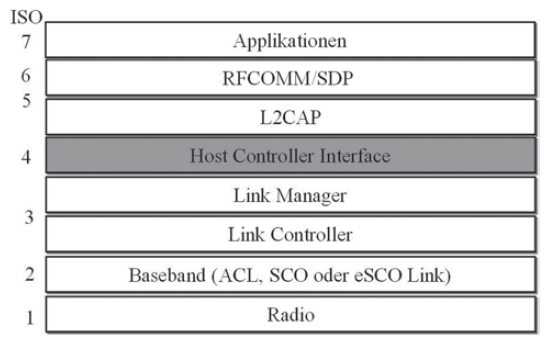
\includegraphics[width=\linewidth]{Kapitel/Bluetooth3.0/Grafiken/Protokoll_Stack.png}
\captionof{figure}{Der Bluetooth Protokoll Stack ~\cite{bluetooth3.0.1}} 
\label{fig:ProtokollStack}
\end{Figure}

\noindent
Der Base Layer übernimmt typische Aufgaben einer Layer 2 Schicht, wie z.B. dem Framing von Datenpaketen. Entsprechende Frametypen wurden bereits unter den Kürzeln SCO und ACL vorgestellt~\cite{bluetooth3.0.1}. 

Für den Aufbau, Erhalt und den korrekten Abbau von Verbindungen ist der Link Controller \hspace{1px} zuständig. Zu \hspace{1px} seinen \hspace{1px} weiteren \hspace{1px} Aufgaben zählen das Steuern der Funkkanäle, Frequenzwechsel und Funkverbindungen, sowie die Fehlerkorrektur (Forward Error Correction FEC) bei der Datenübertragung~\cite{bluetooth3.0.3}.

\end{multicols}
\newpage
\section*{Historische Entwicklung}
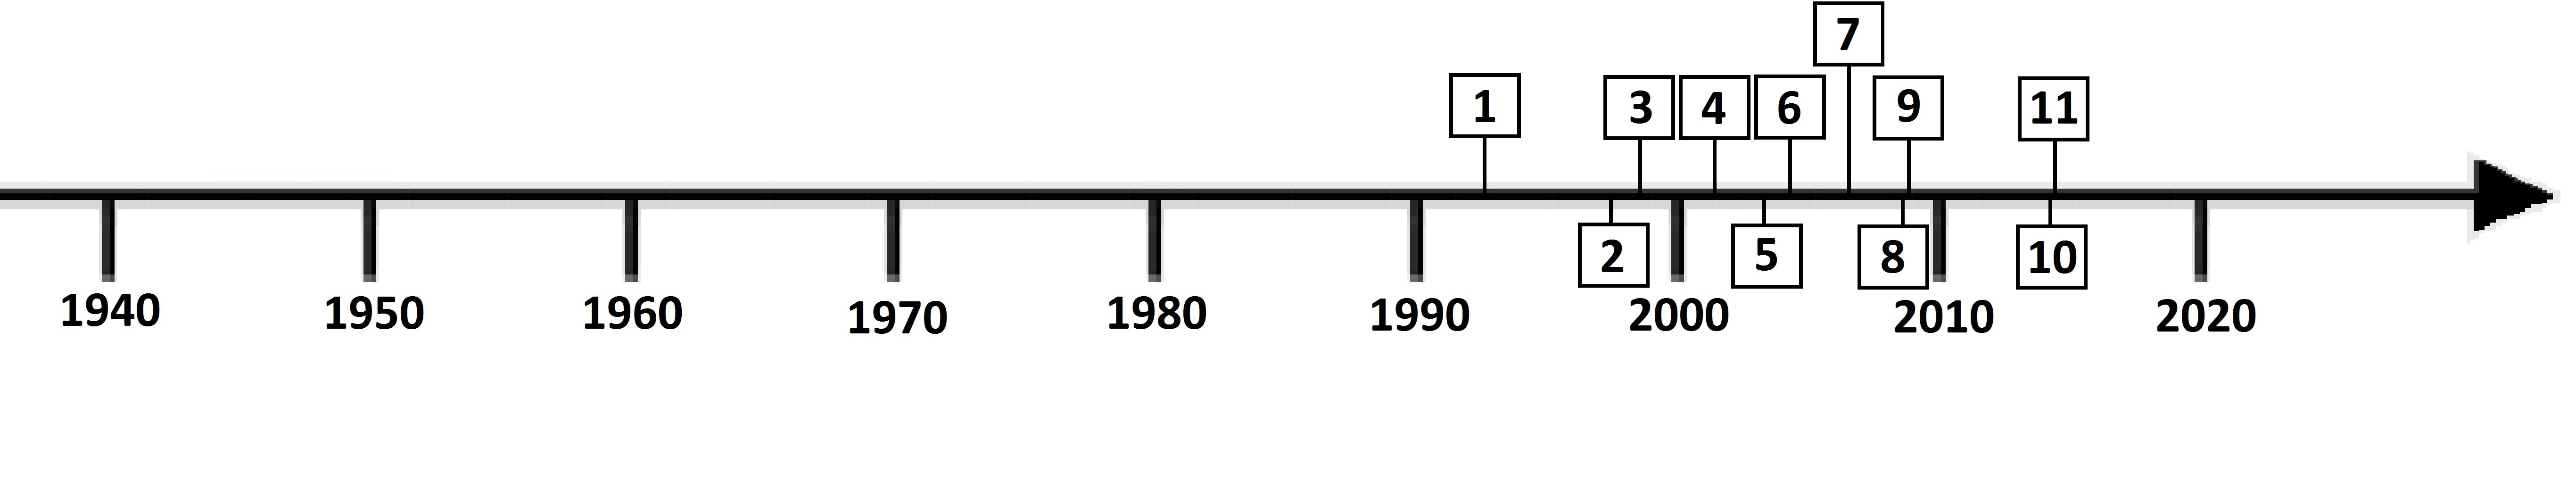
\includegraphics[width=\textwidth]{Kapitel/Bluetooth3.0/Grafiken/Zeitstrahl}
\par
\noindent

\vspace{-0.3cm}
\begin{tabular}{|p{1 cm}|p{3 cm}|p{13.55 cm}|}
	\hline
	Nummer & Datum & Information \\
	\hline
	1 & August 1993 & Gründung der Infrared Data Association (IrDA) mit dem Ziel ein einheitliches Protokoll für Datenübertragung über Infrarot bereitzustellen.\\
	\hline
	2 & 1998 & Gründung der Bluetooth Special Interest Group (SIG) durch die Firmen Ericsson, Nokia, IBM, Toshiba und Intel zur Ausarbeitung eines Standards, der verbindliche Spezifikationen festlegte.\\
	\hline
	3 & Juli 1999 & Bereitstellung der Spezifikation Bluetooth 1.0 (Juli) und Bluetooth 1.0b (Dezember).\\
	\hline
	4 & Februar 2001 & Bereitstellung der Spezifikation Bluetooth 1.1.\\
	\hline
	5 & November 2003 & Bereitstellung der Spezifikation Bluetooth 1.2.\\
	\hline
	6 & November 2004 & Bereitstellung der Spezifikation Bluetooth 2.0 + EDR.\\
	\hline
	7 & August 2007 & Bereitstellung der Spezifikation Bluetooth 2.1 + EDR.\\
	\hline
	\textbf{8} & \textbf{April 2009} & \textbf{Bereitstellung der Spezifikation Bluetooth 3.0 + HS}.\\
	\hline
	9 & Dezember 2009 & Bereitstellung der Spezifikation Bluetooth 4.0.\\
	\hline
	10 & Dezember 2013 & Bereitstellung der Spezifikation Bluetooth 4.1.\\
	\hline
	11 & Dezember 2014 & Bereitstellung der Spezifikation Bluetooth 4.2.\\
	\hline
\end{tabular}
\begin{multicols}{3}

Der Link Manager ist für die Einrichtung und Aufrechterhaltung von Verbindungen zuständig. Dazu wird das Link Manager Protocol (LMP) eingesetzt, welches ebenfalls Sicherheit, Identifikation und Verbindungskontrolle garantieren soll~\cite{bluetooth3.0.3}.

Mit dem Host Controller Interface (HCI) verfolgt man das Ziel, Endgeräte und Bluetooth Chip physikalisch voneinander zu trennen. Zu seiner Aufgabe zählt es, Daten und Kommandos für den Link Manager in definierten Kommandos und Nachrichtenpaketen zwischen Endgerät und Bluetooth Chip (Controller) zu übertragen~\cite{bluetooth3.0.1}.

Das Logical Link Control und Adaption Protocol (L2CAP) unterscheidet Protokolle von höheren Ebenen (z.B. RFCOMM, BNEP und SDP) und kann mehrere Verbindungen zu einem Gerät über eine physikalische ACL Verbindung multiplexen (siehe Abb. \ref{fig:l2cap}). Durch die Erweiterung des L2CAP in der Bluetooth Spezifikation 3.0 war es nun möglich den High Speed Kanal zu nutzen~\cite{bluetooth3.0.1}.

\begin{Figure}
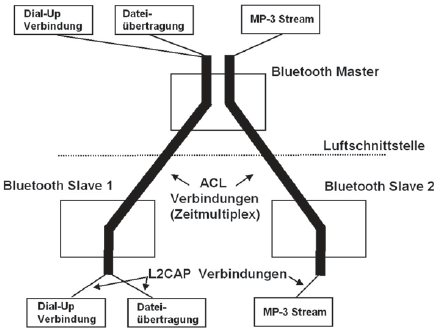
\includegraphics[width=\linewidth]{Kapitel/Bluetooth3.0/Grafiken/l2cap.png}
\captionof{figure}{Der Bluetooth Protokoll Stack~\cite{bluetooth3.0.1}}
\label{fig:l2cap}
\end{Figure} 

\noindent
Abschließend sollen das Service Discovery Protocol (SDP) und die Radio Frequency Comport Emulation (RFCOMM) betrachtet werden. SDP hat die Funktion, die für Anwendungen zur Verfügung stehenden Dienste ausfindig zu machen. RFCOMM hingegen stellt virtuelle serielle Schnittstellen für Dienste zur Verfügung und vereinfacht diesen dadurch die Datenübertragung ~\cite{bluetooth3.0.3}.

\subsubsection*{Bluetooth 3.0 Erneuerungen}
Mit der Bluetooth Spezifikation 3.0 wurde das Enhanced Power Control für ein effizienteres Energiemanagement eingeführt. Weiterhin implementierte man den High Speed (HS) Modus, der für den Verbindungsaufbau Bluetooth verwendet und für die Datenübertragung den Wi-Fi Kanal nutzt~\cite{bluetooth3.0.1}.

Die technische Umsetzung sah vor, den BR/EDR (\textbf{B}asic \textbf{R}ate/\textbf{E}nhanced \textbf{D}ata \textbf{R}ate) Controller von Bluetooth 1.X/2.X um einen oder mehrere AMP (Alternate MAC/PHY) und einen ULP (Ultra Low Power) Controller zu erweitern. Damit sind vier Transceiver in dieser Spezifikation vorzufinden~\cite{bluetooth3.0.2}.

Mit A2MP ermöglichte man, dass der AMP Manager nach anderen AMP Managern in remote Geräten suchen kann. Dieser verwaltet Abfrageinformationen, physikalische Links und ist für die Erzeugung spezifischer AMP Schlüssel zuständig~\cite{bluetooth3.0.2}.

Auch der L2CAP Layer wurde erweitert, indem eine verbesserte Flow Spezifikation, eine erweiterte Window Size und der Enhanced Retransmission Mode implementiert wurde~\cite{bluetooth3.0.2}. 

\subsection*{Einsatz}
In foglenden Anwendungsfällen kommt diese Technologie zum Einsatz:~\cite{bluetooth3.0.1}:
\begin{itemize}
	\item Kabellose Verbindungen zwischen einem Smartphone und Audiogeräten wie z.B. Kopfhörer. 
	\item Austausch von Daten zwischen Endgeräten.
	\item Anbindung von kabellosen Eingabegeräten wie z.B. Tastaturen.
\end{itemize}

\subsection*{Anbieter und Gremien}
Im Jahr 1994 began Ericsson die ersten Untersuchungen bzgl. kabelloser Geräteverbindungen. 4 Jahre später gründeten sie gemeinsam mit IBM, Intel, Nokia und Toshiba die Bluetooth Special Interest Group (SIG). Heute gehören mehr als 8000 Unternehmen zu dieser Interessengemeinschaft, die an der Entwicklung neuer Bluetooth Spezifikationen beteiligt sind~\cite{bluetooth3.0.5}.

\subsection*{Ausblick}
Die in diesem Artikel vorgestellte Bluetooth Spezifikation wurde noch im gleichen Jahr durch seinen Nachfolger abgelöst. Bluetooth 4.0 integrierte eine Low Energie Option, indem Wibree in den Bluetooth Standard mit aufgenommen wurde~\cite{bluetooth3.0.1}. 

In Bluetooth 4.1 legte man den Fokus auf die Entwicklung einer Verbindung, die sich nach einer Signalunterbrechung automatisch wieder aufbauen konnte. Dies ist die letzte Erweiterung am Bluetooth Standard, die durch die SIG eingeführt wurde~\cite{bluetooth3.0.1}. Weitere technische Erweiterungen sind zu erwarten. 

\printbibliography[segment=4,heading=subbibliography]

\end{multicols}
\newpage
\rowcolors{1}{}{}\begin{multicols}{3}[\section{Bluetooth 4.0}]

\rhead{Autor: Thomas Schaffroth}
\lfoot{Letzte Bearbeitung: 17.04.2016}

\newrefsegment

\begin{boxedminipage}{\linewidth}
\begin{tabular}{p{2,1 cm}p{2.7 cm}}
\textbf{Steckbrief}& \\
\end{tabular}
\begin{tabular}{p{2,1 cm}|p{2.7 cm}}
      Einsatz seit & Juni 2010\\
      \hline
      Frequenz"-bereich  & \SI{2400}{\giga\hertz}\\
      \hline
      Datenrate & \SI{1}{MBit/s}\\
      \hline
      Verbreitung & Weltweit\\
      \hline
      Reichweite & \SI{10}{\metre}\\
\end{tabular}
\end{boxedminipage}
\par
%Source http://www.fh-bingen.de/fileadmin/user_upload/Lehrende/Kilsch_Dieter/internet/projekte/TedoSchStiUnits.pdf -> Seite 9 findet ihr alle verwendbaren Einheiten, wie:
%\SI{Zahl}{\mega\hertz} oder \SI{Zahl}{\mili\metre}
%Ich weiß ehrlich gesagt nicht welche Einheiten ihr im Text genau braucht, aber in dem Dokument und mit obigen Beispiel sollte es umsetzbar ein.
\subsection*{Überblick}
Die Bluetooth Technologie wurde im Jahr 1994 als drahtlose Alternative zu Datenkabeln entwickelt, indem man Daten über Funk übertrug. Bluetooth wurde als offener Standard entworfen, um Verbindungen und Zusammenspiel zwischen verschiedenen Produkten und Industrien möglich zu machen.\cite{Bluetooth_4.1} Beispiele für die Nutzung von Bluetooth im Alltag sind Freisprechanlagen für Smartphones im Auto, das Telefonieren über Bluetooth Headsets, das Hören von Musik über einen drahtlosen Lautsprecher oder die Übertragung von Daten zwischen zwei mobilen Geräten, uvm. In diesem Artikel werden zu Beginn die Architektur, das Übertragungsverfahren und die Rahmenstruktur von Bluetooth allgemein erläutert, da sich daran in der Spezifikation 4.0 nichts geändert hat. Anschließend wird auf die Neuerungen von Bluetooth 4.0 eingegangen.

\subsection*{Technische Erläuterungen}
\subsubsection*{Architektur der Bluetooth Technologie}
Die Verbindung zwischen Bluetooth Geräten erfolgt über ein Piconetz. Ein Piconetz ist ein Personal Area Network von Endgeräten, die sich über Bluetooth verbunden haben. Unter einem Personal Area Network versteht man ein Netz, das von Kleingeräten wie PDAs (Personal Digital Assistant) oder Mobiltelefonen ad hoc auf- und abgebaut werden kann. 

Ein Piconetz besteht aus einem Master-Knoten, bis zu sieben aktiven Slave-Knoten, die sich in einem maximalen Umkreis von 10 m befinden, und bis zu 255 geparkten Knoten. Dabei entspricht ein Knoten einem mobilen Gerät bzw. Teilnehmer. Geparkte Knoten sind Geräte, die der Master in einen Ruhezustand versetzt hat, um den Batterieverbrauch zu senken. In diesem Zustand wird ein Gerät nur durch eine Aktivierung des Masters wieder aktiv gesetzt. Darüber hinaus ist es möglich mehrere Piconetze über einen Bridge-Knoten zu verbinden. Es entsteht ein sog. Scatternetz (Abbildung 1). In einem Piconetz sind Slaves nicht eigenständig sondern warten auf Anweisungen durch den Master. Dieser steuert den Takt und entscheidet wer in welcher Zeitscheibe (Zeitintervall) Daten übertragen darf. Die Kommunikation geschieht dabei nie von Slave zu Slave sondern  immer über den Master-Knoten.\cite{Bluetooth_4.2}

\begin{Figure}
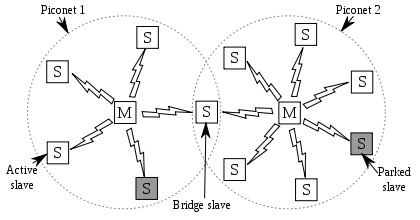
\includegraphics[width=\linewidth]{Kapitel/Bluetooth_4/Grafiken/piconetz.png}
\captionof{figure}{Zwei Piconetze druch einen Bridge-Knoten zu einem Scatternetz verbunden       \cite{Bluetooth_4.3} }
\label{fig:vorlage.vorlesungssaal}
\end{Figure}

\subsubsection*{Übertragungsverfahren}
Die Übertragung von Daten erfolgt über die Funkschicht. Bluetooth benutzt dafür das ISM-Band (Industrial, Scientific, Medical) im 2,4 GHz-Bereich. Daraus ergeben sich 79 Kanäle mit je einem MHz Bandbreite. Da jedoch das ISM-Band auch von anderen Netzen verwendet wird, kann es zu Störungen kommen. Um dies zu verhindern, wird bei Bluetooth eine Frequenzsprungtechnik mit Spektrumsspreizung verwendet. Es können bis zu 1600 Sprünge in der Sekunde über Zeitscheiben mit einer Dauer von 625 Mikrosekunden geschehen. In einem Piconetz springen alle Knoten zur gleichen Zeit und richten sich nach der Zeitscheibenvorgabe und Sprungfolge des Masters. Dazu kommt, dass sich Übertragungen früherer Versionen von Bluetooth und IEEE 802.11-Übertagungen gegenseitig zerstörten (Abbildung 2). Aus diesem Grund wurde die Frequenzsprungfolge so verändert, dass sie Kanäle auf denen andere Radio Frequenz-Signale existieren auslassen, um die schädlichen Interferenzen zu verkleinern. Diese Methode wird als adaptives Frequenzsprungverfahren (Abbildung 3) bezeichnet.\cite{Bluetooth_4.2}

\begin{Figure}
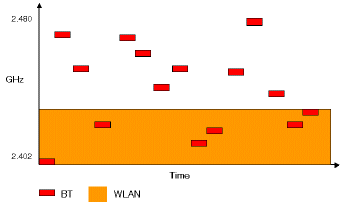
\includegraphics[width=\linewidth]{Kapitel/Bluetooth_4/Grafiken/kollisionen.png}
\captionof{figure}{Überlagerungen zwischen Bluetooth und IEEE 802.11\cite{Bluetooth_4.5} }
\label{fig:vorlage.vorlesungssaal}
\end{Figure}

\begin{Figure}
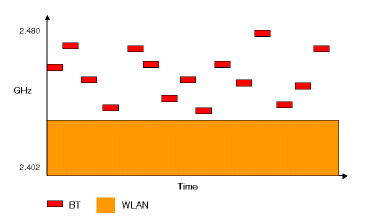
\includegraphics[width=\linewidth]{Kapitel/Bluetooth_4/Grafiken/frequenzsprung.png}
\captionof{figure}{Lösung durch das adaptive Frequenzsprungverfahren\cite{Bluetooth_4.5} }
\label{fig:vorlage.vorlesungssaal}
\end{Figure}

\subsubsection*{Rahmenstruktur}
Unter "Rahmen" versteht man in diesem Umfeld den Protokollrahmen, d.h. den Aufbau der Pakete, die zwischen Bluetooth Geräten ausgetauscht werden. Zwei wichtige Rahmenformate von Bluetooth sind in Abbildung 4 dargestellt, es gibt aber noch verschiedene andere. Den Anfang eines Rahmens bildet ein Zugriffscode, der den Master bestimmt. Dadurch können Slaves in der Reichweite von zwei Master-Knoten ermitteln, welche Daten für sie bestimmt sind. Es folgt ein 54-Bit-Header mit denselben Feldern, die auch für die MAC-Teilschicht im OSI-Modell typisch sind. 

Widmen wir uns kurz dem Header. Das Address-Feld gibt an, für welches Gerät im Piconetz der Rahmen bestimmt ist. Das Feld Type  spezifiziert den Rahmentyp (z.B. Polling), die Anzahl der Zeitscheiben, die der Rahmen umfasst, und die Art der Fehlerkorrektur, die im Datenfeld angewendet wird. Als nächstes stehen drei Flags. Das Flow-Bit kann von einem Slave-Knoten gesetzt werden, um anzuzeigen, dass sein Speicher voll ist, er also keine Daten mehr empfangen kann. Das Acknowledgement-Bit dient der Mitsendung einer Bestätigung in einem Rahmen. Das Sequence-Bit wird zur Nummerierung von Rahmen verwendet, um redundante Übertragungen zu erkennen. Schließlich folgt eine Prüfsumme von 8 Bit. 

Wenn der Rahmen mit Basisdatenrate gesendet wird, folgen auf den Header die Daten. Das Datenfeld kann abhängig davon über wie viele Zeitscheiben die Übertragung stattfindet von 0-2744 Bit lang sein. In dem Fall, dass der Rahmen mit erweiterter Datenrate gesendet wird, kann das Datenfeld bis zu zwei- oder dreimal so viele Bits besitzen. Den Daten ist nun ein Sicherheitsfeld und Synchronisationsmuster vorangestellt. Die Aufgabe des Synchronisationsmusters ist es, auf die schnellere Datenrate umzuschalten. Der Grund ist, dass der Adresscode und der Header mit Basisrate und nur die Daten mit erweiterter Datenrate gesendet werden. Üblicherweise werden Rahmen mit erweiterter Datenrate mit einem Trailer abgeschlossen.\cite{Bluetooth_4.2}

\begin{Figure}
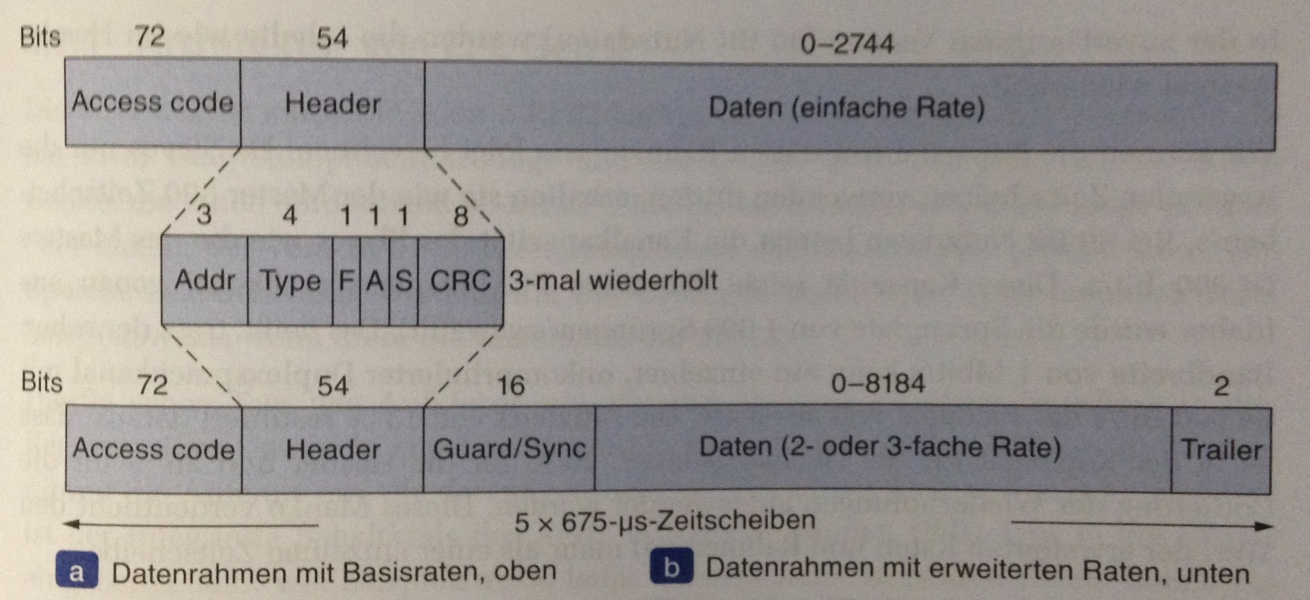
\includegraphics[width=\linewidth]{Kapitel/Bluetooth_4/Grafiken/rahmenstruktur.jpg}
\captionof{figure}{Überblick über die Rahmenstruktur in Bluetooth\cite{Bluetooth_4.2}
}
\label{fig:vorlage.vorlesungssaal}
\end{Figure}

\end{multicols}
\newpage
\section*{Historische Entwicklung}
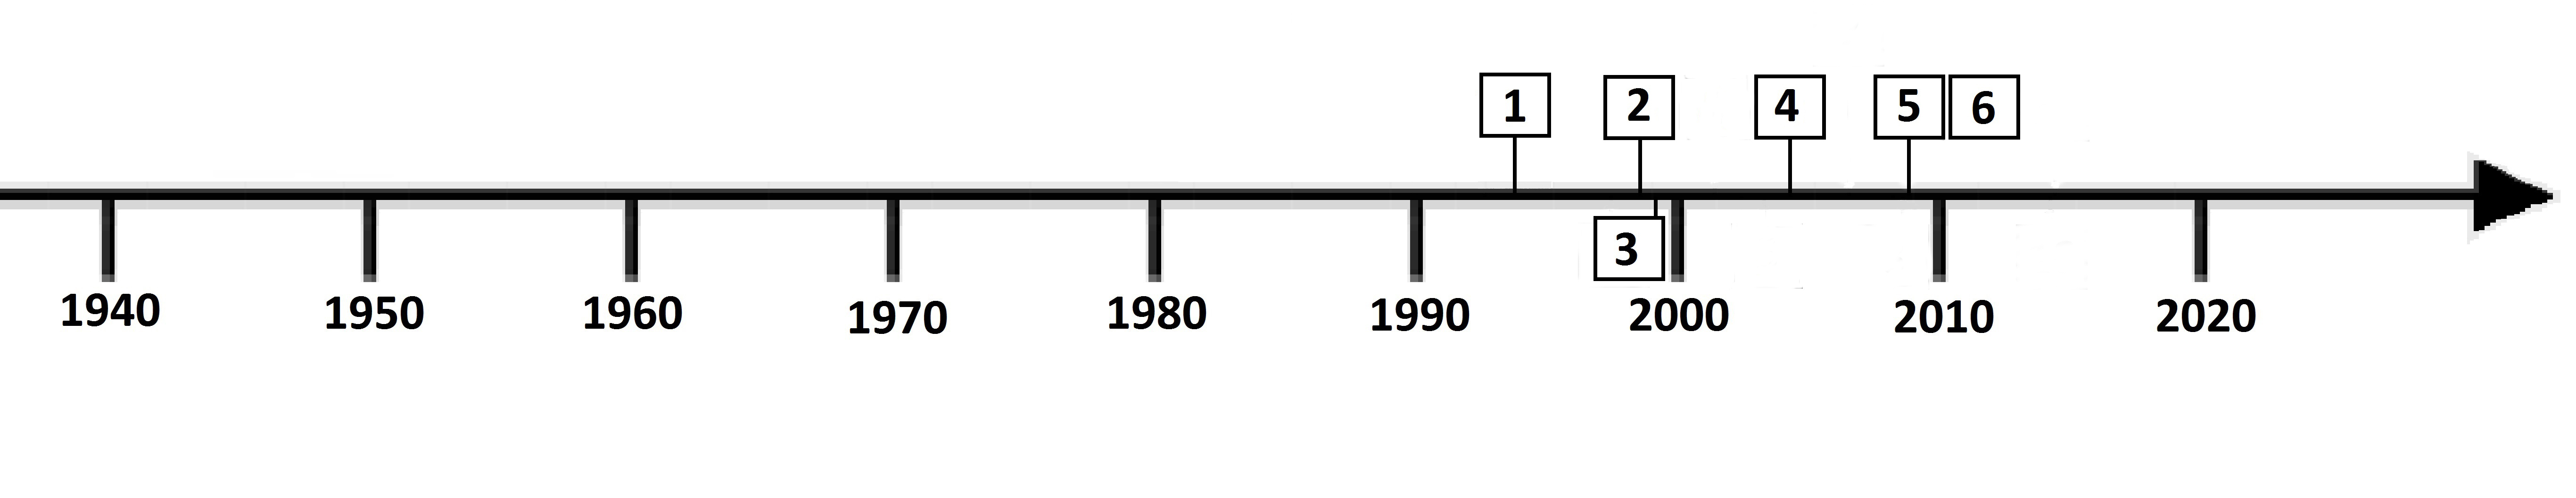
\includegraphics[width=\textwidth]{Kapitel/Bluetooth_4/Grafiken/zeitstrahl_bearbeitet}
\par
\noindent
\begin{tabular}{|p{1 cm}|p{3 cm}|p{13.55 cm}|}
	\hline
	Nummer & Datum & Entwicklungsschritte~\cite{Bluetooth_4.2}\\
	\hline
	1 & 1994 & Das Unternehmen L.M.Ericsson beginnt mit der Entwicklung einer Technologie für kabellose Verbindungen zwischen Mobiltelefonen und anderen Geräten.\\
	\hline
	2 & 1998 & Bildung der Bluetooth Special Interest Group (SIG) mit vier anderen Unternehmen, um einen drahtlosen Standard zur Verbindung von Rechnern und Kommunikationsgeräten zu spezifizieren. Die Prämisse dafür ware kostengünstige Funktgeräte mit niedrigem Strombedarf zu verwenden.\\
	\hline
	3 & Juli 1999 & Veröffentlichung von Bluetooth 1.0\\
	\hline
	4 & 2004 & Nachdem die Protokolle aus Version 1.0 stabil laufen werden diese mit höheren Datenraten zu Bluetooth 2.0 ergänzt.\\
	\hline
	5 & 2009 & Mit der dritten Version von Bluetooth werden in Kombination mit IEEE 802.11 Datenübertragungen mit höherem Durchsatz möglich\\
	\hline
	5 & Dezember 2009 & Veröffentlichung der Spezifikation für Bluetooth 4.0, die Niedrigenergiebetrieb inkludiert\\
	\hline
\end{tabular}
\par
\begin{multicols}{3}

\subsubsection*{Neuerungen von Bluetooth 4.0}
Man spricht bei Bluetooth in der Version 4.0 auch von Bluetooth Low Energie (LE). Der Name leitet sich davon ab, dass es sich um eine im Gegensatz zu seinen Vorgängern sehr stromsparende Version handelt. Dadurch ergeben sich nun auch Anwendungsmöglichkeiten auf Geräten bei denen dies bisher nicht möglich gewesen wäre, da einfach die Batterie für den längeren Betrieb von Bluetooth nicht ausgereicht hätte. Für die Chips von Bluetooth 4.0 reicht nur eine kleine Batterie aus, um längere Zeit arbeiten zu können. Low-Energy-Geräte ab Bluetooth 4.0 sind speziell für Anwendungen ausgelegt, die in größeren Intervallen kleine Datenmengen übertragen. Reine Low-Energy-Geräte sind beispielsweise Smartwatches, Sportsensoren oder Aktivitätstracker, die sich mit einem Smartphone koppeln. Bluetooth 4.0 ist allerdings nur bedingt zu früheren Versionen kompatibel. Ein Gerät, dass nur Bluetooth 4.x kennt, setzt bei seiner Gegenstelle ebenfalls Bluetooth 4.x voraus.\cite{Bluetooth_4.6}

\subsection*{Einsatz}
Die Bluetooth SIG spezifiziert Anwendungen, die unterstützt werden sollen und stellt für jede eine Reihe von Protokollen bereit. Es existieren eine ganze Reihe von Anwendungen auch „Profile“ genannt. Im Folgenden werden zunächst ausgewählte Profile und ihre Anwendungen vorgestellt, die nicht mit Bluetooth 4.0 spezifiziert wurden, sondern mit älteren Versionen. Diese wurden jedoch in der 4.0-Spezifikation übernommen und mit neuen Profilen ergänzt. Einige Profile sind für die Übertragung von Audio und Video vorgesehen. Ein Beispiel ist das Interkommunikationsprofil (ICP, INTP), welches es möglich macht zwei Telefone als Walkie-Talkies zu verbinden. Dazu kommen Headset- und Freisprechprofile, um Peripheriegeräte wie Headsets mit einer Basisstation zu verbinden. Andere Profile regeln das Streamen von Audio- und Videodaten in Stereoqualität beispielsweise von einem Handy auf einen tragbaren Lautsprecher oder von einer Kamera auf einen Fernseher. 

Außerdem existieren Profile zum Verbinden von Tastaturen und Mäusen an einen PC (HID), um ein Handy als Fernbedienung für einen Bluetooth-fähigen Fernseher zu verwenden oder Profile, die Netzbetrieb ermöglichen. Zu letzteren gehören zum Beispiel das PAN-Profil (Personal Area Networking) mit dem Bluetooth-Geräte ein Ad-hoch-Netz bilden können oder das DUN-Profil (Dial-Up Networking) durch das sich ein Notebook kabellos mit einem Handy verbinden kann, dass ein Modem enthält. Erwähnenswert ist das Generic-Attribute-Profil (GATT), dass für die neue Version Bluetooth 4.0 spezifiziert wurde. Es wird als Master-Profil für andere Profile verwendet, um kleine Datenmengen energieeffizient zu übertragen. \cite{Bluetooth_4.2} Eine vollständige Übersicht aller bisherigen Profile inklusive GATT mit ihren Einsatzgebieten kann hier gefunden werden: https://de.wikipedia.org/wiki/Bluetooth-Profile.

\subsection*{Anbieter und Gremien}
Für die Bluetooth-Technologie einschließlich der Version 4.0 ist die Bluetooth SIG (Special Interest Group) zuständig. Diese wurde 1998 von 5 Unternehmen gegründet und war im März 2015 bereits eine Interessengemeinschaft von mehr als 8000 Unternehmen, die bei der Entwicklung und Verbreitung der Technologie zusammenwirken. Die Bluetooth SIG ist darüber hinaus auch der Eigentümer des Bluetooth-Zeichens und Herausgeber der Bluetooth-Spezifikation.\cite{Bluetooth_4.4}

\subsection*{Ausblick}
Die Bluetooth-Technologie ist heute für das kabellose 
Verbinden von verschiedenen Geräten unerlässlich geworden. 
Das gilt sowohl für die älteren Spezifikationen als auch für 
Bluetooth 4.0 durch das völlig neue Einsatzgebiete möglich werden. 
Dies betrifft vor Allem den Betrieb auf kleinen Geräten für die 
Bluetooth-Anwendungen bisher aufgrund des hohen Energieverbrauchs
nur bedingt nützlich waren. Meiner Meinung nach ist die Technologie
von Bluetooth sehr interessant und es ist lohnenswert sich damit einmal
genauer zu befassen zumal fast jeder von uns Bluetooth schon benutzt hat. 
Darüber hinaus bleibt es spannend zu verfolgen inwiefern sich Bluetooth 4.0 
und seine Einsatzgebiete in den nächsten Jahren entwickeln werden.
\printbibliography[segment=3,heading=subbibliography]
\end{multicols}

\newpage

\rowcolors{1}{}{}\begin{multicols}{3}[\section{Iridium}]

\rhead{Benita Rojewski}
\lfoot{08.05.2016}

\newrefsegment

\begin{tabular}{p{2,1 cm}p{2.7 cm}}
\textbf{Steckbrief}& \\
\end{tabular}
\rowcolors{1}{\topicolor!20}{}
\begin{tabular}{p{2,1 cm}p{2.7 cm}}
      Einsatz seit & September 1998\\
      Vorwahl & +8816 und +8817\\
      Frequenz"-bereich  & L-Band:
      \SI{1616}bis\SI{1626.5}{\mega\hertz}, 
      K-Band: \SI{19.4} bis\SI{19.6} {\giga\hertz}, \SI{29.1} bis \SI{29.3} {\giga\hertz}\\
      Datenrate (komprimiert) & \SI{26} bis \SI{27} {bit/s}\\
      Datenrate (unkomprimiert) & \SI{2.4} bis \SI{2.5} {bit/s}\\
      Verbreitung & Weltweit, Iridium Satellite and Network Operations Center \\
      Modulation & FDMA, TDMA\\
      Sendeleistung (während des Sendens) & max. 7 Watt\\
      Sendeleistung (während des Empfangs) & 0.6 Watt\\
      Verschlüsselung/ Kodierung & „Advanced Multi-Band Excitation“ (AMBE)\\
      Schutzart & IP54\\
      Dual Play & Ja\\
      Triple Play & Nein\\
\end{tabular}
\par
%Source http://www.fh-bingen.de/fileadmin/user_upload/Lehrende/Kilsch_Dieter/internet/projekte/TedoSchStiUnits.pdf -> Seite 9 findet ihr alle verwendbaren Einheiten, wie:
%\SI{Zahl}{\mega\hertz} oder \SI{Zahl}{\mili\metre}
%Ich weiß ehrlich gesagt nicht welche Einheiten ihr im Text genau braucht, aber in dem Dokument und mit obigen Beispiel sollte es umsetzbar ein.
\subsection*{Überblick}

In der Kommunikationstechnik ist Iridium der Name für ein drahtloses Kommunikationsnetz. Dieses besteht aus 68 Satelliten, von denen zwei Reserve sind. Sie befinden sich in einer Höhe von  780 km in sechs nahezu polaren Umlaufbahnen mit je elf sich im aktiven Einsatz befindenden Satelliten und einem Reservesatelliten je Bahn. Somit liegen diese in erdnaher Umlaufbahn. Dadurch ist es gewährleistet, dass Signale von einem Mobiltelefon gesendet und empfangen werden können (siehe Abb. \ref{fig:sv}).
Da ursprünglich dieses System aus 77 Satelliten bestehen sollte, hat es den Namen Iridium erhalten. Dieses Element hat im Periodensystem die Ordnungszahl 77.\cite{I3,I5}

\begin{Figure}
	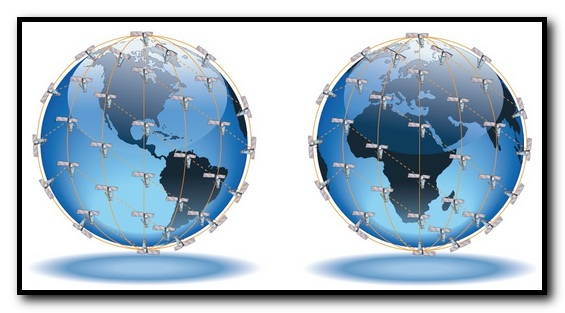
\includegraphics[width=\linewidth]{Kapitel/Iridium/Grafiken/satellitenverteilung.jpg}
	\captionof{figure}{Satellitenverteilung~\cite{I6}}
	\label{fig:sv}
\end{Figure}


\subsection*{Technische Erläuterung}
Die Verknüpfung der Iridium-Satelliten ist netzförmig und mit den Iridium-Gateways weltweit verbunden. Erst dadurch entsteht die Möglichkeit,mit den öffentlichen Telefon- und Mobil-funknetzen in Kontakt zu treten.
Zudem sind die Satelliten des Iridium-Netzwerks untereinander durch Intersatellitenlinks verbunden. 

Eine aktive Verbindung kommt zustande, wenn sich ein Satellit in Reichweite einer Vermittlungsstelle auf der Erdoberfläche befindet. Dadurch entsteht der Weg in das uns bekannte Telefonnetz. Besteht keine Verbindung von den Satelliten zur Empfangsstation, so werden die Telefongespräche oder auch Signale über andere Iridium-Satelliten weitergeleitet, bis es zu einer Kontaktaufnahme mit einem Empfangssatelliten kommt.

Im \textbf{L}(ong)-Band werden die Daten vom Satelliten zum Endgerät übertragen. Die Übertragung zwischen den Satelliten und von diesen zur Empfangsstation erfolgt im \textbf{Ka}(y-ay)-Band. In Abbildung \ref{fig:Fs} ist das Frequenzspektrum des Iridium-Systems mit der jeweiligen Aufgabe dargestellt: 

\begin{Figure}
	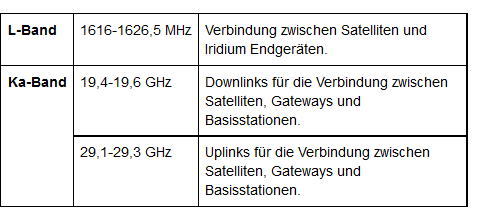
\includegraphics[width=\linewidth]{Kapitel/Iridium/Grafiken/band.png}
	\captionof{figure}{Frequenzspektrum des Iridium-Systems~\cite{I1}}
	\label{fig:Fs}
\end{Figure}

Kommunizieren zwei Iridium-Nutzer  miteinander, so wird dieses Gespräch direkt zwischen den Satelliten vermittelt, ohne eine Erdstation dazwischen zu schalten. ~\cite{I1, I4}



\subsubsection*{Netzabdeckung}
Voraussetzung für die Iridium-Kommunikation ist eine klare Sicht zum Himmel in alle Richtungen ab einem Höhenwinkel von 8.2 Grad. Befindet sich jedoch ein Objekt ab diesem Winkel am Himmel, so wird die Kommunikation gestört bzw. unterbrochen. Deshalb wird als Maßstab hierfür die geballte Faust bei waagrecht ausgestrecktem Arm verwendet. Diese Höhe entspricht ungefähr diesem Höhenwinkel. Damit ergibt sich folgende  Netzabdeckung unter dem Höhenwinkel von 8.2 Grad (siehe Abb. \ref{na8.2}).

In Gegenden, in denen tiefe Schluchten oder Bergtäler sind, kann es häufig zu Verbindungsunterbrechungen kommen, so dass es sein kann, dass erst 120 Minuten später wieder eine Verbindung zustande kommt. Grund hierfür ist, dass in diesen zwei Stunden kein Iridium- Satellit in Sichtkontakt kommt.
Die Abbildung \ref{na21} zeigt die Netzabdeckung unter dem Höhenwinkel von 21 Grad in tiefen Schluchten 
\begin{Figure}
	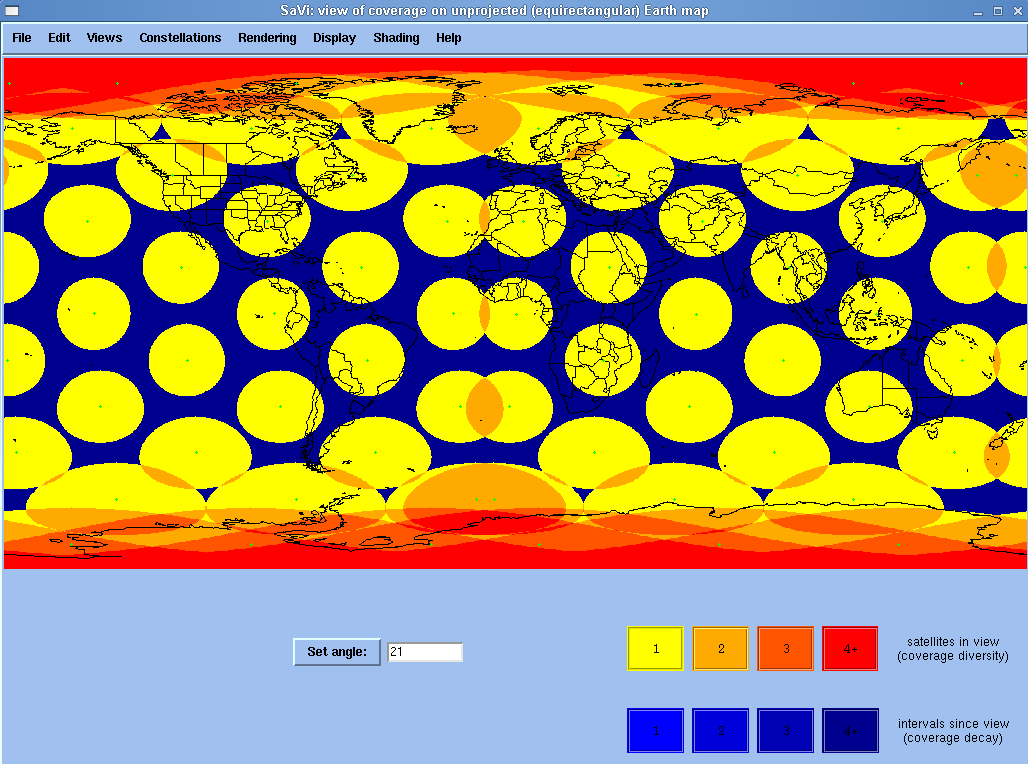
\includegraphics[width=\linewidth]{Kapitel/Iridium/Grafiken/netzabdeckung21.png}
	\captionof{figure}{Netzabdeckung unter dem Höhenwinkel von 21 Grad in tiefen Schluchten ~\cite{I4}}
	\label{na21}
\end{Figure}

Mit Hilfe von Iridium- Satelliten ist es auch möglich, die Polregionen abzudecken. Der Grund hierfür liegt darin, dass auch auf der polaren Umlaufbahn Satelliten platziert sind, so dass dort die Versorgungsdichte besonders hoch ist, da eine geringere freie Sicht zum Himmel als am Äquator benötigt wird.

\begin{Figure}
	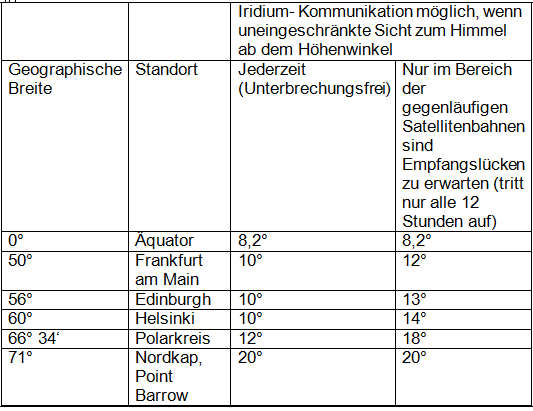
\includegraphics[width=\linewidth]{Kapitel/Iridium/Grafiken/hoehenwinkel.png}
	\captionof{figure}{Höhenwinkel~\cite{I4}}
	\label{fig:hw}
\end{Figure}

Im Durchschnitt findet alle neun Minuten während eines Telefonats ein automatischer Wechsel der Iridium-Satelliten statt, da der verwendetet Satellit hinter dem Horizont verschwindet. Diesen Wechsel bemerken die Gesprächsteilnehmer nur, wenn der alte Satellit hinter dem Horizont verschwindet und der neue Satellit noch nicht in Sichtweite ist.~\cite{I4}

\subsection*{Einsatz}
Vorteil von Iridium ist die Erreichbarkeit in Bereichen mit wenigen Basisstationen, schlechter Verbindung, in freier Natur und in unwegsamen Gelände, die so gut wie immer gegeben ist.
Einige Bereiche, in denen diese Technologie angewendet wird: 

\begin{itemize}
	\item SMS
	\item Militär
	\item Paging
	\item Email
	\item Gas- und Ölgesellschaften
	\item Baugesellschaften
	\end{itemize}

Allerdings kann es auch vorkommen, dass die Frequenzen belegt sind oder die dortige Regierung die Verwendung von Iridium nicht genehmigt, wodurch dann die Kommunikation eingeschränkt ist. Seit 2015 besteht dieses Problem z.B. in den Ländern Kuba und Nordkorea. In Russland und Indien dagegen ist der Import, Export und die Verwendung von Iridium-Satelliten erlaubt, allerdings besteht eine Meldepflicht für solche Art von Telefonen.~\cite{I3,I4}

\subsection*{Anbieter und Gremien}

Für die Satellitensteuerung und die Netzverwaltung ist das \textit{Iridium \textbf{S}atellite and \textbf{N}etwork \textbf{O}perations \textbf{C}enter} (SNOC) zuständig. Ihr Sitz ist im Norden des US-Bundesstaates Virginia. Zudem gibt es Kontrollstellen, die für Telemetrie und Funkpeilung (TTAC) zuständig sind. Diese befinden sich auf Hawaii und in Kanada.

Es kommt durch die Kooperation von vielen nationalen und internationalen Mobilfunknetzen zu Roaming-Partnern, weswegen der Iridium-Kunde über diese seine Telefongespräche führt und damit verschiedene Netze, wie z.B. GSM, AMPS und CDMA, weltweit zu nutzen. Befinden sich die Kunden außerhalb der Versorgungsbereiche der lokalen Mobilfunknetze, so kommen die Satellitennetze zum Einsatz. ~\cite{I1}



\end{multicols}
\newpage
\section*{Historische Entwicklung}
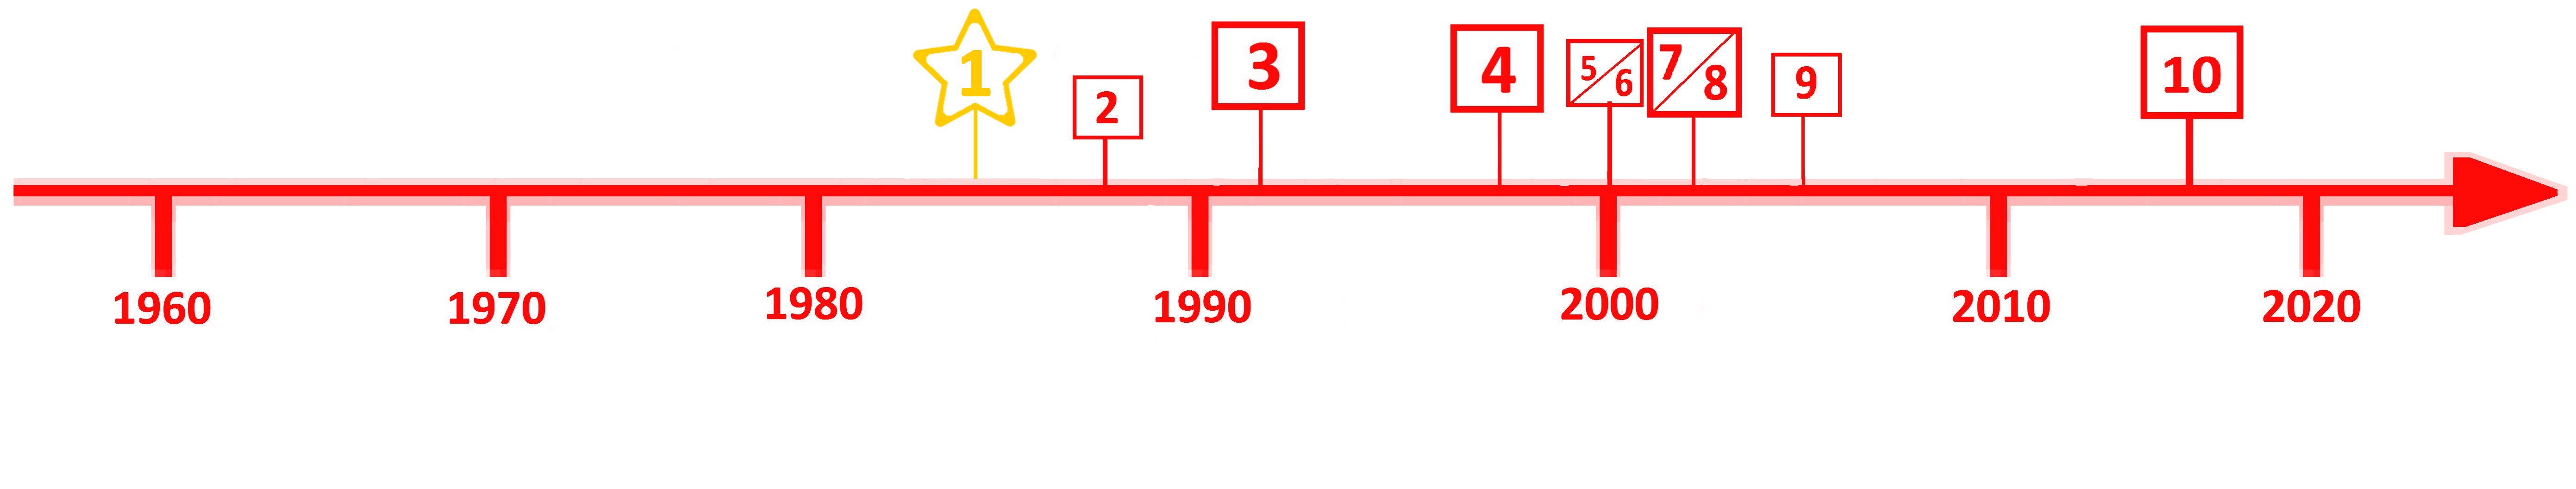
\includegraphics[width=\textwidth]{Kapitel/Iridium/Grafiken/Zeitstrahl_Iridium_rot}
\par
\noindent
\rowcolors{2}{}{\topicolor!20}
\begin{tabular}{p{0.5 cm}p{1.5 cm}p{15.55 cm}}
	Nr. & Datum & Entwicklungsschritte~\cite{I2},~\cite{I4}\\
	1 & 1985 & Geburt der Idee für Iridium bei \textit{Motorola}. Es sollte die weltweite Sprach- und Datenübermittlung über Satellitentelefon und \textbf{PDA}s (\textbf{P}ersonal \textbf{D}igital \textbf{A}ssistant) ermöglichen.\\
	2 & bis 1988 & Konzeptentwurf\\
	3 & 1991 & Gründung des Unternehmens \textit{Iridium Inc}.\\
	4 & 1998  & In Betriebnahme des Systems 
	\\
	5& März 2000 & geplante Abschaltung, allerdings wurde diese auf Grund des Druckes der Öffentlichkeit zum Teil verschoben.\\
	6 & 23.08.2000 & Konkursanmeldung des Unternehmens\\
	7 & 01.01.2001 & Übernahme des neugegründeten Unternehmens \textit{Satellite LLCt}, Betriebnahmen und Wartung der Satelliten von \textit{Boening}, Hersteller ziviler und militärischer Flugzeuge und Hubschrauber sowie von Militär- und Weltraumtechnik\\
	8 & 30.03.2001 & Wiederaufnahme des kommerziellen Betriebes\\
	9 & 2005 & deutliche Senkung der Gerätepreise und Telefonatkosten\\
	10 & ab 2017 & Iridium-NEXT- Satelliten mit ADS-B- Empfänger ermöglichen die Flugzeugkontrolle in Regionen\\
	
\end{tabular}
\par
\begin{multicols}{3}

\subsubsection*{Preise und Endgeräte}
Durch das Iridiumsystem ist es möglich geworden, weltweit, ob auf dem Land, auf dem Wasser oder in der Luft, miteinander zu kommunizieren. Die Kosten eines Iridium-Telefonats wurden 2001 und 2005 gesenkt, so dass sich diese zwischen 0.90 und 1.50 US-Dollar pro Minute belaufen.

Ein mögliches Endgerät ist das Iridium Telefon (Beispielmodell: Iridium 9555). Dieses ist sowohl im Mobilfunk- als auch im Satellitennetz nutzbar, so dass der Kunde den Zugriff auf beide Netze hat.

Ein anderes Endgerät ist der sogenannte Iridium-Pager. Dieser kann alphanumerische Nachrichten empfangen. Da dieser den internationalen Zeichensatz erkennt, ist das Gerät weltweit verwendbar. Durch eine Batterie es einen Monat funktionsfähig.~\cite{I1, I4}

\subsection*{Ausblick}
Die zweite Generation von Iridium-Satelliten heißt "Iridium Next". Hierzu wurden 81 neue Satelliten bestellt, von denen ab 2015 72 in die Umlaufbahn gebracht werden sollten.  Allerdings wurde der Start des Einsatzes der ersten beiden Iridium-Next-Satelliten wegen technischer Probleme auf April 2016 verschoben. Diese Satelliten sollen zudem abwärtskompatibel sein. Eine weitere Neuheit bei dieser Generation ist die Nutzung von IP-basierten Datenübertragungen, wodurch es auch möglich sein soll, dass sowohl auf See als auch in den Polarregionen zuverlässigerer Empfang ist.~\cite{I2, I7}


\printbibliography[segment=13,heading=subbibliography]
\end{multicols}
\begin{Figure}
	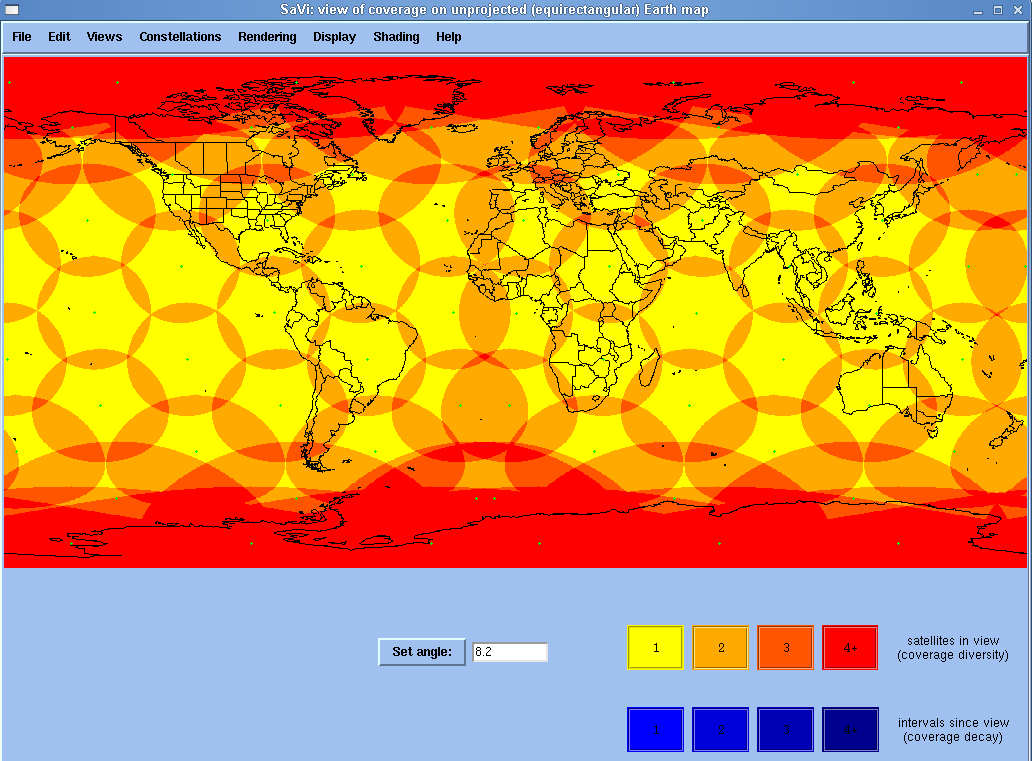
\includegraphics[width=\linewidth, height= 7.6 cm]{Kapitel/Iridium/Grafiken/netzabdeckung82.png}
	\captionof{figure}{Netzabdeckung unter dem Höhenwinkel von 8.2 Grad~\cite{I4}}
	\label{na8.2}
\end{Figure}

\newpage

\rowcolors{1}{}{}\begin{multicols}{3}[\section {D-Netz}]

\rhead{Autor: Tizian Kurkamp}
\lfoot{Letzte Bearbeitung: 15.04.2016}

\newrefsegment

\begin{boxedminipage}{\linewidth}
\begin{tabular}{p{2,1 cm}p{2.7 cm}}
\textbf{Steckbrief}& \\
\end{tabular}
\begin{tabular}{p{2,1 cm}|p{2.7 cm}}
      Einsatz seit & 1992\\
      \hline
      Frequenz"-bereich  & \SI{890} - \SI{960}{\mega\hertz}\\
      \hline
      Modulationsart & GMSK\\
      \hline
      Bandbreite eines Kanals & \SI{200}{\kilo\hertz}\\
      \hline
      Sendeleistung der Basisstation & <\SI{50}{\watt}\\
      \hline
      Sendeleistung im Endgerät & Handy:  \SI{2}{\watt}, "Auto bis \SI{14}{\watt}\\
\end{tabular}
\end{boxedminipage}
\par
%Source http://www.fh-bingen.de/fileadmin/user_upload/Lehrende/Kilsch_Dieter/internet/projekte/TedoSchStiUnits.pdf -> Seite 9 findet ihr alle verwendbaren Einheiten, wie:
%\SI{Zahl}{\mega\hertz} oder \SI{Zahl}{\mili\metre}
%Ich weiß ehrlich gesagt nicht welche Einheiten ihr im Text genau braucht, aber in dem Dokument und mit obigen Beispiel sollte es umsetzbar ein.

\subsection*{Überblick}


Das D-Netz ist ein zellulares Mobilfunknetz nach dem GSM-Standard. Die Namensgebung durch den Buchstaben D erfolgt in Fortsetzung der bisherigen Buchstabenbezeichnung für die Funknetze.
Das D-Netz ist digitalisiert, sowohl was die Wählvermittlung (Signalling) anbelangt als auch für Übertragung von Daten und Sprache. Letztere werden quantisiert, digitalisiert und pulscodemoduliert, wodurch sie störungsarm und regenerierbar sind und somit auch unter schwierigen Bedingungen übertragen werden können. Besonderes Kennzeichen dieses Zellularnetzes ist das automatische Handover und das automatische Auffinden von Teilnehmern, deren Standort nicht bekannt ist, selbst dann, wenn derzeit kein Gespräch geführt wird und keine Datenverbindung besteht.

Unter dem Namen D-Netz (oder auch DNetz) werden gleich zwei Netze zusammengefasst. Sowohl die Telekom (D1) als auch Vodafone nutzen D-Netz Frequenzen um ihre Mobilfunk-Dienste abzuwickeln. Das D-Netz stand ursprünglich für ein digitales Netz im GSM-900-Frequenzbereich und wurde dann später durch das E-Netz (genutzt von E-Plus und O2) erweitert. Die Namen D1-Netz (für das Netz der Telekom bzw. T-Mobile) und D2-Netz (für das Netz von Vodafone) leiten sich noch aus der ursprünglichen Aufteilung ab.
Mittlerweile gibt es mit UMTS-Netze und LTE Netzen deutlich mehr Mobilfunk-Netze, die genutzt werden können, die Bezeichnungen haben sich aber mittlerweile so eingebürgert, dass auch ohne die eigentliche Netz-Grundlage viele Nutzer diese Kennungen verwenden.


\subsection*{Technische Erläuterungen}

Die Übertragung findet im 900-MHz-Bereich statt, und zwar in den Teilbereichen 890 MHz bis 915 MHz und 935 MHz bis 960 MHz. Der untere Frequenzbereich wird für die Übertragung vom Mobilfunk-Sender/Empfänger zur Basisstation benutzt (Uplink), der obere für die entgegengesetzte Richtung (Downlink). Die Mobilstation wird mit Handy bezeichnet und hat eine Sendeleistung von 0,8 W bis 5 W. Die jeweils 25 MHz breiten Frequenzbereiche, sind in 124 Kanäle unterteilt, von denen jeder 200 kHz breit ist Zur Modulation wird das Gaussian Minimum Shift Keying (= GMSK) verwendet. 

\begin{Figure}
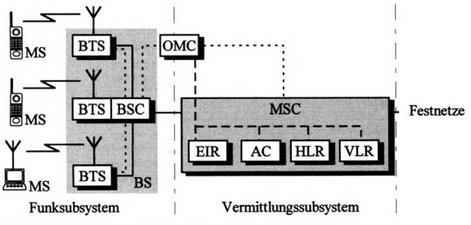
\includegraphics[width=\linewidth]{Kapitel/DNetz/Grafiken/systemaufbau.png}
\captionof{figure}{Systemaufbau des D-Netzes~\cite{DNetz.2}}
\label{fig:DNetz.systemaufbau}
\end{Figure}

Entsprechend der Abbildung \ref{fig:DNetz.systemaufbau} besteht das D-Netz aus der 

\begin{itemize}
	\item Mobilen Station (MS) \\
	Die im Allgemeinen ein Funktelefongerät darstellt. Es kann sich aber prinzipiell um jedes D-Netz-kompatibles Endgerät handeln, 		 	z.B. einen Laptop mit Sende und Empfangseinheit.
	\item Basis Station (BS)
	unterteilt in
		\begin{itemize}
			\item Base Transceiver Station (BTS)
			als reinem Funksende- und Empfangsteil
			\item Base Station Controller (BSC)
			als Steuerungsteil
		\end{itemize}
	\item Funkvermittlung (Mobile Service Switching Center = MSC) mit je einer 
		\begin{itemize}
			\item Besucherdatei (Visitor location Register = VLR)
			\item Heimatdatei (Home Location Register = HLR)
			\item Authentifizierungszentrale (Authentification Center = AC)
			\item Endgerätkennungsdatei (Equipment Identity Register = EIR)
		\end{itemize}
	\item Zentralen Betriebstechnik (Operation and Maintenance Center = OMC)
\end{itemize}






\subsection*{Anbieter}

Für das D-Netz gibt es zwei Betreiber: Die Telekom mit dem D1-Netz und Vodafone mit dem D2-Netz. Da beide Netze nach dem GSM-Standard betrieben werden, gibt es technisch kaum Unterschiede. Damit man die beiden Betreiber an den Rufnummern unterscheiden kann, sind die Netzkennzahlen unterschiedlich.

Anbieter im D1-Netz  (Telekom)

\begin{itemize}
\item chixx
\item congstar
\item Deutsche Telekom
\item freenetmobile
\item ja!mobil
\item Lebara
\item Penny Mobil
\item sparhandy
\item turkcell
\end{itemize}

Anbieter im D2-Netz (Vodafon)

\begin{itemize}
\item 1und1
\item BILDmobil
\item callmobile.de
\item discotel
\item EDEKA Mobil
\item EWE
\item FYVE
\item klarmobil
\item mobilcom debitel
\item otelo
\item Rossmann mobil
\item smartmobil
\item Vodafone
\end{itemize}
(Vgl. ~\cite{DNetz.1})



\end{multicols}
\newpage
\section*{Historische Entwicklung}
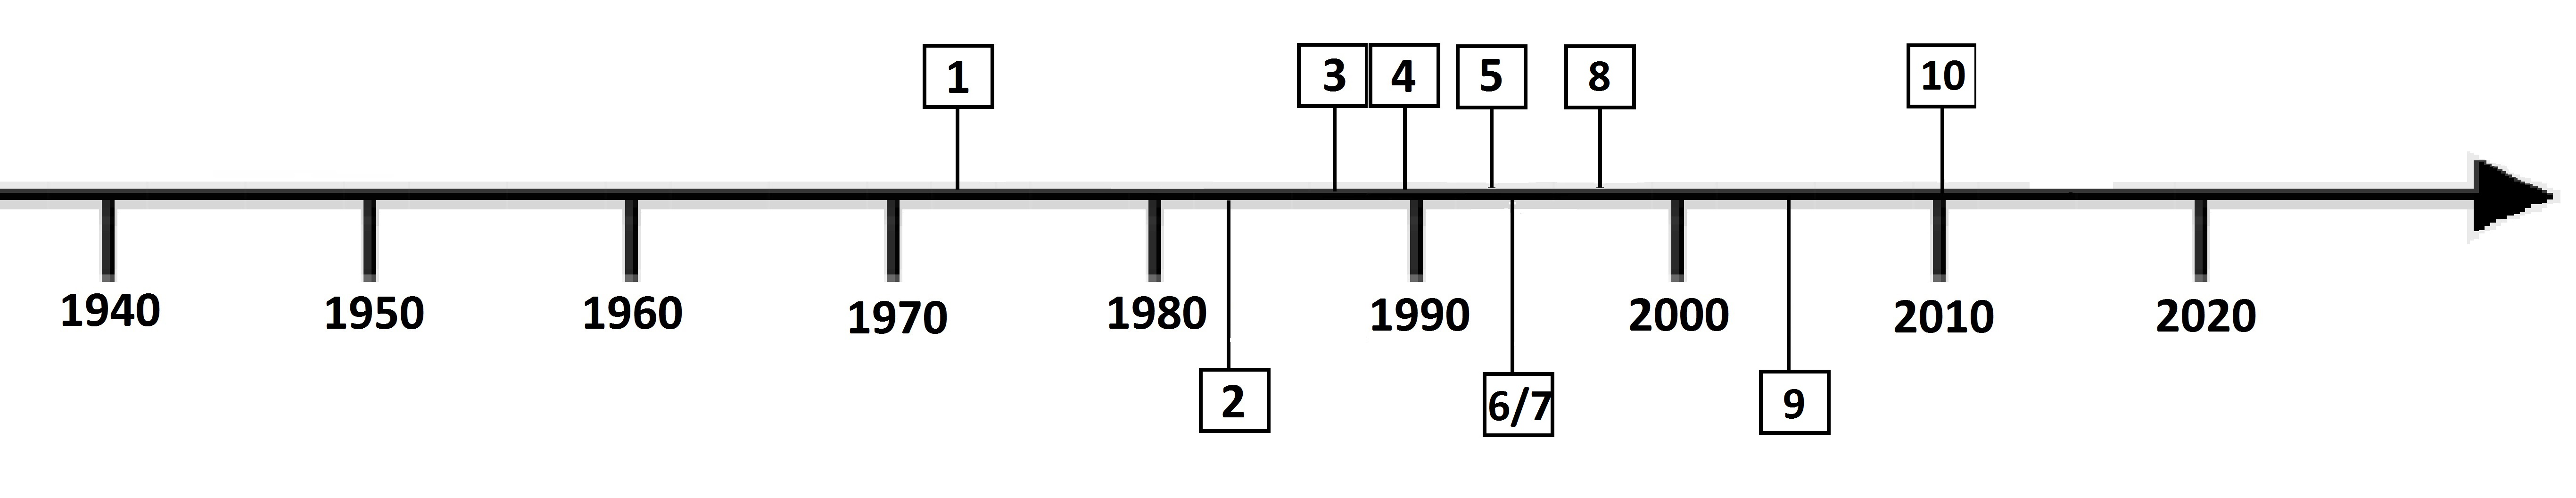
\includegraphics[width=\textwidth]{Kapitel/DNetz/Grafiken/Zeitstrahl}
\par
\noindent
\begin{tabular}{|p{1 cm}|p{3 cm}|p{13.55 cm}|}
	\hline
	Nummer & Datum & Entwicklungsschritte~\cite{DNetz.3}\\
	\hline
	1 & 1972 & Realisierung des B-Netzes\\
	\hline
	2 & 1982 & Gründung der Groupe Speciale Mobile (GSM)\\
	\hline
	3 & 1986 & Einführung des C-Netzes\\
	\hline
	4 & 7. Dezember 1989 & Vergabe einer Lizenz an ein Konsortium unter der Führung des Mannesmann-Konzerns\\
	\hline
	5 & 1. Juli 1992 & Start des Regelbetriebs des D- Netzes\\
	\hline
	6 & April 1993 & ca. 130.000 Netz-Teilnehmer bei der Telekom\\
	\hline
	7 & Ende 1993 & 80ige Abdeckung Deutschlands durch das D2-Netz\\
	\hline
	8 & 1994/95 &  Einführung des E-Plus-Mobilfunknetzes\\
	\hline
	9  & 2004 &  ca. 71 Millionen Mobilfunknutzer und Einführung des UMTS-Netzes\\
	\hline
	10 & 2010 & Einführung des LTE-Mobilfunkstandards\\
	\hline
\end{tabular}
\par
\begin{multicols}{3}

1982 wurde die Groupe Speciale Mobile gegründet, die für Europa ein einheitliches digitales Mobilfunksystem entwickeln sollte. Als sich Ende der 1980er Jahre die praktische Umsetzung des Standards abzeichnete, wurde in Deutschland vom Postminister Christian Schwarz-Schilling entschieden, dass neben der Bundespost auch ein privater Anbieter eine Lizenz für den Betrieb eines Netzes des GSM-Standards erhalten sollte. In dem Ausschreibungsverfahren wurde festgelegt, dass zwischen beiden Betreibern faire Wettbewerbsbedingungen bestehen sollten. Insgesamt zehn Firmen bewarben sich um die Lizenz, die am 7. Dezember 1989 schließlich an ein Konsortium unter Führung des Mannesmann-Konzerns vergeben wurde, das nach Meinung des Lenkungsausschusses Mobilfunk den leistungsfähigsten Bewerber darstellte.
Nach einer einjährigen Versuchsphase wurde der Regelbetrieb am 1. Juli 1992 gestartet. Als unmittelbarer Nachfolger des C-Netzes erhielt das neue Netz die Bezeichnung „D-Netz“.
Das D1-Netz ist das Netz der Deutschen Telekom, während das D2-Netz das Mobilfunknetz der Firma Vodafon bezeichnet, ehemals Mannesmann Mobilfunk. Nach der Einführung des E-Plus-Mobilfunknetzes 1994 setzte ein erheblicher Preisfall bei den Endgeräten, sowie bei der Tarifstruktur ein, sodass die Teilnehmerzahl rapide stieg.(Vgl. ~\cite{DNetz.3} und ~\cite{DNetz.4})

\subsection*{Ausblick}

Als das Handy sich in den 1990er-Jahren in Deutschland etablierte, war Mobilfunk noch etwas Besonderes und die Nutzung von Handys vorwiegend auf das Telefonieren und SMS-Schreiben beschränkt. Auch die Netzabdeckung steckte in Deutschland noch in den Kinderschuhen. Heute gehört das Smartphone mit seinen vielseitigen Funktionen zum Standard des modernen Menschen. Mobil Surfen, Telefonieren, Chatten oder Bilder versenden ist dank moderner Mobilfunknetze problemlos auch unterwegs möglich. Vor allem der neue Standard LTE verspricht Internetgeschwindigkeiten, wie man sie bisher nur von DSL im Heimbereich gewohnt war.
Die vier großen Mobilfunkbetreiber, die Telekom, o2, Vodafone und E-Plus kommen in Deutschland auf eine nahezu vollständige GSM-Netzabdeckung. Somit sollten Sie mit jedem Anbieter fast überall in Deutschland problemlos telefonieren oder eine Kurznachricht versenden können. In Deutschland haben wir also im GSM-Netz eine Netzabdeckung von nahezu 100 Prozent! Allerdings zeigt es sich in der Praxis des Öfteren, dass in manchen Gebieten beim Telefonieren Funklöcher entstehen. Außerdem gibt es noch Unterschiede in der Netzabdeckung mit den verschiedenen Übertragungsarten wie UMTS oder LTE.

Schnelle Übertragungsraten sind theoretisch auch heute schon per LTE Advanced möglich. Die zukünftige Entwicklung der Mobilfunkstandards wird demnach nicht allein von der bereits erreichten Bandbreite, sondern noch viel stärker davon abhängen, wie gut die Netze ausgebaut werden, damit auch das gesamte Leistungsspektrum genutzt werden kann.

Ein wichtiger Motor für den Ausbau der Mobilfunkstandards ist u.a. auch der Mobile Commerce als Teil des E-Commerce. Denn immer mehr Menschen kaufen auch mit ihrem Tablet oder Smartphone im Internet ein. Durch den flächendeckenden Ausbau des LTE-Netzes ist es dann auch möglich, überall und jederzeit in Deutschland online einzukaufen. Auch die Internetnutzung allgemein wird LTE verändern, denn bei voller Netzabdeckung wäre niemand mehr in Deutschland auf einen Festnetzanschluss angewiesen, um schnelles Internet zu nutzen. Vielleicht werden dann in Zukunft auch Festnetzanschlüsse obsolet?

LTE ist zukunftsweisend, der Netzausbau des mobilen Internets wird voraussichtlich den Ausbau des DSL-Netzes in Deutschland übertreffen. Für Bewohner in ländlichen Regionen wäre dies zukünftig eine gute Nachricht, denn sie sind bis dato immer noch vom schnellen Breitbandinternet abgeschnitten.


\printbibliography[segment=5,heading=subbibliography]
\end{multicols}
\newpage

\rowcolors{1}{}{}\begin{multicols}{3}[\section{C-Netz}]

\rhead{Autor: Daniel Keilmann}
\lfoot{Letzte Bearbeitung: 16.04.2016}

\newrefsegment

\begin{boxedminipage}{\linewidth}
\begin{tabular}{p{2,1 cm}p{2.7 cm}}
\textbf{Steckbrief}& \\
\end{tabular}
\begin{tabular}{p{2,1 cm}|p{2.7 cm}}
      Einsatz seit & 01.05.1985\\
      \hline
      Funkkanäle & 287 (ab 1991)\\
      \hline
      Verbreitung & DE, PT und ZA\\
      \hline
      Auslastung & 850.000 Teilnehmer\\
      \hline
      Eingestellt & 31.12.2000\\
\end{tabular}
\end{boxedminipage}
\par

\subsection*{Überblick}
Das C-Netz der DeTeMobil war seit Mitte 1984 verfügbar und startete offiziell im September 1985. Ende 2000 wurde der Betrieb eingestellt. \enquote{Anders als beim B-Netz betrieben die Nachbarländer Netze mit einem anderen technischen Standard, sodass die deutsche Form des C-Netzes nur noch in Portugal und Südafrika genutzt wurde.}~\cite{c-netz.1}\\
Zu dem Thema C-Netz wird auf die folgenden Aspekte eingegangen:
\begin{itemize}
	\item Technische Erläuterung
	\begin{itemize}[label={}]
		\item In diesem Abschnitt wird die technische Umsetzung des C-Netzes untersucht.
	\end{itemize}	
	\item Vergleich zum A- und B-Netz 
	\begin{itemize}[label={}]
		\item Hier werden die technischen Unterschiede von dem C-Netz zum A- und B-Netz dargelegt.
	\end{itemize}
	\item Einsatz		
	\begin{itemize}[label={}]
		\item Wo das C-Netz verwendet wird und wieweit es von den Bürgern benutzt wird.
	\end{itemize}
	\item Anbieter und Gremien
	\begin{itemize}[label={}]
		\item Wer das C-Netz zur Verfügung stellt.
	\end{itemize}
	\item Historische Entwicklung
	\begin{itemize}[label={}]
		\item Entwicklung des C-Netzes.
	\end{itemize}
	\item Ausblick
	\begin{itemize}[label={}]
		\item Was noch mit dem C-Netz realisiert wird und welche Folgetechnologien eingesetzt wurden.
	\end{itemize}
\end{itemize}
\subsection*{Technische Erläuterungen}

\begin{boxedminipage}{\linewidth}
\begin{tabular}{p{2,1 cm}p{2.7 cm}}
\textbf{Frequenzbereich}~\cite{c-netz.1} & \\
\end{tabular}
\begin{tabular}{p{2,1 cm}|p{2.7 cm}}
      Unterband  & \SI{451,30}-\SI{455,74}{\mega\hertz}\\
      \hline
      Oberband  & \SI{461,30}-\SI{465,74}{\mega\hertz}\\
\end{tabular}

\begin{tabular}{p{2,1 cm}p{2.7 cm}}
\textbf{Sendeleistung}& \\
\end{tabular}
\begin{tabular}{p{2,1 cm}|p{2.7 cm}}
      Feststation & max. \SI{25} Watt\\
      \hline
      Teilnehmer & max. \SI{15} Watt\\
\end{tabular}
\end{boxedminipage} \\
\\ Eine flächendeckende Versorgung wurde in Großzellen (Radius von 15-20 km) und Kleinzellen (2–3 km) in den Ballungsräumen realisiert. In den Anfangsjahren bestand das C-Netzes aus zwei Funkvermittlungsstellen und 175 Funkzonen, beziehungsweise Funkfeststationen. Das C-Netz konnte (im Endausbau) 850.000 Teilnehmer aufnehmen. Aktivierte Funkverbindungen wurden beim Wechsel der Funkzelle weitergereicht (Handover). Der C-Netz-Teilnehmer hatte im gesamten Versorgungsbereich eine einheitliche Zugangskennzahl (0161) und Funkrufnummer über die er erreichbar war. Mängel des C-Netzes waren die begrenzte Teilnehmeranzahl des C-Netzes, vergleichsweise geringe Sprachqualität und das hohe Abhörrisiko. Durch die Sprachverschleierung sollte das Abhörrisiko verringert werden, führte aber lediglich eine Invertierung des Sprachbandes aus. Dies kann mit geringen technischen Mitteln umgangen werden. Bei schlechten Verbindungen konnte der Benutzer diese ausschalten und damit die Verständlichkeit erhöhen.
Das C-Netz-System unterstützte als erstes System die Trennung von Teilnehmeridentität und Endgerät. Die Teilnehmeridentität bzw. die Zugangsberechtigung waren auf einer Magnetkarte codiert. Das heißt, durch Einschieben dieser Karte wurde ein beliebiges Mobiltelefon einem Nutzer zugeordnet. 1988 wurde der Magnetstreifen durch die TeleKarte mit integriertem Mikrocontroller ersetzt. Dies ist der Vorläufer der heute verwendeten SIM-Karte.
\begin{Figure}
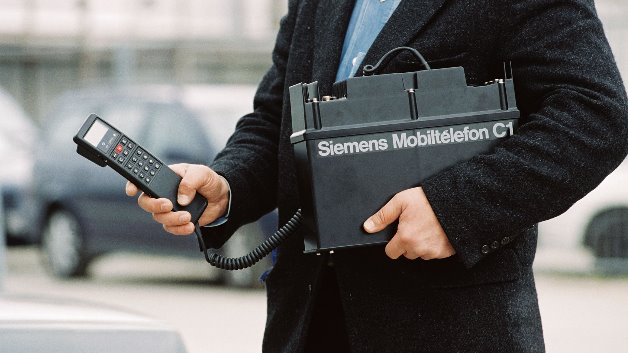
\includegraphics[width=\linewidth]{Kapitel/C-Netz/Grafiken/MobiltelefonC1.jpg}
\captionof{figure}{Mobiltelefon~\cite{c-netz.2}}
\label{fig:c-netz.mobiltelefonEins}
\end{Figure}
Für die damalige Zeit ungewöhnlich waren auch die funktional reich bestückten Hörer, die alle Bedienelemente, LC-Display und LEDs besaßen. 
Das Tastenset war gemäß der CCITT-Empfehlungen aufgebaut und die weitere Mensch-Maschine-Schnittstelle war nach einer FTZ-Richtlinie für alle Hersteller geregelt, so dass der Nutzer keine gerätespezifischen Umstellungsschwierigkeiten hatte, sondern grundsätzlich Zustände wie „eingebucht“, „verbunden“ oder „Sprachverschleierung eingeschaltet“ in bekannter Form angezeigt bekam.

Die Übertragung von Signalisierungsdaten, wurde realisiert durch die Unterteilen des Audiosignals in jeweils 12,5 ms lange Audioblöcke und deren 10 prozentige, zeitliche Kompression, um in die so entstandenen 1,25 ms langen Lücken 4-Bit-Datentelegramme einzufügen.

\subsection*{Vergleich zum A- und B-Netz}
Das C-Netz bot im Vergleich zu den dahin bekannten analogen Mobilnetzen eine Handover-Funktion, die nicht nach der Feldstärke gesteuert wurde, sondern von der relativen Entfernung zur Basisstation. Damit waren Hand-over auch schon unter besten Funkbedingungen möglich, was bei der Netzplanung und der Verdichtung der Frequenzwiederholung ein sehr nützliches Merkmal war. Auch wurde damit die Gleichkanalstörwahrscheinlichkeit deutlich reduziert. Um die relative Entfernungsmessung unterstützen zu können, war jedoch zusätzlicher technischer Aufwand nötig, nämlich eine zeitliche Synchronisation aller Basisstationen zueinander. Für das Realisieren auf Bundesebene bzw. für das Netz, besaß jede Basisstation spezifische Sender und Empfänger für Synchronisationssignale.
Gegenüber dem A-Netz und B-Netz gab es im C-Netz viele „bahnbrechende“ Neuerungen, die heute längst selbstverständlich sind z. B.:
\begin{itemize}
	\item Gemeinsame Vorwahl (0161-) für alle Mobil-Teilnehmer. Man braucht im Gegensatz zum A- und B-Netz nicht mehr zu wissen, wo sich der Teilnehmer aufhält.
	\item Unterbrechungsfreier Wechsel von einer Funkstation zur nächsten (Handover)
	\item Verschleierung des (analogen) Funksignals erschwert unberechtigtes Abhören
	\item Neben fest eingebauten Geräten auch herausnehmbare oder sogar tragbare Geräte möglich
	\item Bis zu 850.000 Teilnehmer (A-Netz 10.500, B-Netz 27.000)
	\item Seit Ende 1990 Anrufbeantworter und Ruf-umleitung als Netzmerkmal (bis dahin nur als Hardware-Zubehör)~\cite{c-netz.3}
\end{itemize}

\subsection*{Einsatz}
Das C-Netz (Funktelefonnetz-C) war ein analoges, zellulares Mobilfunknetz der deutschen DeTeMobil. Es war die dritte und gleichzeitig auch letzte analoge Generation des Mobilfunks, das als System nur in Deutschland, Portugal und Südafrika eingesetzt wurde. Die sehr gute Netzabdeckung von fast 100 Prozent machte das C-Netz zu einer sehr komfortablen Alternative zu den bisherigen Netzen. Das C-Netz wurde primär für telefonische Kommunikationsanwendungen (Autotelefonnetz) mit Zugang zum Telefonnetz und ISDN konzipiert. Das C-Netz wurde vorwiegend für Autotelefone, Küstenschiffe und Eisenbahntelefone benutzt~\cite{c-netz.1}.
Am 31. Dezember 1988 gab es bundesweit bereits 98.762 und im Land Berlin 2.076 C-Netz-Teilnehmer~\cite{c-netz.3}.
\begin{Figure}

\includegraphics[width=\linewidth]{Kapitel/C-Netz/Grafiken/C-Netz_Logo.png}
\captionof{figure}{Logo des C-Netzes~\cite{c-netz.4}}
\label{fig:c-netz.logo}
\end{Figure}
Der Betrieb des C-Netzes wurde am 31. Dezember 2000 eingestellt~\cite{c-netz.6}.

\subsection*{Anbieter und Gremien}
Das C-Netz wurde in Deutschland ausschließlich von der Telekom zur Verfügung gestellt, die dies im Auftrag des Deutschen Staates umsetzte. Zu den Telefonherstellern gehören unter anderem: 
\begin{itemize}
	\item AEG
	\item Bosch
	\item Nokia
	\item Siemens
\end{itemize}
und noch viele andere~\cite{c-netz.5}.

\end{multicols}
\newpage
\section*{Historische Entwicklung}
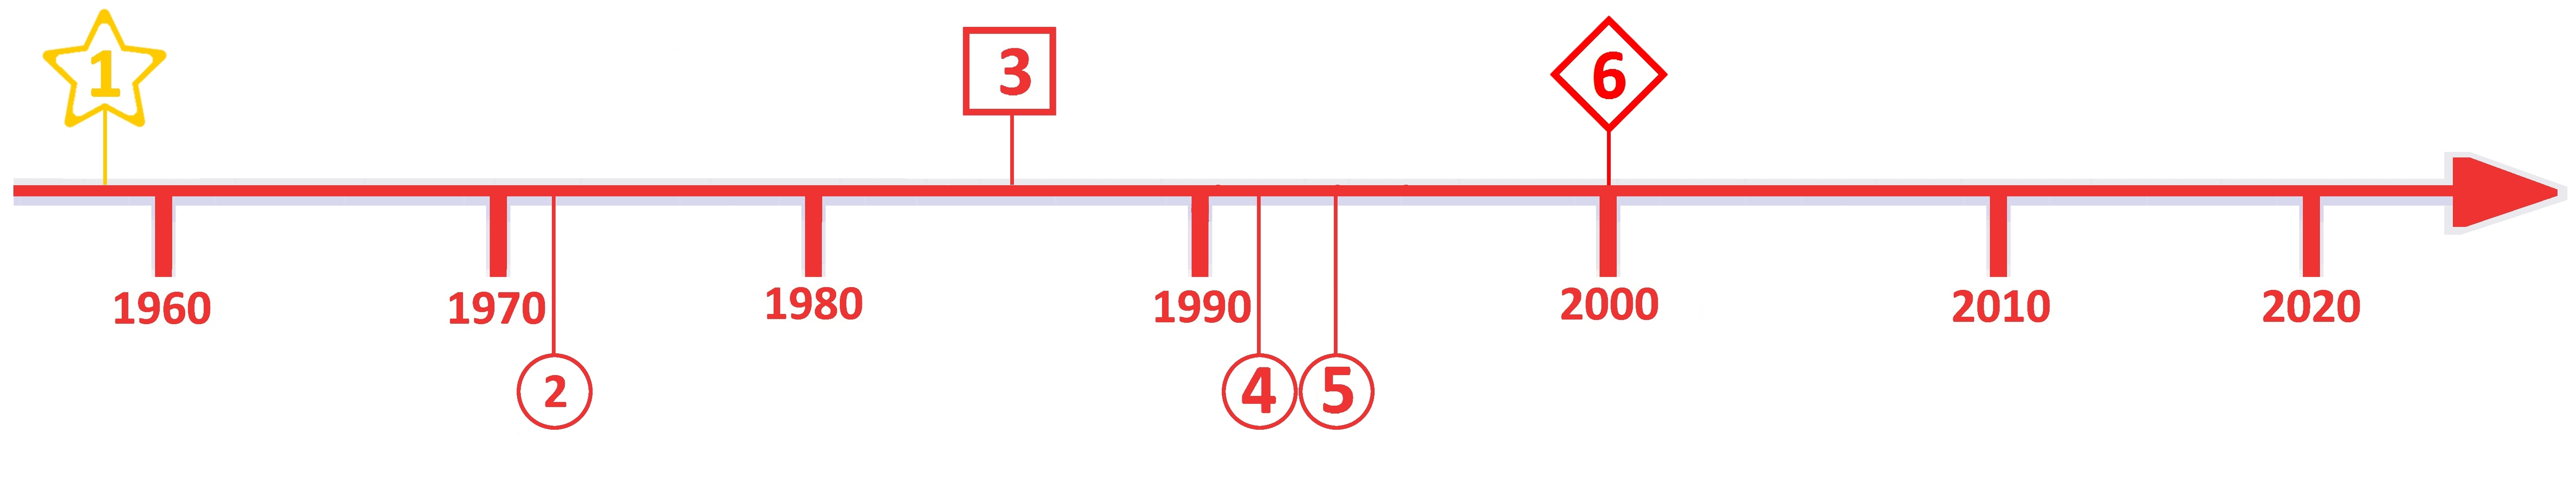
\includegraphics[width=\textwidth]{Kapitel/C-Netz/Grafiken/Zeitstrahl}
\par
\noindent
\begin{tabular}{|p{1 cm}|p{1 cm}|p{15.55 cm}|}
	\hline
	Nummer & Datum & Entwicklungsschritte~\cite{c-netz.7}\\
	\hline
	1 & 1958 & Inbetriebnahme des A-Netzes bis 1977 durch die Bundespost (daraus ging unter anderem die Deutsche Telekom hervor).\\
	\hline
	2 & 1972 & Inbetriebnahme des B-Netzes bis 1994. \\
	\hline
	3 & 1985 & DeTeMobil stellt offiziell das C-Netz zur Verfügung. In Betrieb bis 31.12.2000.\\
	\hline
	4 & 1992 & Deutsche Telekom startet offiziell das D-Netz.\\
	\hline
	5 & 1993 & E-Plus startet das E-Netz.\\
	\hline
\end{tabular}
\par
\begin{multicols}{3}
Das C-Netz wurde im Jahre 1984 (offiziell 1985) in Deutschland eingeführt und ersetzte die umständliche Handhabung des B- bzw. B2-Netzes (Fräulein vom Amt/manueller Verbindungsaufbau). Es war auf Deutschland, Portugal und Südafrika beschränkt, hatte mit einer Netzabdeckung von fast 100 Prozent einen höheren Verbreitungsgrad als das digitale D-Netz bei der Einführung (1991). Dadurch wurde das C-Netz bei Autotelefonen noch bis Mitte der 90er Jahre als erste Wahl eingesetzt, weil es besonders in den ländlichen Gebieten eine bessere Erreichbarkeit hatte als das C-Netz. 
\begin{Figure}
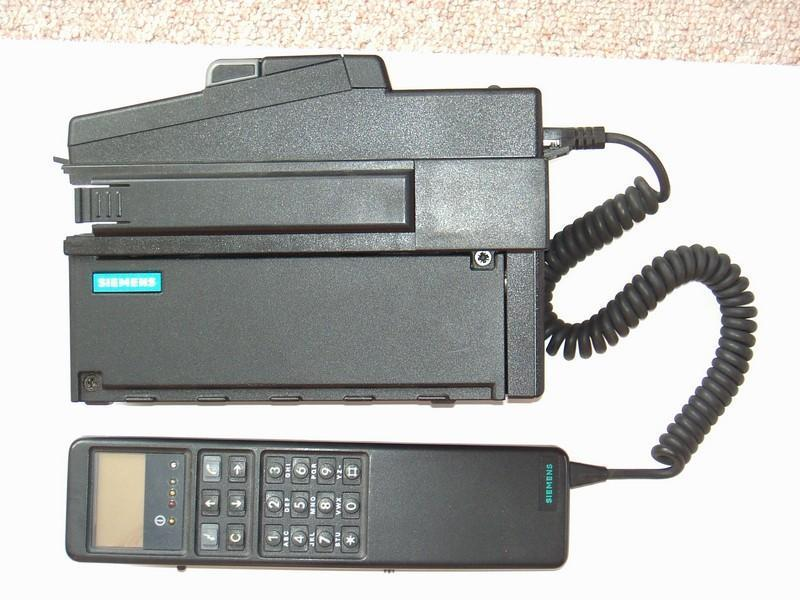
\includegraphics[width=\linewidth]{Kapitel/C-Netz/Grafiken/SiemensC1.jpg}
\captionof{figure}{Mobiltelefon~\cite{c-netz.8}}
\label{fig:c-netz.mobiltelefonZwei}
\end{Figure}
Auch auf Seeschiffen in Küstennähe Deutschlands war ein C-Netz-Gerät an Bord lange weiter verbreitet. Während der Zeit der deutschen Wiedervereinigung 1990 konnten westdeutsche Besitzer von C-Netz-Telefonen bei Aufenthalten in Ostberlin ihr Telefon benutzen und ersparten sich die zeitraubende Zuweisung eines Ferngespräches im DDR-Festnetz~\cite{c-netz.3}.
Der Betrieb des C-Netzes, das am 1. Mai 1985 startete, wurde am 31. Dezember 2000 eingestellt, mit Ausnahme einiger Funkzellen an der deutsch-niederländischen Grenze, die noch einige Monate weiterbetrieben wurden.


\subsection*{Ausblick}
Die Frequenzen des C-Netzes sollen in Zukunft für Railnet (Internet im Zug) genutzt werden. Die Telekom, die das C-Netz bis ins Jahr 2000 betrieb, ist mit ihrer Tochter Telekom Deutschland bei Railnet vertreten. Für die Versorgung im Zug wird WLAN verwendet. Die Verbindung zwischen Zugserver und den stationären Antennen wird mithilfe von Flarion realisiert. Die Datenübertragungsraten von Flash-OFDM liegen maximal bei 3,2 Mbit/s kumuliert, dabei ergeben sich für den Downlink ca. 2,5 Mbit/s und den Uplink ca. 800 kbit/s. Der große Vorteil gegenüber UMTS (Universal Mobile Telecommunications System) sind die geringen Latenzzeiten von unter 50 Millisekunden und eine integrierte Quality-of-Service-Unterstützung. Somit steht jedem Benutzer im Zug eine Breitbandverbindung zur Verfügung. 
Die nordamerikanische Firma Flarion Technologies ist der Entwickler der Flash-OFDM-Technik. Insgesamt sind rund 150 Stationen von Flarion bundesweit auf Sendung. Damit ist eine Abdeckung der Bahnlinien Dortmund–München und Frankfurt am Main–Hamburg gewährleistet (Stand: November 2010)~\cite{c-netz.3}.
Das praktisch unmögliche Roaming in Netze der Nachbarländer war zugleich ein Hauptgrund für die Entwicklung der nächsten Netztechnologie, die erstmals mit dem D Netz ab 1992 zum Einsatz kam~\cite{c-netz.1}. (Bildquelle:~\cite{c-netz.9}) 
\printbibliography[segment=12,heading=subbibliography]
\end{multicols}
\begin{Figure}
\centering
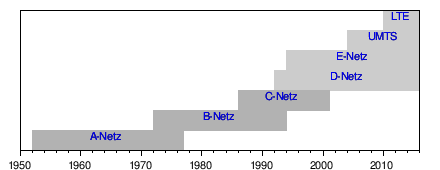
\includegraphics[height=51mm]{Kapitel/C-Netz/Grafiken/ZeitstrahlWiki.png}
\captionof{figure}{Zeitstrahl von A-Netz bis LTE~\cite{c-netz.9}}
\end{Figure}
\newpage
\rowcolors{1}{}{}\begin{multicols}{3}[\section{2G - GSM}]

\rhead{Kevin Taylor, Lucas Lorenz}
\lfoot{16.05.2016}
\newrefsegment

\begin{tabular}{p{2,1 cm}p{2.7 cm}}
\textbf{Steckbrief}& \\
\end{tabular}
\rowcolors{1}{\topicolor!20}{}
\begin{tabular}{p{2,1 cm}p{2.7 cm}}
      Einsatz seit & 1991\\
      Frequenz"-bereich  & 900/1800/\SI{1900}{\mega\hertz}\\
      Datenrate & \SI{9,6}{kbit/s}, \SI{14,6}{kbit/s} (brutto) \\
      Verbreitung & Weltweit\\
      Reichweite & \SI{35}{\kilo\metre} (ideal)\\
\end{tabular}
\par
%ausdünnen?
\subsection*{Überblick}
\textit{2G} (engl. Abk. für second(\textbf{2}nd)-\textbf{g}eneration) ist der Name für die zweite Generation der zellulären Telekommunikationstechnologie, die auf dem \textbf{GSM}-Standard (\textbf{G}lobal \textbf{S}ystem for \textbf{M}obile Communication) basiert. 
GSM wurde mit den folgenden Zielen entwickelt: 
\begin{itemize}
	\item Gute Sprachqualität
	\item Günstig und mobil
	\item Internationale Verfügbarkeit
	\item Effiziente Ausnutzung des Frequenzspektrums
\end{itemize}
Zusätzlich werden GSM-Übertragungen digital verschlüsselt, sodass nur der ausgewählte Empfänger die Nachricht erhalten kann. Außerdem bietet GSM neben der Telefonie auch noch andere Dienste an. Diese sind \textbf{SMS} (\textbf{S}hort-\textbf{M}essage-\textbf{S}ervice), der sich extrem hoher Beliebtheit erfreute, sowie der erste Datendienst mit einer Datenrate von bis zu \SI{14.6}{kbit/s}.
Neben dem 2G-Standard GSM existieren einige weniger verbreitete 2G-Standards wie Nord-Amerikas IS-95 oder Japans PDC.
\cite{G2.1}
\subsection*{Technische Erläuterungen}
%\subsubsection*{Zielsetzung}
\subsubsection*{Grundlegende Technik}
Die Daten werden bei GSM unter Nutzung der Techniken \textit{Frequenzmultiplexing} (\textbf{FDMA} - \textbf{F}requency \textbf{D}ivision \textbf{M}ultiplex \textbf{A}ccess) und \textit{Zeitmultiplexing} (\textbf{TDMA} - \textbf{T}ime \textbf{D}ivision \textbf{M}ultiplex \textbf{A}ccess) übertragen. Die Empfangsrichtung, der Downlink, und Senderichtung, der Uplink, werden durch das FDMA auf verschiedene Frequenzbereiche (Uplink: 890-915Mhz, Downlink: 935-960Mhz) aufgeteilt, welche jeweils aus 124 Kanälen mit jeweils 200kHz bestehen. Die Daten selbst werden mit TDMA versendet und empfangen. Die Rahmenzeit des Zeitmultiplexings beträgt \SI{4,6}{ms} und wird in acht Zeitschlitze aufgeteilt. In einem dieser \SI{0,58}{ms} langen \textit{Bursts} können, unter Einberechnung eines Abzuges für eine Schutzzeit, 148 Bits übertragen werden.
\begin{Figure}
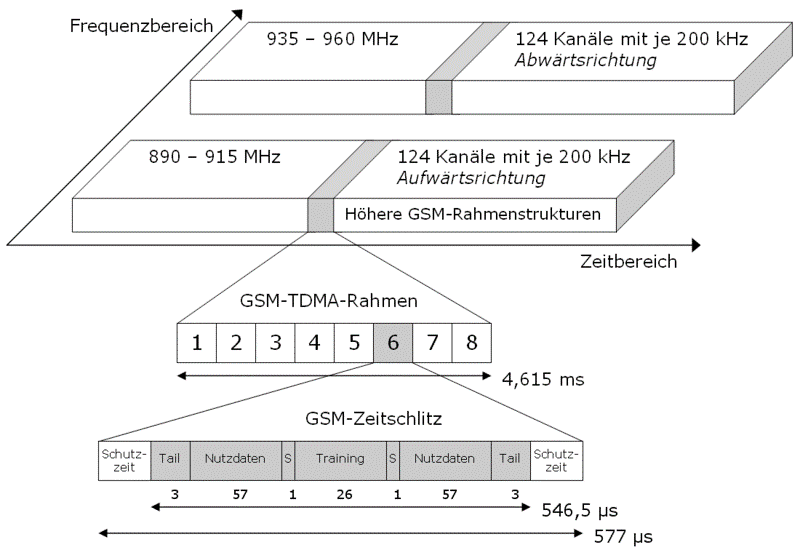
\includegraphics[width=\linewidth]{Kapitel/2G/Grafiken/GSM-Frequenzaufteilung.png}
\captionof{figure}{GSM Frequenzaufteilung~\cite{G2.3}}
\label{fig:G2.frequenzaufteilung}
\end{Figure}
\noindent
Um nun Authentifizierung, Authorisierung und eine korrekte Übertragung zu gewährleisten, werden weitere Bits abgezogen, sodass am Ende eine Datenrate von \SI{9,6}{kbit/s} erreicht wird. \cite{G2.1}\cite{G2.3}
\subsubsection*{Struktur des Mobilfunknetzes}
Aus der vorhergehenden Strukturerklärung ist zu erkennen, dass mit einem solchen System nur rund 1000 Mobilfunkgeräte gleichzeitig genutzt werden können. Dies ist für ein globales Netz aber bei weitem nicht ausreichend. Deswegen kommt nun der zelluläre Aufbau des Netzes zum Tragen, also die Technik des \textit{Raummultiplexing} (\textbf{SDMA} - \textbf{S}pace \textbf{D}ivision \textbf{M}ultiplex \textbf{A}ccess).\cite{G2.2}
\begin{Figure}
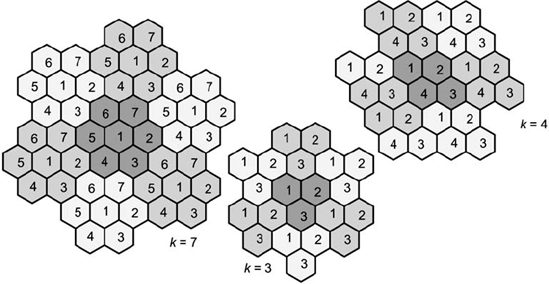
\includegraphics[width=\linewidth]{Kapitel/2G/Grafiken/GSM-Funkzellenideal.png}
\captionof{figure}{GSM Funkzellenideal~\cite{G2.2}}
\label{fig:G2.funkzellenideal}
\end{Figure}
%,height=2.5cm
%letzten beiden Sätze wirken holprig
Um SDMA anzuwenden werden die Frequenzbereiche für Up- und Downlink nochmals unterteilt, um Interferenzen zwischen den unterschiedlichen Netzzellen zu minimieren. Somit haben benachbarte Netzsegmente immer verschiedene Frequenzbereiche. Dies wird mithilfe hexagonaler Waben idealisiert dargestellt (siehe Abb. \ref{fig:G2.funkzellenideal}). In der Realität werden die Strukturen der Netzsegmente, besonders im städtischen Umfeld, durch Häuser, Straßen, Flüsse und andere Faktoren beeinflusst, weshalb von dem wabenförmigen Aufbau abgewichen werden muss (siehe Abb. \ref{fig:G2.funkzellen}).
%Dies ist natürlich eine idealisierte Darstellung, wenn eine bessere Näherung wie in Abb. \ref{fig:G2.funkzellen} aussieht, die insbesondere in städtischem Umfeld durch Häuser, Straßen, Flüsse und anderes beeinflusst wird. \cite{G2.2}
\begin{Figure}
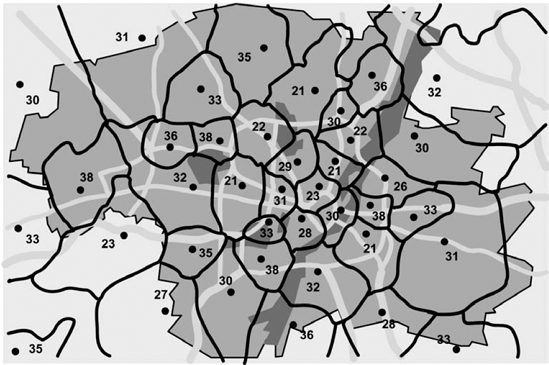
\includegraphics[width=\linewidth]{Kapitel/2G/Grafiken/GSM-Funkzellen.png}
\captionof{figure}{GSM Funkzellen~\cite{G2.2}}
\label{fig:G2.funkzellen}
\end{Figure}
%Einleitung sucked
Es folgt die nächste Überlegung, dass sich mobile Geräte in verschiedenen Zellen aufhalten, oder während eines laufenden Gesprächs von Zelle zu Zelle bewegen. Hierbei erfolgt ein \textit{Hand\-shake} zur Verbindungsübergabe, der den Übergang eines mobilen Gerätes von der aktuellen Funkzelle in die nächste Funkzelle regelt.
Vereinfacht lässt sich dies in Abb. \ref{fig:G2.handshake} beschreiben. Hierbei spricht man von dem Mobilfunkteilnehmer, der sich automatisch in die, in der Bewegungsrichtung befindenden, Basisstation einbucht, während er in der vorherigen Basistation ausgebucht wird.\cite{G2.3}
\begin{Figure}
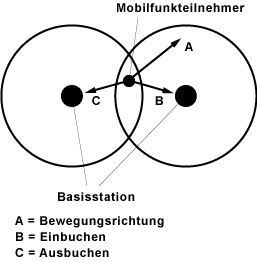
\includegraphics[width=\linewidth]{Kapitel/2G/Grafiken/GSM-Handshake.png}
\captionof{figure}{GSM Handshake~\cite{G2.2}}
\label{fig:G2.handshake}
\end{Figure}
\subsubsection*{SIM}
Das \textit{\textbf{S}ubscriber \textbf{I}dentiy \textbf{M}odule}(siehe Abb. \ref{fig:G2.sim}), kurz \textbf{SIM} oder oft SIM-Card genannt, ist ein Chip, den jedes GSM-Gerät benötigt, um sich in ein, dem GSM-Standard entsprechendes, Funk\-netz einwählen zu können. Diese SIM-Card enthält unter anderem eine \textbf{IMSI} (\textbf{I}nternational \textbf{M}obile \textbf{S}ubscriber \textbf{I}dentity). Diese maximal 15 Zeichen lange dezimale Zahl wird wie folgt aufgeteilt:
\begin{itemize}
	\item Mobile Country Code (MCC), drei Zahlen, International standardisiert (z.B. 262 für Deutschland)
	\item Mobile Network Code (MNC), zwei Zahlen, eindeutige Identifikation eines Netzanbieters des jeweiligen Landes (01, 02, 07 entsprechend für T-Mobile, Vodafone, O2)
	\item Mobile Subscriber Identification Number (MSIN), maximal 10 Zahlen, eindeutige Identifikation eines Nutzers in seinem Heimnetz
\end{itemize}
Darüber hinaus bestitzt die SIM-Card noch die Fähigkeiten PIN, Telefonbuch, Notizbuch, SMS und die zuletzt angerufenen Telefonummern und mehr zu speichern.\cite{G2.1}
\begin{Figure}
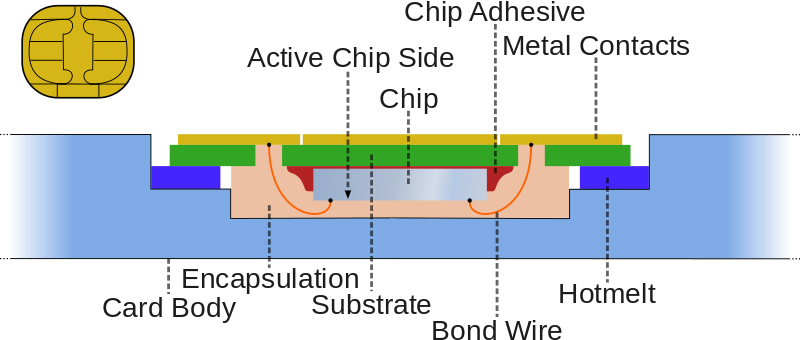
\includegraphics[width=\linewidth]{Kapitel/2G/Grafiken/GSM-SIM.png}
\captionof{figure}{GSM-SIM~\cite{G2.2}}
\label{fig:G2.sim}
\end{Figure}
%eventuell in Tabelle am Anfang reinpacken
\subsubsection*{Sonstiges}
Die Leistungsaufnahme eines solchen mobilen Geräts im 900/1800Mhz Bereich liegt bei 1/2 Watt, während eine passende Basisstation 20-50/10-20 Watt je nach Empfangsdistanz benötigt.\cite{G2.2}
\subsection*{Einsatz}
%klingt doof
Weltweit nutzen 3 Milliarden Menschen GSM als grundlegendes mobiles Kommunikationsmittel. Es ist ungewöhnlich keinen Empfang zu haben, da ein Empfang so gut wie überall möglich ist. (Siehe Abb. \ref{fig:G2.global}).
\end{multicols}
\newpage
\section*{Historische Entwicklung}
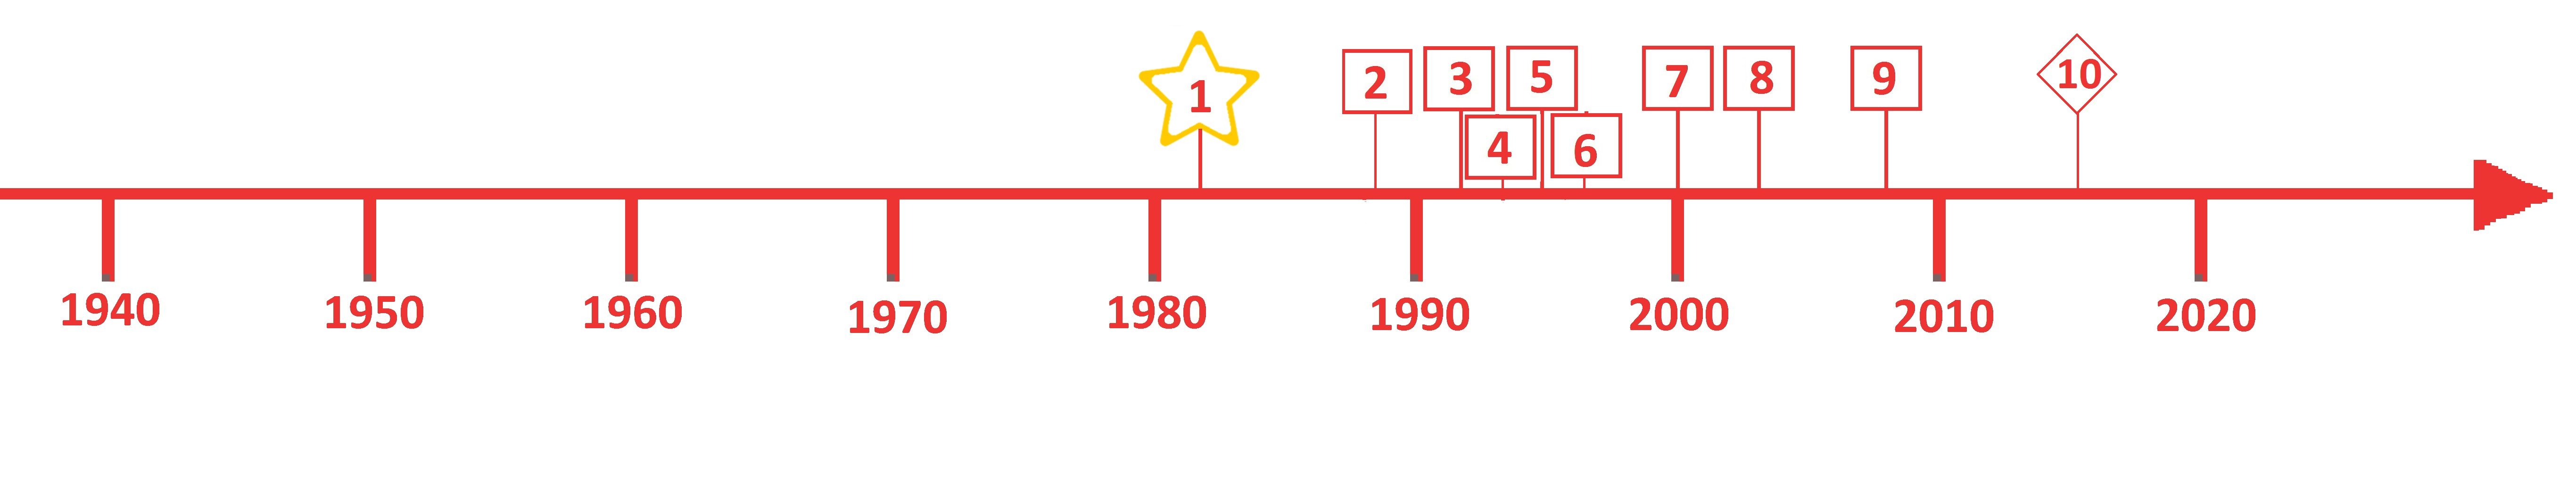
\includegraphics[width=\textwidth]{Kapitel/2G/Grafiken/Zeitstrahl}
\par
\noindent
\rowcolors{1}{\topicolor!20}{}
\begin{tabular}{p{0.5 cm}p{3 cm}p{13.55 cm}}
	Nr. & Datum & Entwicklungsschritte~ \cite{G2.1}\cite{G2.3}\\
	1 & 1982 & Die \textit{Groupe Spécial Mobile} wird eingerichtet und mit der Entwicklung eines globalen Mobilfunkstandards von der CEPT beauftragt.\\
	%CEPT kontrollieren
	2 & 1986 & Die Entscheidung für das 900Mhz Spektrum für das GSM-Band fällt.\\
	3 & 1991 & Der erste GSM-Anruf wurde in Finnland von \textit{Radiolinja} durchgeführt und leutet somit den Beginn des GSM-Mobilfunkstandards ein.\\
	4 & 1992 & Die erste SMS wird versendet.\\
	5 & 1993 & Das erste GSM-Mobiltelefon \textit{Nokia 1011} ist kommerziell erhätlich.\\
	6 & 1995 & Die Dienste über GSM angeboten werden erweitern sich um Fax, Daten und SMS Dienste.\\
	7 & 2000 & \textbf{GPRS} (\textbf{G}eneral \textbf{P}acket \textbf{R}adio \textbf{S}ervice) steht nun zur Verfügung.\\
	8 & 2003 & \textbf{EDGE} (\textbf{E}nhanced \textbf{D}ata Rates for \textbf{G}SM \textbf{E}volution) steht nun zur Verfügung.\\
	9 & 2008 & Weltweit hat der 2G-Mobilfunk mehr als drei Milliarden Nutzer.\\
	10 & 2016 & Erste Mobilfunkanbieter beginnen mit der Abschaltung von GSM-Netzen.\\
\end{tabular}
\par
\begin{multicols}{3}
%ETSI
\subsection*{Organisationen und Standardisierung}
Um ein europaweites Kommunikationsnetz zu entwickeln wurde die \textit{Groupe Spécial Mobile} von der \textbf{CEPT} (\textbf{C}onférence \textbf{E}uropéenne des Administrations des \textbf{P}ostes et des \textbf{T}élécommunications) ins Leben gerufen, die ab 1989 in der \textbf{ETSI} (\textbf{E}uropean \textbf{T}elecommunications \textbf{S}tandards \textbf{I}nstitute) aufging und das heutige Backroynm für GSM (\textbf{G}lobal \textbf{S}ystem for \textbf{M}obile Communication - \textbf{G}roupe \textbf{S}pécial \textbf{M}obile) entstanden ist. Die CEPT bietet für GSM-Operatoren ein Memorandum of Understanding an, was mit einem Standard gleichzusetzen ist, welches 2008 von 747 Mitgliedern unterschrieben wurde, die 670 GSM-Netze in 200 Ländern betreiben. \cite{G2.3}	
%wie schon erwähnt? really? Zielgruppe! 
\subsection*{Ausblick}
Wie schon erwähnt, lag die Nutzerzahl 2008 bei 3 Milliarden Nutzer. Trotzdem fangen erste Länder an G2 auszumustern. Macau ist hierbei Vorreiter, knapp gefolgt von Singapur, Australien und dem größten Mobilfunkanbieter der USA, AT\&T.
Diese Einstellung von GSM würde die Frequenzbereiche für die neueren Standards befreien, doch es gibt auch viele Netzbetreiber, insbesondere in Europa, die sich Zeit lassen, da mit Roaminggebühren, die mit GSM einhergehen, immer noch Geld verdient werden kann.\cite{G2.3}~(Bildquelle:~\cite{G2.4})
\printbibliography[segment=7,heading=subbibliography]
\end{multicols}
\begin{Figure}
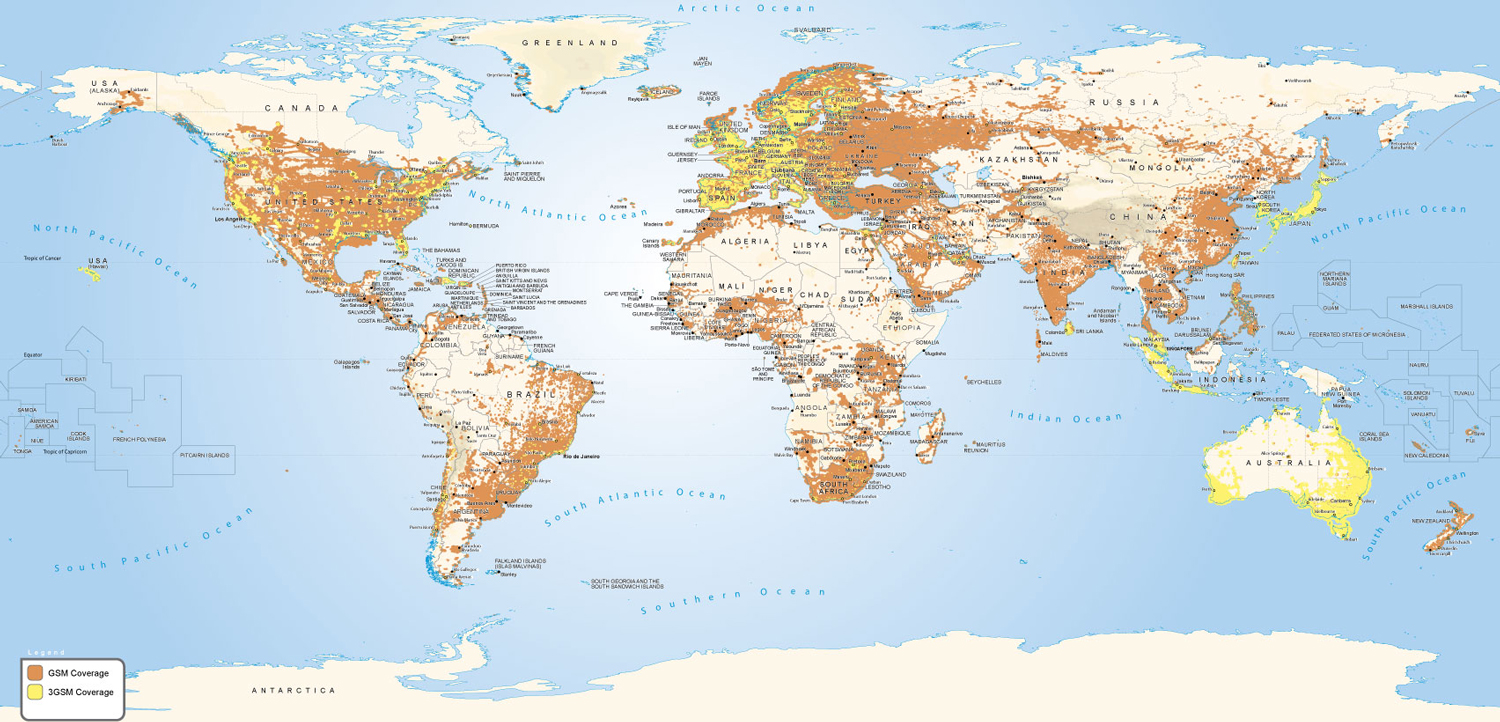
\includegraphics[width=\textwidth]{Kapitel/2G/Grafiken/GSM-Netzabdeckung-Weltweit.jpg}
\captionof{figure}{Globable Netzabdeckung (orange: GSM, gelb: UMTS)~\cite{G2.4}}
\label{fig:G2.global}
\end{Figure}
\newpage

\rowcolors{1}{}{}\begin{multicols}{3}[\section{3G}]

\rhead{Autor: Henrik Scholl}
\lfoot{Letzte Bearbeitung: 17.04.2016}
\newrefsegment

\begin{boxedminipage}{\linewidth}
\begin{tabular}{p{2,1 cm}p{2.7 cm}}
\textbf{Steckbrief}& \\
\end{tabular}
\begin{tabular}{p{2,1 cm}|p{2.7 cm}}
      Einsatz seit & Oktober 2000\\
      \hline
      Frequenz"-bereich  & \SI{5}{\mega\hertz}\\
      \hline
      Datenrate & \SI{13,98}{Mbit/s}\\
      \hline
      Verbreitung & Weltweit\\
      
\end{tabular}
\end{boxedminipage}
\par
%Source http://www.fh-bingen.de/fileadmin/user_upload/Lehrende/Kilsch_Dieter/internet/projekte/TedoSchStiUnits.pdf -> Seite 9 findet ihr alle verwendbaren Einheiten, wie:
%\SI{Zahl}{\mega\hertz} oder \SI{Zahl}{\mili\metre}
%Ich weiß ehrlich gesagt nicht welche Einheiten ihr im Text genau braucht, aber in dem Dokument und mit obigen Beispiel sollte es umsetzbar ein.
\subsection*{Überblick}
3G oder auch UMTS (Universal Mobile Telecommunications System) wird als dritte Generation des Mobilfunkstandarts bezeichnet, es ist somit die Weiterentwicklung des GPRS-Dienstes. Schon im Jahr 2000 konnte Deutschland die Lizenzen an dieser Technologie erwerben, für den damaligen Preis von 98,8 Milliarden DM. Innerhalb Deutschland wurden diese Lizenzen an sechs Mobilfunkbetreiber weiterverkauft für einen Preis von je 16 Milliarden DM. Dazu mehr in dem Abschnitt Anbieter und Gremien. Der große Durchbruch war der Technologie bei der Einführung in den Markt nicht vergönnt. Durch hohe Kosten für den Endnutzer wurde nur zögerlich zu 3G gegriffen. Auch für die Firmen war der Einstig in dieses Segment nicht einfach. Durch die hohen Kosten der Lizenz schwand die Liquidität der Firmen und dies hatte einen Wertverlust an der Börse zur Folge. Auch die Ausbleibenden Nutzer waren anfangs ein Problem. Insgesamt verhinderten die hohen Lizenzgebühren einen zügigen Netzausbau. Erst 2003 konnten ersten Probeläufen mit einigen Firmenkunden unternommen werden und ab 2004 wurde es in Deutschland kommerziell genutzt.  
Die Weiterentwicklung von UMTS mittels eines nennt man HSDPA (High Speed Downlink Packet Access). Da HSDPA einen Fortschritt gegenüber UMTS darstellt, aber auf derselben Basis arbeitet, wird es nicht als 4G Netz sondern 3.5G oder auch 3G+ bezeichnet. Den deutschen Markt erreichte HSDPA erst Anfang 2006 und wurde gegen Ende dieses Jahres für einige Geschäftskunden zur Verfügung gestellt. ~\cite{3G.1, 3G.2}


\subsection*{Technische Erläuterungen}
\subsubsection*{UMTS}
Technisch gesehen ist UMTS eine Weiterentwicklung des GSM/GPRS- Architektur, welche anfänglich nur durch eine veränderte Software, bei gleich bleibenden Kernnetz, entstand. Das Zugangsnetz hingegen ist eine Neuentwicklung mit dem Namen UMTS Terrestrial Radio Access Network (UTRAN). Wie der Abbildung 1 entnommen werden kann besteht die UMTS-Referenzarchitektur aus insgesamt drei Bereichen, oder auch Domains. 
Die User Equipment Domain (UED) ist nochmals in zwei Bereich unterteil, die Universal Subscriber Identity Module Domain (USIM Domain) und die Mobile Equipment Domian (MED), was die Engeräte beschreibt, welche eine SIM-Karte besitzen. Die UED ist für die Authentisierung zuständig und über eine Luftschnittstelle Uu mit der Access Network Domain (AND) verbunden. 

\begin{Figure}
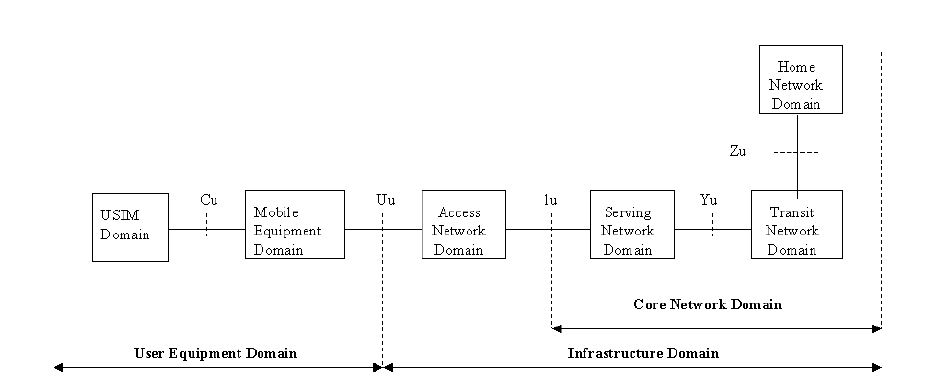
\includegraphics[width=\linewidth]{Kapitel/3G/Grafiken/Domains.jpg}
\captionof{figure}{Übersicht Domains~\cite{3G.1}}
\label{fig:vorlage.vorlesungssaal}
\end{Figure}
 
Die AND wird bei UMTS durch UMTS Terrestrial Radio Access Network (UTRAN) umgesetzt und ermöglicht die Ankopplung eines Mobiltelefons an das Core Network. Der Aufbau von UTRAN besteht aus mehreren Radio Network Subsystems (RNS). Diese werden jeweils von einem Radio Network Controller (RNC) gesteuert. Hierbei hat der RNC mehrere Aufgaben, wie beispielsweise die Ver – und Entschlüsslung, die Staukontrolle sowie weitere Verwaltungsaufgaben. Ein solcher RNC verwaltetet hierbei einen oder mehrere Node B (Basisstationen), wobei eine solche Node B eine oder mehrere Antennen Steuert. Die Antennenanzahl bedingt dann wiederum das Aufspannen einer oder mehrer Funkzellen.

Die Core Network Domain (CND) ist auch als Kernnetz bekannt und ermöglicht Verbindungen in das eigene Netz oder in andere Systeme. Hierbei wird CND nochmals in Serving Network Domain (SND), Home Network Domain (HND) und Transit Network Domain (TND) aufgeteilt. In diesen Bereichen wird das Routing, die Lokalisierung, das Roaming, das Billing und das Charging umgesetzt. Weiterhin wird das Kernnetz in zwei weitere Bereiche eingeteilt. Einmal in die Circuit Swiched Domain, welche der Leitungsvermittlung dient und andererseits in die Packet Switched Domain, diese dient zur Paketvermittlung. Diese Unterscheidung ist bedingt durch die Dienste, welche mittelst des Dienstes genutzt werden. So sind Datendienste, wie das Verschicken eines Bildes auf die Paketvermittlung, angewiesen und Telefongespräche auf eine Leitungsvermittlung.  Diese Abtrennungen der beiden Domains sind oftmals nur Modellhaft, die tatsächliche Umsetzung besteht lediglich nur aus einem Bauteil. Eine weitere Aufgabe des Kernnetzes ist die Verwaltung von mehreren Mobile-service Switching Centre (MSC) beziehungsweise Serving GPRS Support Nodes (SGSN) in den einzelnen RNS. Hierbei verwaltet nun jede MSC zusätzlich eine Home Location Register (HLR), welches die Nutzerdaten beheimatet und ein Visitor Location Register (VLR). Der Abbildung 2 kann ein solcher modellhafter Aufbau entnommen werden.

\begin{Figure}
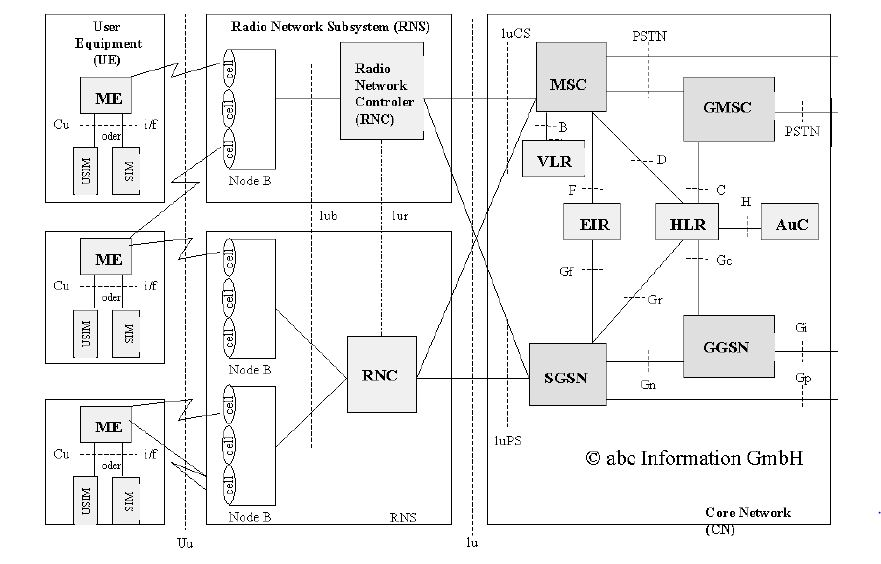
\includegraphics[width=\linewidth]{Kapitel/3G/Grafiken/Architektur.jpg}
\captionof{figure}{Architektur UMTS ~\cite{3G.1}}
\label{fig:vorlage.vorlesungssaal}
\end{Figure}

Die Direct-Sequence-(DS)-CDMA-Technik macht nun großen Unterschied zwischen GSM und UMTS im Bereich der Funkschnittstelle aus. Hierbei steht CDMA für ein Codemultiplexverfahren, welches einen Datenstrom mit einer Chipping-Sequenz multipliziert. Der so erzeugt Code wird im Anschluss daran abhängig von dem Netzbetreiber über einem Frequenzband gespreizt, üblich sind hierbei Bandbreiten zwischen 4,4 MHz und 5 MHz. Durch die auf Spreizung können Störungen verringert werden und weiterhin bei einer bestimmten Spreizung eine Trennung des Signals von Hintergrundgeräuschen, ohne Kenntnisse des Codes, ausgeschlossen werden.~\cite{3G.1, 3G.4}


\subsubsection*{HSDPA}
HSDPA wurde als Weiterentwicklung von UMTS mit dem 5. Release eingeführt.  Der große Vorteil von HSDPA besteht darin das es neben UMTS koexistieren kann und auch auf der Technologie von UMTS aufbaut. Eine Erneuerung war die verkürzte Latenzzeit von 100 ms. Weiterhin kann HSDPA nun die Leistung einer Funkzelle dauerhaft nutzen, was durch einen neuen Funkkanal erreicht wurde. Die Steuerung des Nutzkanals übernimmt hierbei der High Speed Dedicated Physical Control Channel (HS-SCCH). Durch High Speed Downlink Shared Channel (HS-DSCH) und High Speed Physical Shared Channel (HS-PSCH) konnte die verbesserte Übertragungsgeschwindigkeit erreicht werden. Auch das Short Transmission Time Interval (STTI), die Zeit die die Übertragung eines Datenpakets benötigt, wurde um ein Fünftel verringert und beträgt somit 2 ms.  Auch das Multiplexing würde bei HSDPA durch die Kombination von CDMA und TDMA (Zeitmultiplexing) verbessert. Durch die Einteilung der Zeitachse in mehre Bereiche können jedem Nutzer ein Zeitbereich bereitgestellt werden. Dieser Bereich hat dann die STTI-Zeitdauer.~\cite{3G.1, 3G.3}

\subsection*{Einsatz}

Nachdem nun der theoretische Aufbau bekannt ist, folgt eine Erläuterung zum Aufbau einer Sprach- oder Datenverbindung. Zu Beginn muss jedes Mobiletelefon eine SIM-Karte besitzen und sich in einem HLR registrieren. Im nächsten Schritt muss eine Verbindung zu einer Basisstation aufgebaut werden. Dieser Wunsch nach dem Aufbau einer Verbindung leitet die Basisstation weiter zu dem RNC, der diese ebenfalls an den MSC weiter gibt. Dort angekommen ordnet der MSC die Telefonnummer dem Nutzer zu und durch Routing kann nun das HLR angesprochen werden. Im Anschluss daran wird die Position bzw. die Zelle in der sich das Mobilfunkgerät eingewählt hat dem HLR übermittelt. Der Ort wird im HLR vermerkt und es werden ein Teil der Nutzerdaten an das VLR der aufrufenden MSC gesendet. Nun wird das Mobiltelefon authentifiziert und daraufhin kann ein Telefongespräch mit diesem Gerät geführt werden. Dazu muss nun erneute der Wunsch durch die Basisstation an die RNC und im Anschluss da-

\end{multicols}
\newpage
\section*{Historische Entwicklung}
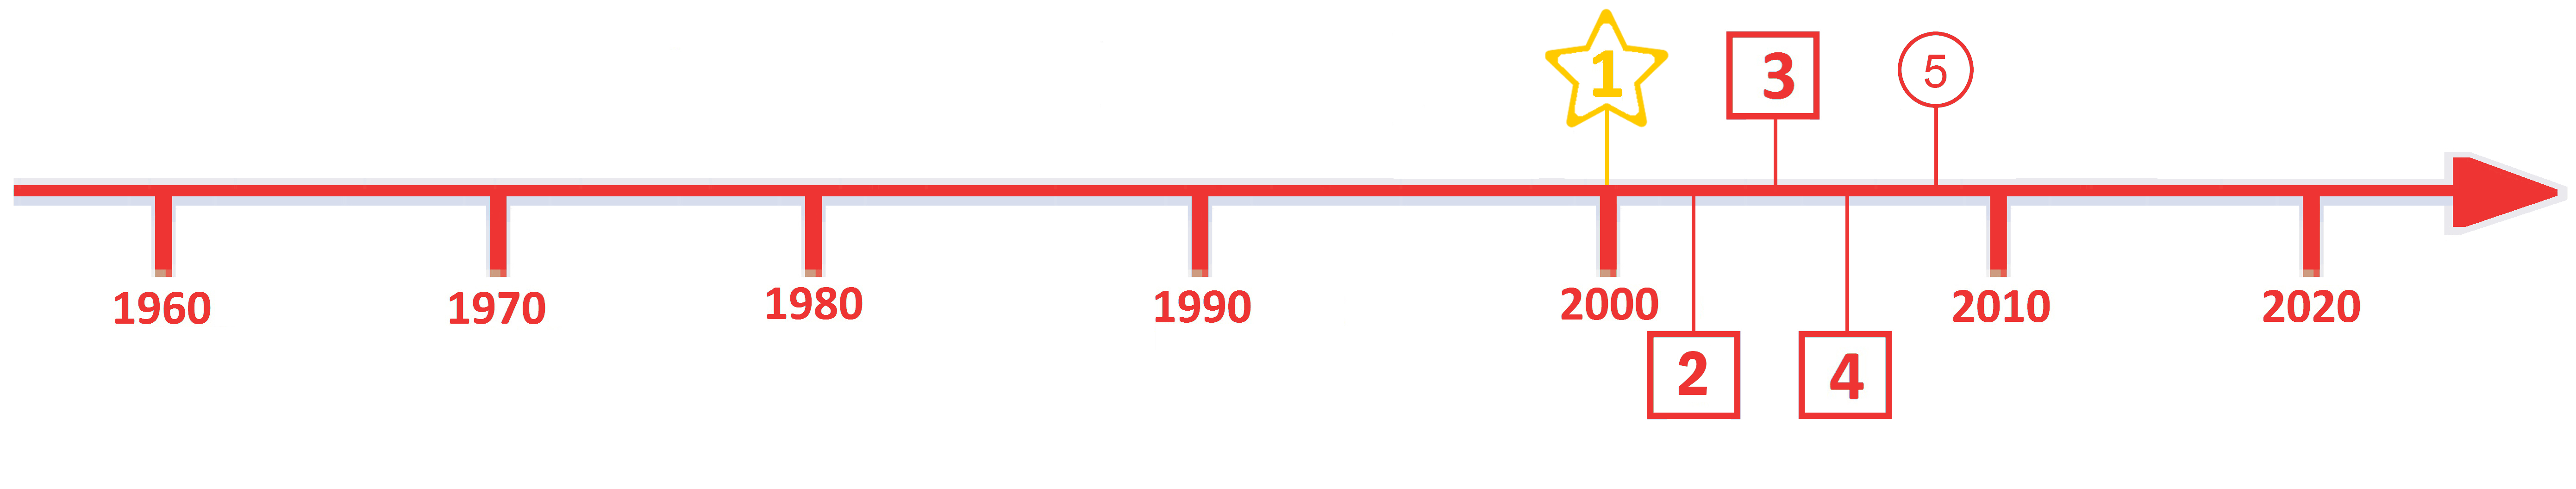
\includegraphics[width=\textwidth]{Kapitel/3G/Grafiken/Zeitstrahl}
\par
\noindent
\begin{tabular}{|p{1 cm}|p{3 cm}|p{13.55 cm}|}
	\hline
	Nummer & Datum & Entwicklungsschritte ~\cite{3G.2}\\
	\hline
	1 & 2000 & Einführung von UMTS in den deutschen Markt\\
	\hline
	2 & 2004 & Einführung von UMTS fähigen Endgeräten\\
	\hline
	3 & 2006 & Einführung von HSDPA in den deutschen Markt\\
	\hline
	4 & ab 2007 & Hohe Netzabdeckung von UMTS und HSDPA innerhalb von Deutschland \\
	\hline
\end{tabular}
\par
\begin{multicols}{3}


ran an die MSC weitergeleitet werden. Soll nun ein anderes Mobiltelefon angerufen werden, wird dieses durch die HLR aufgerufen, denn dort sind Positionsdaten gespeichert. Daraufhin kann die Zelle angesprochen werden in dem sich das Mobiltelefon befindet und der Anruf kann getätigt werden. 
Durch den Dezentralen Aufbau dieses Netzes kann ein Gesamtausfall vermieden werden da höchstens Teilgebiete des Mobilfunkproviders ausfallen können. ~\cite{3G.1}

\subsection*{Anbieter und Gremien}
Wie bereits erwähnt lag der Ausbau dieser Netze an den Firmen, welche als erstes Lizenzen für UMTS ergattern konnten. Die Firmen T-Mobile Deutschland GmbH, Vodafone D2 GmbH, MobilCom Multimedia GmbH, Auditorium Investments Germany S.à.r.l. (später umformiert in E-plus 3G Luxemburg S.à.r.l.), O2 und Group 3G (ein Konsortium aus der spanischen Telefónica und der finnischen Sonera)erhielten diese zu Beginn.  Doch in den Folgejahren geben die Firmen MobilCom Multimedia GmbH und Group 3G ihre Lizenzen wieder ab.
Die HSDPA Netzanbieter von Deutschland sind T-Mobile, Vodafone, o2 und E-Plus. Alle bekannten Anbieter von 3G Tarifen nutzen das Netz einer dieser Provider. 
~\cite{3G.1, 3G.2}

\subsection*{Ausblick}
Der nächste Schritt in der Evolutionären Entwicklung des mobilen Internets ist 4G oder auch LTE (Long Term Evolution). Mitte August des Jahres 2010 wurde in Deutschland der erste LTE-Sendemast errichtet. Aber nahere Erläuterungen zu LTE finden Sie im folgenden Artikel ~\cite{3G.2}.


\printbibliography[segment=13,heading=subbibliography]
\end{multicols}



\newpage
\rowcolors{1}{}{}\begin{multicols}{3}[\section{4G/LTE}]

\rhead{Autorin: Yuliya Ukolava}
\lfoot{Letzte Bearbeitung: 17.04.2016}

\newrefsegment

\begin{boxedminipage}{\linewidth}
\begin{tabular}{p{2,1 cm}p{2.7 cm}}
\textbf{Steckbrief}& \\
\end{tabular}
\begin{tabular}{p{2,1 cm}|p{2.7 cm}}
      Einsatz seit & 2009\\
      \hline
      Frequenz"-bereich  & \SI{ 20 }{\mega\hertz}\\
      \hline
      Datenrate & \SI{100}{bit/s}\\
      \hline
      Verbreitung & Weltweit\\
\end{tabular}
\end{boxedminipage}
\par

\subsection*{Überblick}
LTE steht für Long Term Evolution (langfristige Entwicklung) und folgt als vierte Mobilfunkgeneration (4G) auf die vorigen Standards GSM (2G) und UMTS (3G). ~\cite{4GLTE.1}
Es soll besonders schnelle Geschwindigkeiten beim Surfen im mobilen Internet ermöglichen. 


\subsection*{Technische Erläuterungen}
Um den wachsenden Datenverkehr im Mobilfunknetz abwickeln zu können ist eine breitbandige Anbindung der Basisstationen an das Kernnetz erforderlich. Hierfür setzt man bevorzugt Richtfunk und Glasfaser ein. Das Transportnetz, das die Basisstationen mit dem Kernnetz verbindet besteht hauptsächlich aus Routern und Switche, wie sie üblicherweise in der Netzwerktechnik eingesetzt werden. Damit das möglich ist, sind in LTE gängige Netzwerktechniken und -protokolle zusammengeführt. Die Systemarchitektur von GSM und UMTS bestand hauptsächlich noch aus teurer Spezialhardware.

Um die Übertragungskapazität zu erhöhen wird beim Informationsaustausch zwischen Basisstation und dem Kernnetz gespart. Angestrebt wird eine einfache Integration in das bestehende Mobilfunknetz und eine einfache Architektur mit sich selbst konfigurierenden Basisstationen.
Die LTE-Basisstationen sind kleiner als GSM- und UMTS-Basisstationen. So können die Netzbetreiber die LTE-Basisstationen an Orten installieren, die sich für GSM- und UMTS-Basisstationen weniger eignen. Das erlaubt die Funkversorgung von Orten, die sonst nur schwer oder gar nicht zugänglich sind.

Die LTE-Netzarchitektur wird als Evolved Packet System (EPS) bezeichnet. Es wird in das Funkzugangsnetz Evolved UMTS Terrestrial Radio Access Network (EUTRAN) und das Kernnetz Evolved Packet Core (EPC) unterteilt. Das EPC ist vollständig paketorientiert und setzt auf das Internet Protokoll (IP).
\begin{Figure}
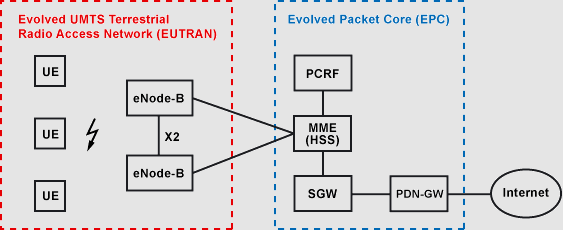
\includegraphics[width=\linewidth]{Kapitel/4GLTE/Grafiken/Modell.png}
\captionof{figure}{EPS - Evolved Packet System~\cite{4GLTE.2}}
\label{fig:vorlage.vorlesungssaal}
\end{Figure}

Im EUTRAN werden die mobilen Endgeräte als User Equipment, kurz LTE UE, bezeichnet. Die Funktion der Basisstationen ist aus der UMTS-Netzarchitektur abgeleitet und tragen deshalb die Bezeichnung eNode-B. In der LTE-Netzarchitektur sind die Basisstationen mit ihren benachbarten Basisstationen und dem Kernnetz verbunden. Die Schnittstelle X2 zwischen den Basisstationen ermöglicht schnelles Handover.
Für die Anmeldung der Teilnehmer am Netz und deren Lokalisierung ist die Management Mobility Entity (MME) zuständig. Die MME greift auf den Home Subscriber Service (HSS) zu. Hat das Endgerät einen gültigen Account wird ihm ein Serving-Gateway (SGW) zugewiesen. Von dort besteht eine Verbindung zum PDN-GW, dass die Verbindung zum Internet herstellt und dem Endgerät eine IP-Adresse zuweist.
Im Kernnetz befindet sich außerdem die PCRF (Policy and Charging Rules Function). Hier werden die Leistungen, die im Tarif festgelegt sind, geregelt. ~\cite{4GLTE.3}

Damit mehrere Mobilfunkgeräte gleichzeitig Daten übertragen können arbeitet LTE mit skalierbaren und individuellen Kanälen. Das bedeutet konkret, dass das Frequenzspektrum geteilt und einzelnen Geräten für eine bestimmte Zeit zugewiesen wird.
Für den Downlink wird OFDMA verwendet. OFDMA teilt das zur Verfügung stehende Frequenzband in viele schmale Bänder (Kanäle) auf. Das bedeutet, dass LTE mit unterschiedlich großen Frequenzbändern auskommen. Die Bandbreite wird flexibel genutzt, um das Äußerste an Übertragungsleistung aus den Frequenzen herauszuholen.

Das Frequenzband (\si{10},\si{15},\SI{20}{\mega\hertz}) wird in Subcarrier zu je \SI{15}{\kilo\hertz} aufgeteilt. Jeweils 12 Subcarrier werden zu einem Ressource-Block (RB) zusammengefasst, was die kleinste Einheit dessen ist, was einem LTE-Gerät zugewiesen werden kann. Ein Gerät kann je Richtung einen bis mehrere Ressource-Blöcke belegen. Die Anzahl hängt von der Auslastung der Zelle und der Signalgüte ab. Die Obergrenze ergibt sich aus der Breite des Frequenzblocks, den die Basisstation verwendet. Bei einem \SI{10}{\mega\hertz}-Frequenzblock sind das 50 Ressource-Blöcke. Bei \SI{20}{\mega\hertz} sind es 100.

Zeitlich ist die Übertragung eines Blocks auf \SI{10}{\milli\second} festgelegt (Frame). Das sind 10 Blöcke pro Sekunde. Jeder Frame besteht wiederum aus 10 Subframes. Pro Subframe lässt sich ein Transport-Block übertragen. Die Größe des Transport-Blocks hängt im wesentlichen von der Signalgüte ab. Die Signalgüte bestimmt, welche Modulation verwendet wird, wie das Verhältnis zwischen Nutzdaten und Fehlerkorrektur (Code-Rate) ist und wie viele Ressource-Blöcke verwendet werden. Dabei hängen diese drei Parameter direkt miteinander zusammen.

Spezielle Algorithmen wählen die geeigneten Kanäle aus und berücksichtigen dabei die Einflüsse aus der Umgebung. Dabei werden nur die Träger zur Übertragung genutzt, die für den Nutzer am günstigsten sind.
Für den Uplink wird SC-FDMA verwendet (Single Carrier Frequency Division Multiple Access). Das ist ein Einträgerzugriffsverfahren und OFDMA sehr ähnlich. SC-FDMA weist geringer Leistungsschwankungen auf und macht einfacher Leistungsverstärker möglich. Das schont vor allem den Akku mobiler Geräte.

LTE arbeitet auch mit räumlich separierte Datenströmen. Die LTE-Spezifikation sieht 4 Antennen in der Basisstation und 2 Antennen in den Endgeräten vor. Das Sendesignal wird zur Übertragung an mehrere Sendeantennen weitergeleitet. Die Empfangssignale werden von zwei Antennen empfangen (MIMO). Aus beiden Signalen wird dann ein besseres Signal herausgerechnet. Damit erreicht man einen besseren Datendurchsatz, weil beide Sende- und Empfangspfade nicht den gleichen Störungen (Verluste und Interferenzen) unterliegen. Dieses Verfahren ist in abgewandelter Form auch in WLANs nach IEEE 802.11n spezifiziert. Zusätzlich verwendet LTE, wie HSPA auch, das gleiche Shared-Channel-Prinzip, sowie HARQ und AMC. ~\cite{4GLTE.4}
 

\subsection*{Einsatz}
„Anytime-anywhere“, also immer und überall mobile Kommunikation betreiben zu können, dafür soll 4G stehen. Primär soll das heißen: ortsunabhängiger drahtloser Breitband-Internetzugang. Multimedia Messaging Service (MMS), Video Chat, High Definition Radio (HD-Radio), mobile TV, High Definition TV content (HDTV), DVB und normales Telefonieren soll in diesem Netz möglich sein.
LTE bietet als rein paketbasiertes Netz keinen separaten, verzögerungsfreien Kanal für Sprachdaten an. Daher können Telefonate im LTE-Netz ausschließlich per Voice over IP übertragen werden. Zum Telefonieren muss sich ein Handy derzeit beim LTE-Netz abmelden und ins 3G- (UMTS) oder 2G-Netz (GSM) wechseln. Bei diesem Circuit Switch Fallback (CSFB) genannten Verfahren entstehen beim Rufaufbau Verzögerungen von einigen Sekunden. ~\cite{4GLTE.5}
Durch die bessere Ausnutzung der Frequenzen ist es möglich, mehr Benutzer gleichzeitig mit Daten zu versorgen, woraus sich ein geringerer Preis pro Datenpaket ergibt. 
Am meisten aber dürften die Bewohner ländlicher Gegenden von der neuen 4G-Technik profitieren: War dort bis jetzt nur sehr langsames oder gar kein DSL möglich, so kann man nun die entsprechenden Orte per Mobilfunk anbinden und so mit schnellen Internet-Zugängen versorgen. ~\cite{4GLTE.6}

\end{multicols}
\newpage
\section*{Historische Entwicklung}
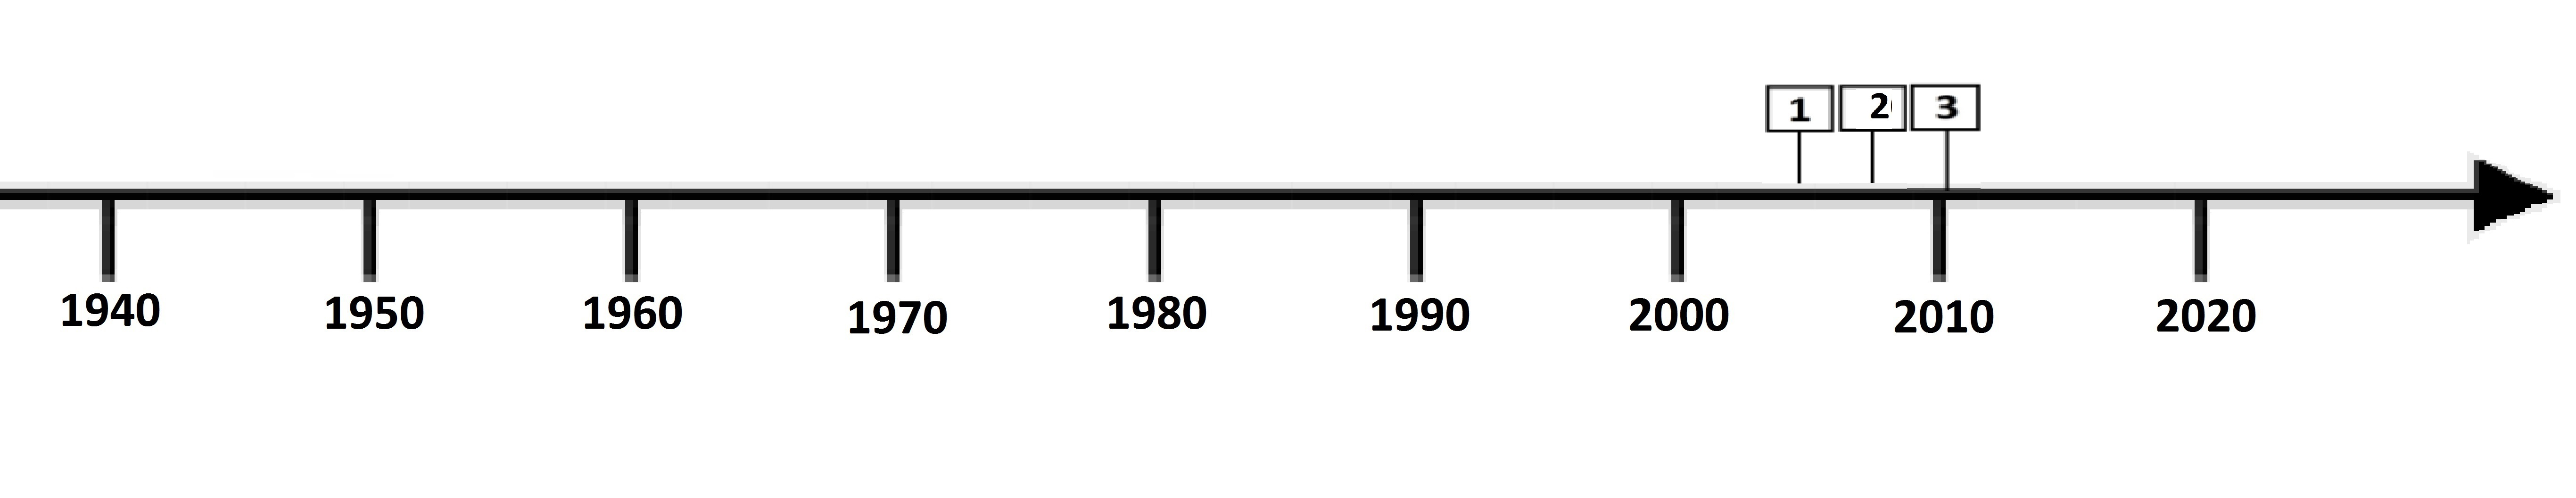
\includegraphics[width=\textwidth]{Kapitel/4GLTE/Grafiken/Zeitstrahl}
\par
\noindent
\begin{tabular}{|p{1 cm}|p{3 cm}|p{13.55 cm}|}
	\hline
	Nummer & Datum & Entwicklungsschritte\\
	\hline
	1 &  September 2006 & Siemens Networks, heute Nokia Solutions and Networks, zusammen mit der Nomor Research GmbH zeigt erstmals einen Emulator eines LTE-Netzwerks mit Live-Applikationen.\\
	\hline
	1 & November 2006 & Die erste LTE-Demonstration in Hongkong in der Öffentlichkeit. \\
	\hline
	2 & 2008 & Auf dem GSMA Mobile World Congress in Barcelona zeigte Ericsson erstmals eine Ende-zu-Ende-Verbindung mit LTE auf kompakten Mobilgeräten. Es wurden Datenraten von \SI{25}{Mbit/s} im Uplink und Downlink demonstriert.\\
	\hline
	2 & Im März 2008 & In einem Feldtest von NTT DoCoMo werden \SI{250}{Mbps} demonstriert.\\
	\hline
	2 &  Ende 2008 &  Es wird von LG ein LTE-Chip vorgeführt, welcher Datenraten von \SI{60}{Mbps} erreicht, was etwa dem Achtfachen der HSDPA-Cat8-Datenrate von \SI{7,2}{Mbps} entspricht.\\
	\hline
	3 & 14. Dezember 2009 & Die ersten kommerziellen LTE-Netzwerke von TeliaSonera werden in Stockholm und Oslo in Betrieb genommen.\\
	\hline
	3 & Mai 2010 & In Deutschland wird LTE mit der Frequenzversteigerung durch die Bundesnetzagentur im  eingeführt.\\
	\hline
\end{tabular}
\par
\begin{multicols}{3}
\subsection*{Anbieter und Gremien} 

Die Deutsche Telekom/T-Mobile, Vodafone, o2 und E-Plus sind die deutschen LTE-Anbieter. Der Düsseldorfer Netzbetreiber E-Plus ist erst im März 2014 mit 4G gestartet. Die beste LTE-Netzabdeckung in Deutschland in der Fläche bieten aktuell die Deutsche Telekom und Vodafone. Diese beiden Anbieter sind auf dem Land (LTE als DSL-Ersatz) und in den Städten stark mit 4G vertreten, während o2 und E-Plus in den Städten eine echte Alternative zu den großen Netzbetreibern sind.
Der 4G-Ausbau der LTE-Anbieter geht in Deutschland seit dem LTE-Start schnell voran. Seit November 2012 haben die deutschen Netzbetreiber ihre Versorgungsverpflichtungen erfüllt und alle Weißen Flecken in den einzelnen Bundesländern geschlossen. Heute beträgt die LTE-Abdeckung deutschlandweit mittlerweile 69 Prozent. Viele deutsche Großstädte bieten dazu eine ausgezeichnete 4G-Netzabdeckung von über 90 Prozent. Nutzer können dort bei einem Anbieter wie T-Mobile oder Vodafone in gut ausgebauten Netzen mit bis zu \SI{150}{Mbit/s} surfen. ~\cite{4GLTE.7}

\subsection*{Ausblick}
Generell zeigt die Prognose, dass der Bedarf an schnellem Internet für unterwegs stetig wächst und auch die Ansprüche der Nutzer an die Mobilfunkanbieter wachsen. Diese Entwicklung geht einher mit immer schneller und besser werdenden Smartphones und Tablets, die unter anderem dafür genutzt werden, Medieninhalte via Streaming mobil auf das jeweilige Gerät zu bringen. Hierbei ist eine leistungsstarke, mobile Datenverbindung natürlich unabdingbar. 4G gibt viele Möglichkeit im Bereich mobiler Datenübertragung und durch steigende 4G-Netzabdeckung und Einführung von LTE als „echten“ DSL-Ersatz soll dieser Bedarf abgedeckt werden. Aber es gibt immer noch viel Potenzial und Erweiterungsoptionen. Deswegen wird es inzwischen bereits am 4G-Nachfolger 5G gearbeitet. 


\printbibliography[segment=9,heading=subbibliography]
\end{multicols}


\newpage

\rowcolors{1}{}{}\begin{multicols}{3}[\section{5G}]

\rhead{Lucas Lorenz, Jan Selig}
\lfoot{15.05.2016}

\newrefsegment

\begin{tabular}{p{2,1 cm}p{2.7 cm}}
\textbf{Steckbrief}& \\
\end{tabular}
\begin{tabular}{p{2,1 cm}p{2.7 cm}}
\rowcolors{1}{\topicolor!20}{}
      Einsatz ab & voraussichtlich 2020\\
      Frequenz"-bereich  & mm-Band (\SI{24.25}{\giga\hertz}-\SI{86}{\giga\hertz}) 		  oder  C-Band (\SI{3.4}{\giga\hertz}-\SI{3.8}{\giga\hertz}) \cite{5g.8}\\
      Datenrate & \SI{10}{\giga bit/\second}\\
      Technologien & IBFD, SIC\\
      Verbreitung & In Entwicklung\\
      Reichweite & etwa \SI{100}{\metre} bis \SI{2}{\kilo\metre} \\
\end{tabular}
\par
%Source http://www.fh-bingen.de/fileadmin/user_upload/Lehrende/Kilsch_Dieter/internet/projekte/TedoSchStiUnits.pdf -> Seite 9 findet ihr alle verwendbaren Einheiten, wie:
%\SI{Zahl}{\mega\hertz} oder \SI{Zahl}{\mili\metre}
%Ich weiß ehrlich gesagt nicht welche Einheiten ihr im Text genau braucht, aber in dem Dokument und mit obigen Beispiel sollte es umsetzbar ein.
\subsection*{Überblick}
5G (eng. Abkürzung für \textbf{fifth}-\textbf{g}eneration) ist der Name für die fünfte Generation der Telekommunikationstechnologie, die sich noch in einem frühen Stadium der Entwicklung befindet. Dabei geht es darum die am besten geeigneten Frequenzbereiche für die Datenübertragung zu finden und die Technik zu testen, sowie entsprechende Geräte und Adapter zu konstruieren.

Grundlegende Ziele im Vergleich zu 4G sind:\cite{5g.6}
\begin{itemize}
\item \si{100}fach erhöhte Übertragungsgeschwindigkeit
\item \si{1000}fach größere Datenkapazität
\item verringerte Latenzzeiten von unter \SI{1}{\milli\second}
\item erheblich geringerer Energieverbrauch 
\item bessere Ausnutzung des vorhandenen Frequenzspektrums
\end{itemize}
Damit sollen unter anderem auch eine erweiterte Machine-2-Machine-Kommunikation (M2M-Kommunikation) unterstützt werden, darunter besonders die flächendeckende Ermöglichung von selbstfahrenden Autos, welche in ihrer Echtzeitumgebung besonders stark auf geringe Latenzzeiten angewiesen sind. \cite{5g.1}
\subsection*{Technische Erläuterungen}
Da sich 5G noch in der Entwicklungsphase befindet und die dafür notwendige Technik noch nicht standardisiert wurde, können zu diesem Zeitpunkt noch keine konkreten Angaben zu der zugrundeliegenden Technik gegeben werden. Des Weiteren existieren noch zahlreiche unterschiedliche Ansichten, was 5G genau umfasst. 
Um allerdings die bereits angesprochenen Ziele von 5G zu erreichen, müssen verschiedene Grundlagen auf Seiten der Technik gewährleistet werden, welche stattdessen an dieser Stelle erläutert werden.
\begin{Figure}
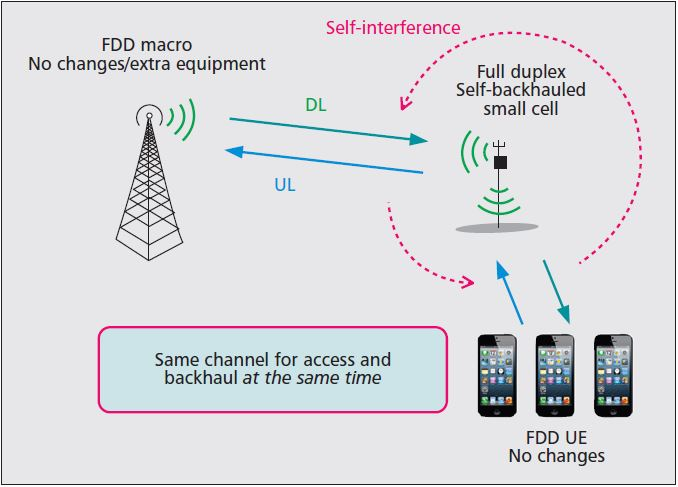
\includegraphics[width=\linewidth]{Kapitel/5G/Grafiken/sic}
\captionof{figure}{Nutzung von gleichen Frequenzen für Uplink und Downlink durch Mobilfunknetzzelle ~\cite{5g.7}}
\label{fig:5g.sic}
\end{Figure}

Die beste Ausnutzung des Frequenzspektrums kann nur mithilfe von Vollduplex (IBFD = In Band Full Duplex) erreicht werden, das heißt, dass zeitgleich auf der gleichen Frequenz gesendet und empfangen wird.
Unter Ausnutzung von IBFD kann also das Frequenzspektrum doppelt so effektiv genutzt werden wie bisher. Damit einher geht direkt, dass sich die Menge der übertragbaren Daten auf den Frequenzbereich hin betrachtet, sprich die Kapazität des Netzes, ebenfalls verdoppelt.
IBFD wurde im September 2015 zum ersten Mal von der Telekom durch die Nutzung von Selbstinterferenzunterdrückung (SIC = Self Interference Cancellation) erreicht.

Im Fall in Abbildung \ref{fig:5g.sic} wird SIC dadurch erreicht, dass die Netzzelle auf einer Frequenz vom Funkmast Daten erhält und auf dieser auch Daten an die einzelnen Endgeräte sendet. Zeitgleich empfängt sie auf einer zweiten Frequenz von den Endgeräten Daten und sendet auf dieser Daten auch an den Funkmast, sodass die Interferenz aufgehoben wird.

\begin{Figure}
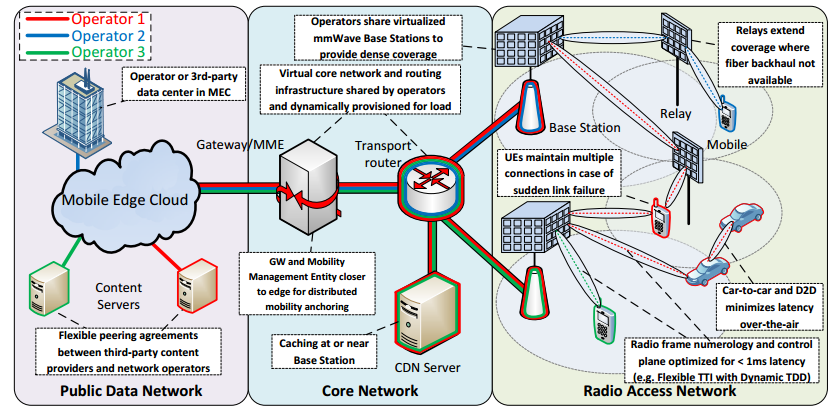
\includegraphics[width=\linewidth]{Kapitel/5G/Grafiken/5g-changes}
\captionof{figure}{Notwendige Veränderung am Netzwerk für möglichst geringe Latenzzeiten ~\cite{5g.9}}
\label{fig:5g.changes}
\end{Figure}


Um Latenzzeiten von weniger als \SI{1}{\milli\second} zu erreichen, müssen Vorkehrungen am gesamten  Netzwerk vorgenommen werden. Diese sind in Abbildung \ref{fig:5g.changes} aufgezeigt.
Darüber hinaus ist geplant einen höheren Frequenzbereich für die Datenübertragung zu verwenden als bisher. Dieser könnte im Bereich der Millimeter-Wellen liegen, also zwischen \SI{20}{\giga\hertz} und \SI{80}{\giga\hertz}.
Dadurch ist es möglich kritische Zeit bei der Datenübertragung und dem Datenempfang einzusparen
\subsection*{Einsatzmöglichkeiten}
Die Einsatzmöglichkeiten von 5G hängen besonders von 3 Eigenschaften des Netzwerks ab:
\begin{itemize}
\item Anzahl der maximalen Verbindungen
\item Latenzzeit
\item Übertragungsgeschwindigkeit
\end{itemize}

Dabei stellen einige Anwendungen ganz spezielle Anforderungen an das Netzwerk und die Technik, während andere weniger harte Kriterien aufweisen.

Wie auch aus Abbildung \ref{fig:5g.aw} hervorgeht, ist die Anzahl der Verbindungen die hauptsächlich definierende Größe, wenn es um Thematiken wie das Internet der Dinge und den zunehmenden Einsatz von Sensoren, auch im privaten Umfeld, geht.
Hier muss jedes Gerät stets mit dem Netzwerk in Verbindung stehen, um möglichst selbstständig präzise Entscheidungen treffen zu können. Somit wären elektrische Geräte in der Lage eigene Entscheidungen aufgrund dieser Sensoren zu treffen und zum Beispiel ein Kühlschrank in der Lage Informationen über seinen Inhalt vermitteln.

\begin{Figure}
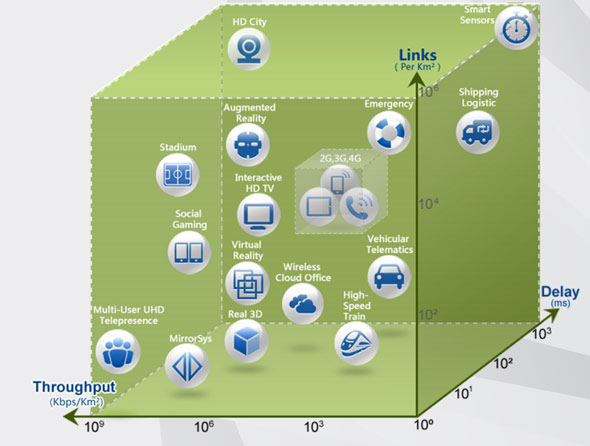
\includegraphics[width=\linewidth]{Kapitel/5G/Grafiken/5g-anwendung}
\captionof{figure}{5G-Anwendungswürfel von Huawei ~\cite{5g.6}}
\label{fig:5g.aw}
\end{Figure}

Auch beim Einsatz von Sensoren im privaten Umfeld, das heißt speziell die Überwachung der Körperfunktionen und Umgebung eines Nutzers, muss jeder Sensor in Echtzeit in Kontakt stehen mit beispielsweise dem Smartphone oder einem zentralen System, welches die Daten dann sammeln und auswerten könnte. Damit könnten frühzeitig drohende Gefahren für die Gesundheit wie Herzinfarkte erkannt werden. Darüber hinaus könnten mit den Sensordaten auch Hinweise zu einer gesünderen Lebensweise gegeben werden, um etwa Mineralmangel vorzubeugen, oder der Schlafrhythmus könnte entsprechend der Schlafphasen optimiert werden.

Um 5G auch als großflächiges Mobilnetzwerk nutzen zu können, werden bald neue Übertragungsgeschwindigkeiten notwendig sein. Wenn Videos in 4K und 3D nicht mehr die Ausnahme sind oder Nutzer die Vorteile von Virtual Reality (VR) im Alltag ausnutzen wollen, dann werden die aktuellen Geschwindigkeiten schnell an ihre Grenzen stoßen.
Beispielsweise benötigt das Bild, um echte VR zu erreichen, mindestens so viele Daten, wie die menschliche Retina erfassen kann. Um dies zur Verfügung zu stellen, werden über \SI{300}{\mega bit/\second} benötigt, was 4G-Netze schlicht nicht leisten können.
Durch Nutzung dieser Technik wäre es möglich virtuelle Klassenräume deutlich auszubauen. Dies könnte vor allem für Kinder in fern liegenden Gebieten eine große Hilfe sein.

Wenn vom Netz eine Latenzzeit von weniger als \SI{1}{\milli\second} gewährleistet werden kann, werden dadurch neue Möglichkeiten in der Automobiltechnik und der Medizin gegeben sein.

In der Automobiltechnik sind die Latenzzeiten von so hoher Bedeutung, da sich ein selbstfahrendes Auto unter Nutzung des aktuellen 4G-Netzes mit Latenzen von \SI{50}{\milli\second} bei \SI{100}{\kilo\metre /\hour} noch \SI{1.4}{\metre} bewegen würde, bevor es zu bremsen beginnt. Mit der angestrebten Latenzzeit von 5G könnte diese Strecke auf \SI{2.8}{\centi\metre} reduziert werden, was mit der Reaktionsgeschwindigkeit des ABS vergleichbar ist.

Außerdem könnten die einzelnen Fahrzeuge direkt miteinander in Kommunikation stehen, und sich so gegenseitig auf Gefahren aufmerksam machen oder melden, dass sie jetzt bremsen, wie in Abbildung \ref{fig:5g.c2c}.
\end{multicols}
\newpage
\section*{Historische Entwicklung}
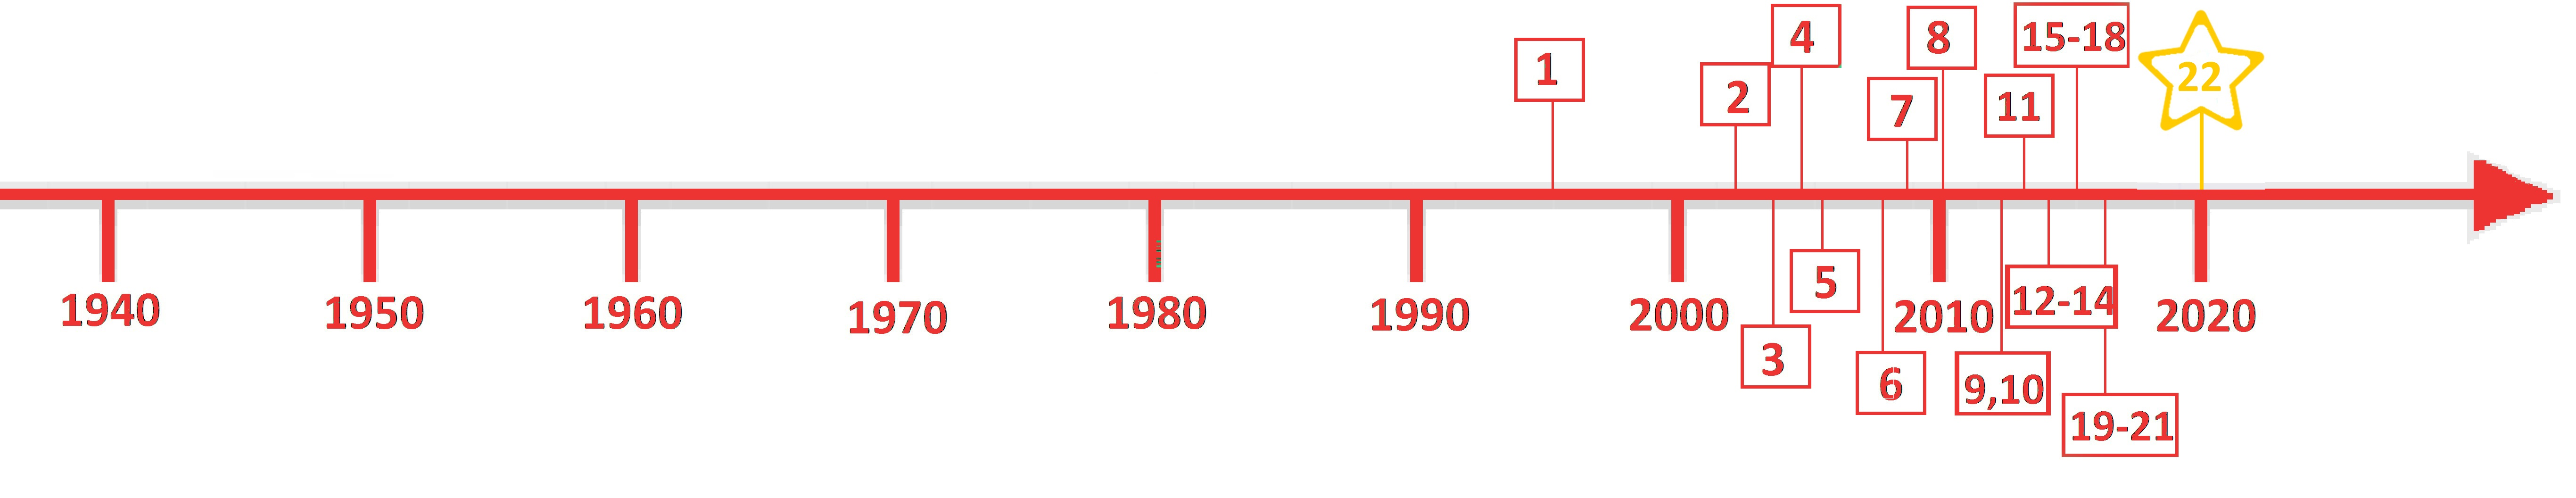
\includegraphics[width=\textwidth]{Kapitel/5G/Grafiken/Zeitstrahl2}
\par
\noindent
\begin{tabular}{p{1 cm}p{3 cm}p{13.55 cm}}
\rowcolors{2}{}{\topicolor!20}
	Nr. & Datum & Entwicklungsschritte~\cite{5g.1}\\
	1 & 1996 & 2G GSM \\
	2 & 2002 & Bekanntgabe der strategischen Vision für 4G\cite{5g.5} \\
	3 & 2004 & 3G UMTS\\
	4 & Anfang 2005 & Beginn der Standardisierung von 4G\cite{5g.5} \\
	5 & 2006 & 3G HSPA\\
	6 & 2008 & Die ersten Entwicklungsgruppen für 5G Mobilkommunikationssysteme werden gebildet.\\
	7 & 2009 & Das erste kommerzielle 4G-Netz wird von Ericsson und TeliaSonera in Betrieb genommen. \\
	8 & 2010 & 4G LTE großflächig verbreitet \\
	9 & 8. Oktober 2012 & Es erfolgt die Gründung eines 5G Forschungszentrums an der Universität in Surrey, Großbritannien. \\
	10 & November 2012 & Das \textit{iJOIN}-EU-Projekt zur Erforschung der besseren Ausnutzung des Spektrums wird gestartet. \\
	11 & 12. Mai 2013 & Samsung verkündet, das erste 5G-System entwickelt zu haben, welches Geschwindigkeiten bis zu 10Gbit/s erreichen können soll. Im Test wurde bei einer Reichweite von 2km eine Geschwindigkeit von 1.056Gbit/s erreicht. \\
	12 & 8. Mai 2014 & NTT DoCoMo beginnt 5G-Tests in Kooperation mit Alcatel, Ericsson, Fujistu, NEC, Nokia und Samsung. \\
	13 & Oktober 2014 & Das Projekt TIGRE5-CM wird gestartet, um die Architektur von künftigen Mobilfunknetzen auf Basis von SDN-Paradigmen (Software-defining networking) zu entwerfen. \\
	14 & November 2014 & Huawei und Megafon beginnen in Russland mit der Entwicklung eines 5G-Netzwerkes. Ein Testnetz soll bis Ende 2017 entstehen. \\
	15 & März 2015 & Vorstellung erster Ergebnisse des iJOIN-Projektes auf dem Mobile World Congress 2015 \\
	16 & September 2015 & Das 3rd Generation Partnership Project, kurz 3GPP, hält eine Konferenz zur Diskussion über die Entwicklung eines 5G-Standards ab. \\
	17 & 8. September 2015 & Verizon gibt bekannt, dass 2016 erste Tests von 5G in den USA beginnen sollen. \\
	18 & 28. September 2015 & Telekom gibt bekannt, dass ein erster Test mit SIC erfolgreich war, sodass zum ersten Mal IBFD erreicht wurde. \cite{5g.2} \\
	19 & 22. Januar 2016 & Ericsson und TeliaSonera geben erneut eine Zusammenarbeit bekannt. Sie wollen 2018 in Stockholm, Schweden und in Tallinn, Estland, die ersten 5G-Services anbieten. \\
	20 & 22. Februar 2016 & Samsung und Verizon geben ihre Zusammenarbeit bei 5G-Tests bekannt. \\
	21 & 23. Februar 2016 & Telekom führt auf dem Mobile World Congress 2016 einen 5G-Prototypen mit einer Geschwindigkeit von 1,5Gbit/s und weniger als 1ms Latenzzeit vor. \cite{5g.4}\\
	22 & 2020 & geplantes großflächiges Einführungsjahr dieser Technik \\
\end{tabular}
\par
\begin{multicols}{3}
\begin{Figure}
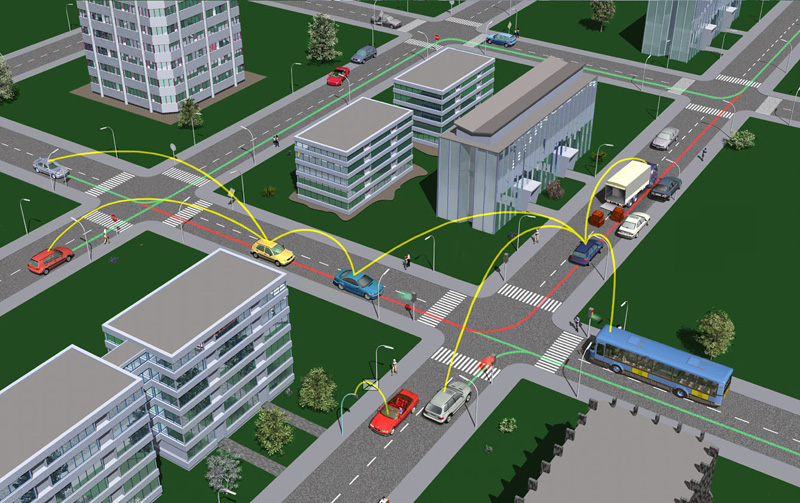
\includegraphics[width=\linewidth]{Kapitel/5G/Grafiken/c2c}
\captionof{figure}{3D Car-2-Car-Scenario von BMW ~\cite{5g.11}}
\label{fig:5g.c2c}
\end{Figure}

In der Medizin könnten diese Latenzzeiten in Kombination mit extrem präziser VR ermöglichen, dass spezialisierte Ärzte Operationen ausführen, obwohl sie sich an einem vollkommen anderen Ort in der Welt befinden. Dies kann zum Beispiel bei besonders schweren und komplizierten Operationen genutzt werden, die nur von wenigen Chirurgen präzise beherrscht werden.\cite{5g.10}
\subsection*{Ausblick}
Wenn wir den Ankündigungen der führenden Firmen glauben, so soll 5G ab 2020 im Einsatz sein. Ab der Gründung des ersten Forschungszentrums für diese Technik wären zu diesem Zeitpunkt also 8 Jahre vergangen.
Dies entspricht auch der Zeit, die es bei 4G von der strategischen Version 2002 bis zum Praxisbetrieb 2010 benötigt hat, weshalb es durchaus realistisch ist, dass 5G tatsächlich 2020 einsatzbereit ist. 
Mit dem Aufkommen von 5G stehen dann sowohl der Wirtschaft, in Bereichen wie Smart Logistics, als auch dem Endverbraucher, durch Dinge wie selbstfahrende Autos und Health Monitoring, ganz neue Möglichkeiten zur Verfügung, die das Leben verbessern können.

\printbibliography[segment=10,heading=subbibliography]
\end{multicols}

\newpage

\rowcolors{1}{}{}% TODO
%
% Steckbrief
% History
%

\begin{multicols}{3}[\section{IrDA}]

\rhead{Autor: Elias Holzmann}
\lfoot{Letzte Bearbeitung: 16.04.2016}

\newrefsegment

\begin{boxedminipage}{\linewidth}
\begin{tabular}{p{2,1 cm}p{2.7 cm}}
\textbf{Steckbrief}& \\
\end{tabular}
\begin{tabular}{p{2,1 cm}|p{2.7 cm}}
      Einsatz seit & 1993\\
      \hline
      Wellenlänge  & 850 - 900 nm\\
      \hline
      Datenrate & 2,4 kbit/s - 10 Gbit/s (noch in Entwicklung) \\
      \hline
      Einsatzzweck & Datenübertragung von und zu mobilen Geräten \\
\end{tabular}
\end{boxedminipage}
\par
%Source http://www.fh-bingen.de/fileadmin/user_upload/Lehrende/Kilsch_Dieter/internet/projekte/TedoSchStiUnits.pdf -> Seite 9 findet ihr alle verwendbaren Einheiten, wie:
%\SI{Zahl}{\mega\hertz} oder \SI{Zahl}{\mili\metre}
%Ich weiß ehrlich gesagt nicht welche Einheiten ihr im Text genau braucht, aber in dem Dokument und mit obigen Beispiel sollte es umsetzbar ein.
\subsection*{Überblick}
\begin{Figure}

\includegraphics[width=\linewidth]{Kapitel/IrDA/Grafiken/logo_irda.png}
\captionof{figure}{Logo der Infrared Data Association~\cite{irda}}
\label{fig:irda.logo}
\end{Figure}
Die IrDA (\textit{\textbf{I}nfra\textbf{r}ed \textbf{D}ata \textbf{A}ssociation}) ist eine 1993 gegründete Vereinigung.
Zur damaligen Zeit war Bluetooth noch nicht im Einsatz, die Datenübertragung zwischen PDAs, Notebooks und anderen mobilen Geräten erfolgte über proprietäre Protokolle, meist via Infrarot (\textit{\textbf{IR}}). Die IrDA hatte das Ziel, ein Protokoll zur Datenübertragung zu definieren, das die folgenden Bedingungen erfüllt:
\begin{itemize}
	\item offen, interoperabel
	\item kosteneffizient
	\item angemessen für eine großen Anzahl von Endgeräten~\cite{irdamarketing}
\end{itemize}

Aufgrund des Ziels der Kosteneffizienz wurde IR als Medium gewählt. Hierdurch sind nur eine LED und eine Photodiode notwendig, um einen Transceiver zu fertigen.~\cite{hparticle}

\subsection*{Technische Erläuterungen}
\begin{Figure}
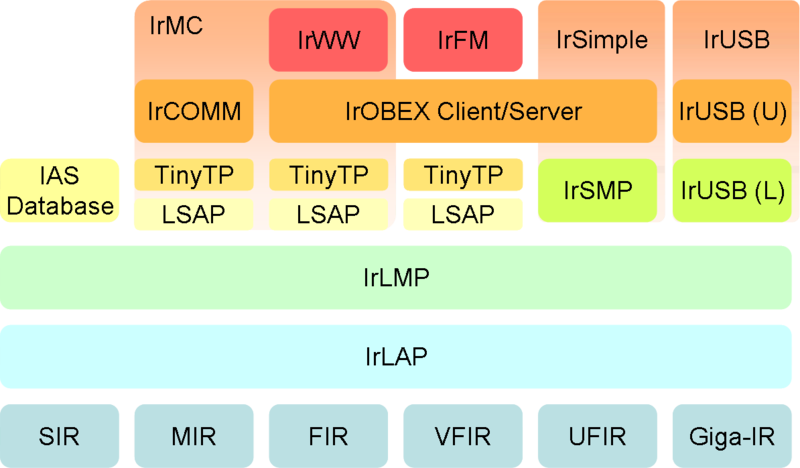
\includegraphics[width=\linewidth]{Kapitel/IrDA/Grafiken/protocol_stack.png}
\captionof{figure}{Übersicht über das IrDA-Protokoll~\cite{wikipediaen}}
\label{fig:irda.stack}
\end{Figure}
Die IrDA hat nicht wirklich ein einzelnes Protokoll spezifiziert, sondern vielmehr eine Protokollfamilie, vergleichbar mit dem TCP/IP-Protokollstack. In den folgenden Abschnitten werden die einzelnen Protokolle näher erläutert.
\subsubsection*{IrPHY}

\begin{Figure}
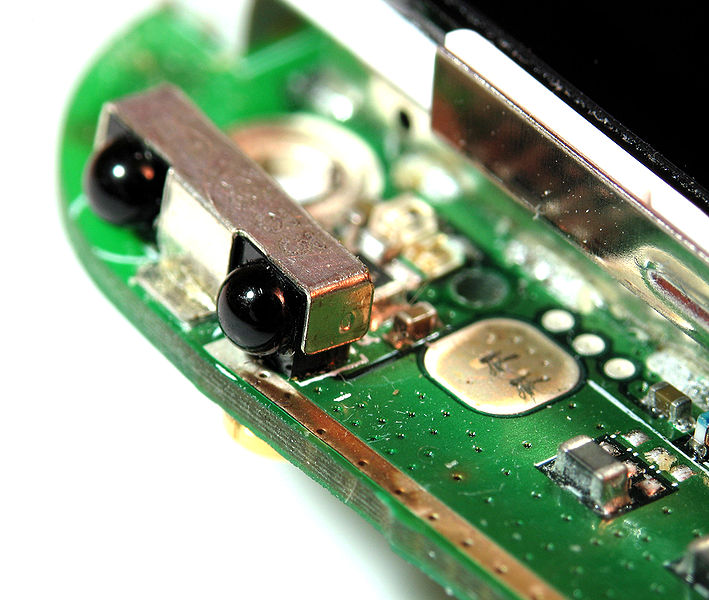
\includegraphics[width=\linewidth]{Kapitel/IrDA/Grafiken/irda_trans.jpg}
\captionof{figure}{Nahaufnahme eines IrDA-Transceivers, bestehend aus LED und Fotodiode.~\cite{wikipediade}}
\label{fig:irda.transceiver}
\end{Figure}
IrPhy (\textit{\textbf{I}nfra\textbf{r}ed \textbf{P}hysical \textbf{L}ayer \textbf{S}pecification}) arbeitet auf Schicht 1 des OSI-Modells, dem Physical Layer. Es definiert die physikalischen Eigenschaften der IR-Verbindung, wie Modulationsart und Kodierung.

Daten werden kodiert und über die IR-LED ausgegeben. Der Empfänger erhält diese Daten über die Fotodiode. Somit ergeben LED und Fotodiode einen Transceiver, wie er in Abbildung \ref{fig:irda.transceiver} dargestellt ist.

Für verschiedene Übertragungsgeschwindigkeiten werden unterschiedliche Varianten des Protokolls genutzt, die verschiedene physikalische Eigenschaften vorsehen. Aus diesem Grund wird an dieser Stelle nicht genauer auf die Definition eingegangen.

Die momentan eingesetzten Varianten sind, aufsteigend geordnet nach Geschwindigkeit:

\begin{itemize}
	\item SIR (Serial Infrared) - 9,6-115,2 kbit
	\item MIR (Medium Infrared) - 0,576-1,152 Mbit/s
	\item FIR (Fast Infrared) - 4 Mbit/s
	\item VFIR (Very Fast Infrared) - 16 Mbit/s
	\item UFIR (Ultra Fast Infrared) - 96 Mbit/s
	\item GigaIR - 1Gbit/s~\cite{wikipediaen}
\end{itemize}

Seit 2011 befindet sich eine weitere Variante des Protokolls namens 5/10GigaIR in Entwicklung, welche Übertragungsgeschwindigkeiten von 5 oder 10Gbit/s zulassen soll~\cite{irdagiga}. Jedoch sind hierüber und über den Fortschritt des Projekts kaum Informationen auffindbar.

Hardwareseitig wird zur Datenübertragung via IrDA lediglich eine Infrarot-LED zum Senden beziehungsweise eine Photodiode zum Empfangen der Daten benötigt. Dies ermöglicht die kostengünstige Fertigung von IR-Modems.
\subsubsection*{IrLAP}
IrLAP (\textit{\textbf{I}nfra\textbf{r}ed \textbf{L}ink \textbf{A}ccess \textbf{P}rotocol}) arbeitet auf Layer 2 des OSI-Modells, dem Data Link Layer. Es ist für die Discovery von Verbindungspartnern zuständig und stellt eine zuverlässige Verbindung bereit.

Zu diesem Zweck handelt IrLAP einen primären und einen sekundären Kommunikationspartner aus. Der sekundäre Kommunikationspartner darf erst senden, nachdem der primäre Kommunikationspartner dies erlaubt. Hierdurch werden Kollisionen verhindert.
\subsubsection*{IrLMP}
IrLMP (\textit{\textbf{I}nfra\textbf{r}ed \textbf{L}ink \textbf{M}anagement \textbf{P}rotocol}) ist Layer 4 des OSI-Modells zugeordnet, dem Network Layer. Es stellt mehrere logische Kanäle zur Verfügung, die über den selben physikalischen Link kommunizieren.
\subsubsection*{IrLAN}
IrLAN (\textit{\textbf{I}nfra\textbf{r}ed \textbf{L}ocal \textbf{A}rea \textbf{N}etwork}) liegt über IrLMP und erlaubt es, IrDA-fähige Endgeräte mit Token Ring- sowie Ethernet-Netzwerken zu verbinden.

\subsubsection*{Protokolle auf Anwendungsebene}
Die IrDA hat auch eine Vielzahl von Anwendungsprotokollen spezifiziert. Beispiele hierfür sind:
\begin{enumerate}
	\item OBEX (\textit{\textbf{Ob}ject \textbf{Ex}change}) erlaubt den Austausch von Dateien. Das Protokoll ist mittlerweile auch Teil des Bluetooth-Stacks.
	\item IrCOMM (\textit{\textbf{I}nfra\textbf{r}ed \textbf{Comm}unications Protocol}) emuliert eine serielle oder parallele Schnittstelle.
\end{enumerate}

\end{multicols}
\newpage
\section*{Historische Entwicklung}
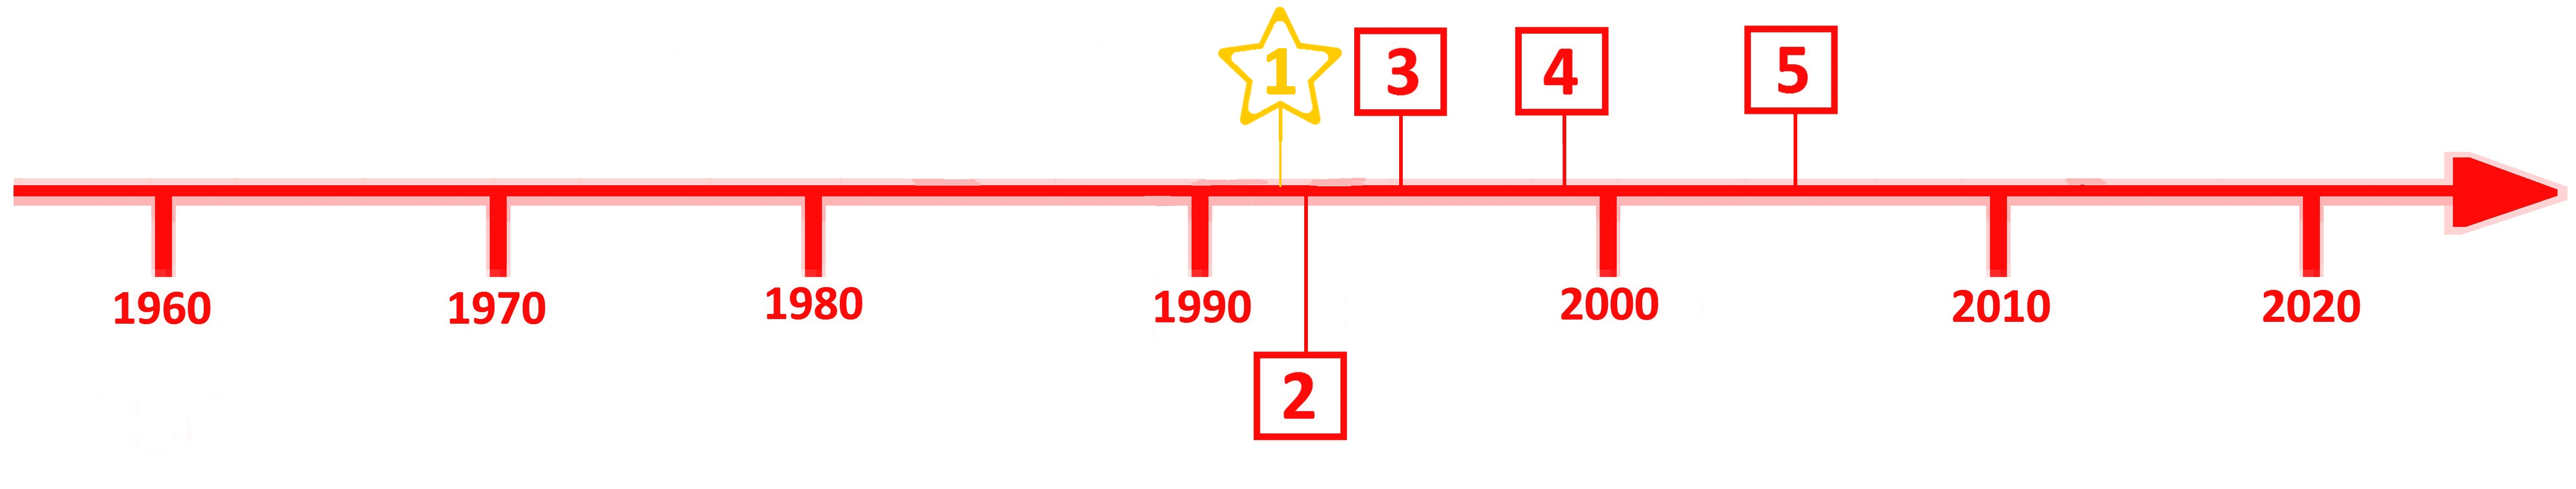
\includegraphics[width=\textwidth]{Kapitel/IrDA/Grafiken/Zeitstrahl.jpg}
\par
\noindent
\begin{tabular}{|p{1 cm}|p{3 cm}|p{13.55 cm}|}
	\hline
	Nummer & Datum & Entwicklungsschritte\\
	\hline
	1 & 1993 & Die Infrared Data Association wird gegründet.~\cite{wikipediade}\\
	\hline
	2 & 1994 & IrDA 1.0 wird veröffentlicht. Der Standard entthält die Spezifikation von SIR, IrLAP und IrLMP.~\cite{irdahistory}\\
	\hline
	3 & 1995 & IrPHY wird um MIR und FIR erweitert.~\cite{irdahistory}\\
	\hline
	4 & 1999 & IrPHY wird um VFIR erweitert.~\cite{irdahistory}\\
	\hline
	5 & 2005 & IrSimple wird spezifiziert.~\cite{wikipediade}\\
	\hline
\end{tabular}
\par
\begin{multicols}{3}

\subsection*{Einsatz}
\begin{Figure}
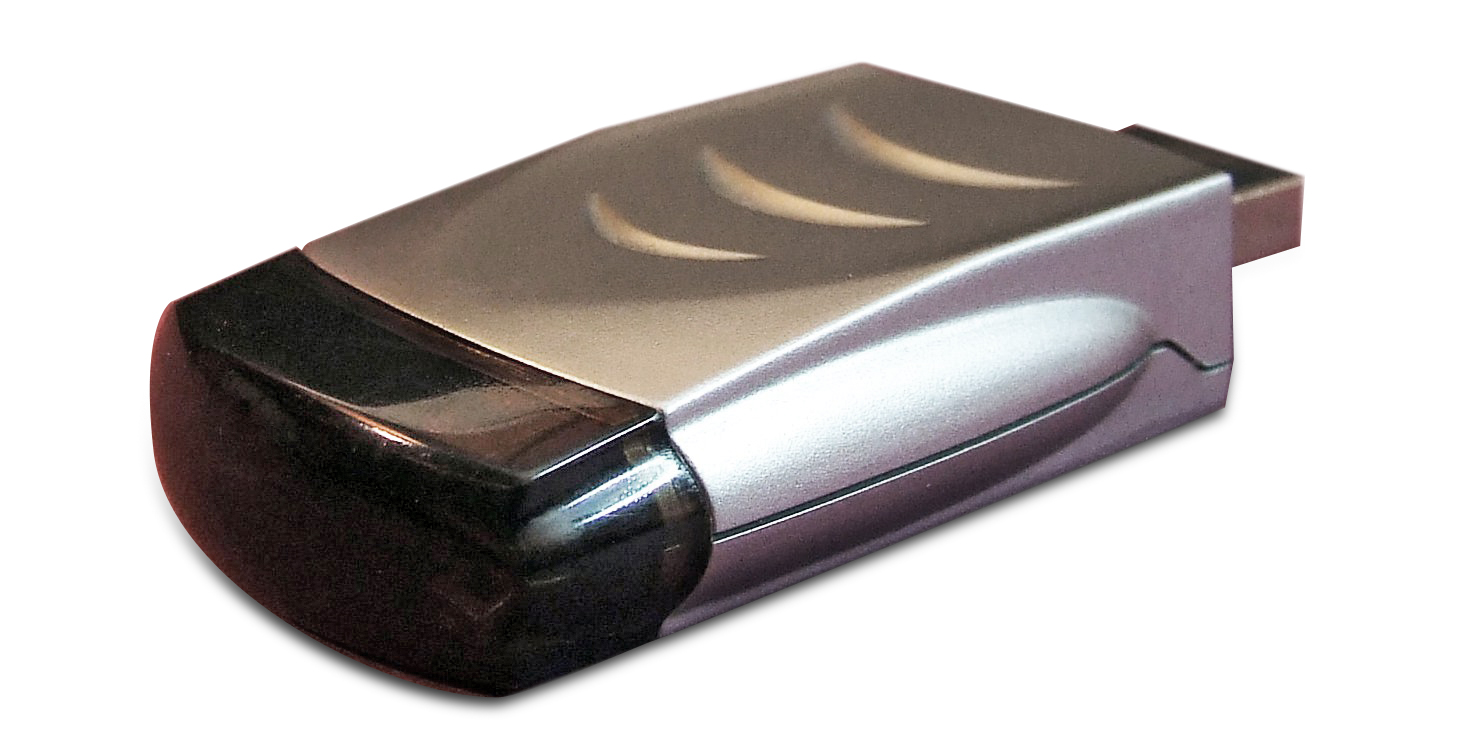
\includegraphics[width=\linewidth]{Kapitel/IrDA/Grafiken/irda_usb.jpg}
\captionof{figure}{Infrarot-USB-Modem für den PC~\cite{wikipediade}}
\label{fig:irda.modem}
\end{Figure}
Die IrDA-Protokollfamilie war rund um das Jahr 2000 weit verbreitet und wurde unter anderem auf PDAs, Notebooks und Handys im privaten und Enterprise-Umfeld eingesetzt.

Anfang der 2000er wurde IrDA und allgemein die Übertragung von Daten via IR mehr und mehr von Technologien auf Basis von Radiowellen, in erster Linie Bluetooth, verdrängt. Grund für diese Entwicklung war die Notwendigkeit, die Geräte für eine Übertragung via IR korrekt auszurichten. Bluetooth besitzt diese Einschränkung nicht nicht und ist daher anwenderfreundlicher. 

2005 gab es nochmals Versuche, IrDA mit den Weiterentwicklungen IrSimpleShot wiederzubeleben. IrSimple sollte dazu dienen, das Protokoll performanter zu gestalten, indem der Discovery-Prozess beschleunigt sowie die Datenrate erhöht wurde. IrSimpleShot ist ein Protokoll auf Basis von IrSimple zur Übertragung von Fotos. Es sollte dazu dienen, Fotos von einer Kamera schnell zur genaueren Betrachtung auf ein Anzeigegerät zu übertragen. Ziel war die Übertragung innerhalb einer Sekunde.

Nach Meinung des Autors war IrSimple größtenteils erfolglos, IrDA-fähige Geräte sind immer noch ein Nischenprodukt. 

\subsection*{Anbieter und Gremien}
IrDA, das Gremium, welches die vorgestellten Protokolle definiert hat, hatte zu seiner Hochzeit circa 50 Mitgliedsunternehmen, darunter Microsoft, HP und IBM. Heute besitzt die IrDA nur noch ca. 25 Mitglieder und veröffentlicht sehr viel seltener neue Spezifikationen als früher.

Alle von der IrDA erstellten Dokumente stehen den Mitgliedern kostenlos zur Verfügung. Nichtmitglieder müssen die Spezifikationen erwerben. Beispielsweise sind die sogenannten IrDA Core Specifications, also die Spezifikation der transportorientierten Protokolle wiebeispielsweise IrPHY, IrLAP und IrLMP, zusammen für 670 \$ erhältlich.

Eine Mitgliedschaft kostet zwischen 1500 \$ und 8000 \$ jährlich. Faktoren für die Kostenberechnung sind einerseits die Frage, ob das Mitglied Stimmrechte innerhalb der Organisation hat, und andererseits der jährliche Gewinn des Unternehmens.

\subsection*{Ausblick}
Die IrDA-Protokollfamilie wird wohl nicht mehr allzu lange weiterentwickelt. Zwar sind momentan noch Entwicklungen an 5/10GigaIR im Gange, jedoch dauern diese mittlerweile schon 5 Jahre an. Ob hier noch Ergebnisse zu erwarten sind, ist fraglich.

Microsoft hat mit Windows 10 auch den Support für den hauseigenen IrDA-Protokollstack eingestellt. Hierdurch können viele der Infrarot-Transceiver, die unter älteren Windows-Versionen noch funktionsfähig waren, nun nicht mehr genutzt werden. 

Durch diese und ähnliche Entwicklungen wird die Technologie wohl mittel- bis langfristig aussterben. Es erscheint höchst unwahrscheinlich, dass sich die Zahl der Nutzer nochmals erholt.

\printbibliography[segment=11,heading=subbibliography]
\end{multicols}

\newpage

\rowcolors{1}{}{}\begin{multicols}{3}[\section{NFC}]

\rhead{Mirko Grothe, Jan Selig}
\lfoot{14.05.2016}

\newrefsegment

\begin{tabular}{p{2,1 cm}p{2.7 cm}}
\textbf{Steckbrief}& \\
\end{tabular}
\begin{tabular}{p{2,1 cm}p{2.7 cm}}
\rowcolors{1}{\topicolor!20}{}
      Einsatz seit & 2002\\
      Frequenz"-bereich  & \SI{13.56}{\mega\hertz}\\
      Datenrate & \SI{424}{kBit/s}\\
      Verbreitung & gering\\
      Reichweite & \SI{4}{cm}\\
      Entwickelt von & Sony und Philips \\
      Spezifiziert durch & NFC Forum \\
      Technologie & RFID \\
      Standardisierung & ISO/IEC 18000-3 \\
      Modulation & Phasen Jitter Modulation \\
\end{tabular}
\par


\subsection*{Überblick}
\begin{wrapfigure}{r}{0.4\linewidth} 
\vspace{-20pt} 
\begin{center} 
\hspace{-20pt} 

\includegraphics[width=0.7\linewidth]{Kapitel/NFC/Grafiken/Logo.jpg} 
\end{center} 
\vspace{-15pt} 
\end{wrapfigure} 


\textbf{N}ear \textbf{F}ield \textbf{C}ommunication\footnote{NFC {http://nfc-forum.org//}} (z.dt. Nahfeldkommunikation, Abkürzung NFC) ist ein internationaler Übertragungsstandard zum kontaktlosen Austausch von Daten zwischen zwei Geräten. Aufgrund der geringen Reichweite und der niedrigen Übertragungsrate ist NFC nicht für das Senden umfangreicher Daten geeignet. Stattdessen ist NFC auf Dienste ausgelegt, bei denen ein Transfer geringer Datenmengen über kurze Reichweiten initiiert wird, ohne das bei jedem Verbindungsaufbau eine zeitintensive Kopplung erforderlich ist.
Die Datenübertragung ist intuitiv und kann daher bei entsprechender Konfiguration automatisch gestartet werden, sobald ein NFC fähiges Gerät in Reichweite ist.~\cite{nfc.1,nfc.2,nfc.12}


\subsection*{Technische Erläuterungen}
NFC wurde gezielt für eine Übertragung geringer Datenmengen mit schnellem Verbindungsauf und -abbau entwickelt. Dies wird realisiert, indem der Datentransfer zwischen zwei NFC fähigen Geräten automatisch initiiert wird, sobald diese in Reichweite sind. Um unbeabsichtigte Verbindungen oder ein Abhören der zu übermittelnden Daten zu verhindern, ist die Übertragung mit NFC nur in geringer Reichweite im Zentimeterbereich möglich. Damit kann eine Kontaktaufnahme als Zustimmung zu einer Datentransaktion gewertet werden. Bei sicherheitskritischen Transaktionen wie Kreditkartenzahlungen erfolgt die Kommunikation zusätzlich verschlüsselt.

Jedes NFC Gerät unterstützt zwei Betriebsmodi. Im \textit{passiven Modus} wird das Senden und Empfangen von Daten von einem anderen aktiven Gerät initiiert und gesteuert. Das passive Gerät kann hierbei ausgeschaltet sein. 
Im \textit{aktiven Modus} kann ein Gerät zusätzlich zur passiven Funktion einen Datentransfer selbst veranlassen. Sind beide Geräte im aktiven Modus, so spricht man auch vom sogenannten Peer-to-Peer-Modus, da ein Datenaustausch in Form eines Dialogs möglich ist. 

Des Weiteren gibt es sogenannte NFC Tags; diese besitzen im Gegensatz zu NFC Geräten keine eigene Stromversorgung und können äquivalent zu ausgeschalteten Geräten nur im passiven Modus arbeiten. Darüber hinaus können sie, anders als NFC Geräte, nicht gleichzeitig Daten senden und empfangen.

NFC nutzt die RFID Technologie (radio-frequency identification), die in Abb. \ref{fig:nfc.RFID} dargestellt ist. Diese ist ein Sender-Empfänger-System zum automatischen und berührungslosen Identifizieren von Objekten über Funkwellen mit einer Frequenz von 13.56~MHz~\cite{nfc.9}. Jedes NFC Gerät (nicht NFC Tags) kann sowohl die Rolle des Senders, als auch die des Empfängers übernehmen. Mit seiner Peer-to-Peer-Funktion grenzt sich NFC zur RFID Technologie ab, bei der nur eine Kommunikation zwischen aktivem Sender und passivem Empfänger möglich ist. 

\begin{Figure}
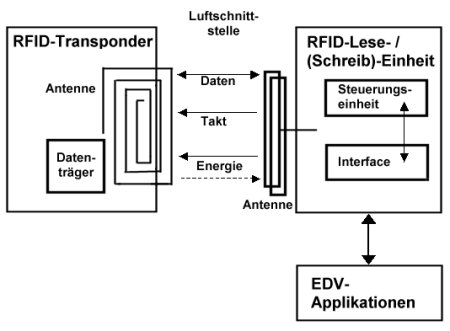
\includegraphics[width=\linewidth]{Kapitel/NFC/Grafiken/RFID.jpeg}
\captionof{figure}{RFID Technologie~\cite{nfc.13}}
\label{fig:nfc.RFID}
\end{Figure}

Ein anfragendes Gerät erzeugt mittels einer Spule ein elektromagnetisches Wechselfeld mit einer Trägerfrequenz von 13,56~MHz. Unterschreitet es dabei den maximalen Senderadius zu einem anderen Gerät, so induziert es über eine Spule im Stromkreis des empfangenden Gerätes eine Spannung. Weil das Magnetfeld aufgrund der Wechselspannung nicht konstant ist, fungiert es für das empfangende Gerät als konstante Energiequelle, solange letzteres sich innerhalb dessen Sendereichweite befindet. Aus diesem Grund kann ein Gerät im passiven Modus von seiner eigenen Energieversorgung getrennt sein und ein NFC Tag ohne eigene Energiequelle auskommen.

Über die sogenannte induktive Kopplung zwei benachbarter elektrischer Stromkreise erfolgt neben der Energieübertragung auch die Kommunikation der beiden Geräte. Die Daten werden über das Magnetfeld per Phasen Jitter Modulation von dem anfragenden Gerät an das empfangende Gerät gesendet. 

\begin{Figure}
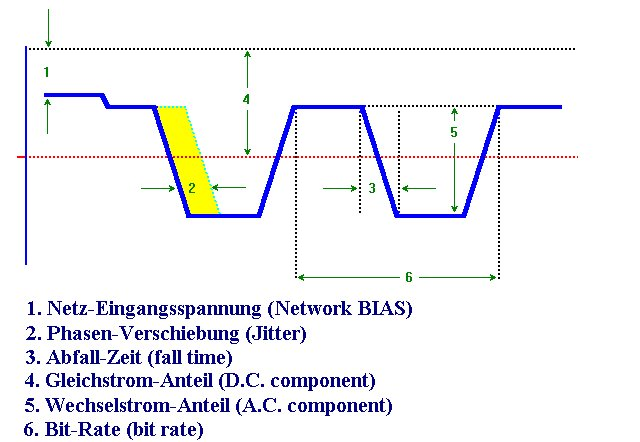
\includegraphics[width=\linewidth]{Kapitel/NFC/Grafiken/PJM.jpg}
\captionof{figure}{Phasen Jitter Modulation~\cite{nfc.14}}
\label{fig:nfc.PJM}
\end{Figure}

Die PJM (Abb. \ref{fig:nfc.PJM}) ist eine abgeschwächte Form der Phasenmodulation, bei der vom sendenden Gerät nur sehr kleine Änderungen an der Phase des Trägersignals vorgenommen werden. Während der unmodulierte Teil des Signals zur Energieversorgung des Empfängers dient, demoduliert und interpretiert dieser den geringen modulierten Anteil des Signals durch Vergleichen mit dem unmodulierten Anteil. 

Bei der Datenübertragung vom Empfänger zurück zum anfragenden Gerät bedient sich Ersterer der modulierten Rückstreuung. Hierbei reflektiert der Empfänger das empfangene Signal mit gleicher Trägerfrequenz und gleichzeitig veränderten Amplituden (Amplituden-Modulation). Dies wird durch kurzeitiges Ändern der Impedanz der Empfängerspule realisiert. Durch Demodulation und Interpretation der veränderten Amplituden des zurückgestreuten Signals erhält das anfragende Gerät die Antwort des empfangenden Gerätes.~\cite{nfc.3,nfc.4,nfc.5,nfc.6,nfc.7,nfc.8}


\subsection*{Einsatz}
\begin{itemize}
\item Kontaktlose Datenübertragung über kurze Distanzen
\item Potentielle Ablösung von Kreditkarten und Schlüsseln aufgrund eines schnellen Verbindungsaufbaus
\item Wasserdichte Konstruktionen der Geräte möglich
\item Mobile Payment zum kontaktlosen Bezahlen mit NFC fähigen Kreditkarten oder Smartphones
\item Schlüsselkarten zum Öffnen von Türen und Schranken
\item Digitale Eintritts- und Fahrkarten
\item Chips zur Arbeitszeiterfassung
\item Pairing zweier Geräte über Bluetooth
\item Bereitstellen von Terminals, die Informationen versenden~\cite{nfc.1,nfc.2,nfc.10}
\end{itemize}
\end{multicols}
\newpage

\section*{Historische Entwicklung}
\includegraphics[width=\textwidth]{Kapitel/NFC/Grafiken/Zeitstrahl2}
\par
\noindent
\begin{tabular}{p{0.5 cm}p{1.5 cm}p{15.55 cm}}
\rowcolors{2}{}{\topicolor!20}
	Nr. & Datum & Entwicklungsschritte~\cite{nfc.1}\\
	1 & 1983 & Das erste Patent mit der Abkürzung „RFID“ wird auf Charles Walton ausgestellt.\\
	2 & 2002 & Sony und Philips einigen sich auf eine technische Spezifikation.\\
	3 & 2004 & Nokia, Philips und Sony etablieren das Near Field Communication (NFC) Forum.\\
	4 & 2006 & Erste Spezifikation für NFC-Tags wird veröffentlicht.\\
	5 & 2006 & Nokia präsentiert das erste NFC-fähige Mobiltelefon.\\
	6 & 2009 & Das NFC-Forum veröffentlicht Peer-to-Peer-Standards.\\
	7 & 2012 & Einführung von girogo.\\
\end{tabular}
\par
\begin{multicols}{3}

\subsection*{Anbieter und Gremien}
Die 2002 von \textit{Philips} und \textit{Sony} entwickelte Nahfeldkommunikation wird durch die öffentliche Plattform \textit{NFC Forum} spezifiziert. Die Spezifikationen umfassen Standards für die Gerätearchitektur von NFC Geräten und die bei der Kommunikation verwendeten Protokolle.

Seit Anfang 2012 haben in Deutschland Kreditkarten von \textit{Visa} (payWave) und MasterCard (PayPass) einen NFC Chip verbaut. Damit können bei kooperierenden Händlern Beträge bis maximal 25 Euro ohne PIN Abfrage bezahlt werden. Sparkassen und Volksbanken bieten mit ihrer Girocard (girogo (Abb.~\ref{fig:nfc.girogo})) ebenfalls eine NFC Funktion zum kontaktlosen Bezahlen.
Studentenausweise, mit denen man kontaktlos bezahlen kann und auch der neue Personalausweis, enthalten in der Regel noch RFID- statt NFC Chips.

\begin{Figure}
\includegraphics[width=\linewidth]{Kapitel/NFC/Grafiken/girogo.jpg}
\captionof{figure}{Röntgenbild einer Girocard~\cite{nfc.1}}
\label{fig:nfc.girogo}
\end{Figure}

Bei modernen Multimedia Systemen ist NFC häufig bei Vorhandensein einer Bluetooth Funktion anzutreffen, um ein schnelles und kontaktloses Pairing mit einem anderen Bluetooth Gerät zu ermöglichen.~\cite{nfc.2,nfc.11,nfc.12}


\subsection*{Ausblick}
Als Studentenausweis mit Bezahlfunktion oder Schlüsselersatz für Mitarbeiter hat sich NFC bis heute nicht durchgesetzt, da hier die ältere RFID Technologie bereits weit verbreitet im Einsatz ist. Während der Übertragungsstandard im Mobile Payment mit Anbietern wie Google Wallet noch ein Nischendasein fristet, bieten die neuen Kreditkarten von Visa (payWave) und MasterCard (PayPass) bereits die Möglichkeit per NFC zu bezahlen. Bis dato unterstützen allerdings nur wenige Händler diese Zahlungsmöglichkeit.

In Zukunft wird NFC meiner Meinung nach vermehrt in der Praxis Anwendung finden, wie zum Beispiel das Ersetzen von Bezahlmitteln durch eine virtuelle Bankkarte, die eine Applikation in einem NFC fähigen Smartphone darstellt, oder das Ersetzen von Autoschlüsseln durch NFC fähige Smartphones.~\cite{nfc.2} Weiteres Potential besteht auch in Applikationen, die in Kombination mit sogenannten „NFC Stickern“ verwendet werden. Hierdurch ist es so zum Beispiel möglich NFC als eine Art Informationsvermittler zu verwenden, der Informationen bereitstellt, wenn das Smartphone in Reichweite des Stickers ist.~\cite{nfc.15}

\printbibliography[segment=12,heading=subbibliography]

\end{multicols}
\newpage


\renewcommand{\topicolor}{iot}
\renewcommand{\topicategory}{Home Automation/Internet of Things}
\rowcolors{1}{}{}\begin{multicols}{3}[\section{Bluetooth Low Energy}]

\rhead{Autor: Sven Guthe}
\lfoot{Letzte Bearbeitung: 16.04.2016}

\newrefsegment

\begin{boxedminipage}{\linewidth}
\begin{tabular}{p{2,1 cm}p{2.7 cm}}
\textbf{Steckbrief}& \\
\end{tabular}
\begin{tabular}{p{2,1 cm}|p{2.7 cm}}
      Einsatz seit & Dezember 2009\\
      \hline
      Frequenz"-bereich  & \SI{2,4}{\giga\hertz}-Band mit 40 Kanälen zwischen \SI{2,402}{\giga\hertz} und \SI{2,483}{\giga\hertz}\\
      \hline
      Datenrate & \SI{0,27}{Mbit/s}\\
      \hline
      Verbreitung & Weltweit (vor allem Smart Wearables)\\
      \hline
      Reichweite & \SI{10}{\metre}\\
\end{tabular}
\end{boxedminipage}
\par

\subsection*{Überblick}
Bluetooth Low Energy (BLE) ist eine Kabellose Übertragungstechnologie, welche für Datenübertragungen zwischen kurzen Entfernungen von der Bluetooth Special Interest (SIG) Group entwickelt wurde. Wie die Bezeichnung der Technologie preisgibt, handelt es sich um eine Bluetooth-Spezifikation, bei welcher der energiesparsame Betrieb im Vordergrund steht um Verbindungen zu Geräten mit kleinem Energiespeicher herzustellen. Mit dieser Entwicklung, sichert sich der Bluetooth-Standard Anteile vor allem in den aufstrebenden Märkten der Gesundheitsindustrie (Fitnesstracker) und der Unterhaltungselektronik (Kopfhörer).
Zur Anwendung kommt BLE in Wearables wie Smartwatches, in Notebooks, in Smartphones und in vielen weiteren Geräten~\cite{BLE.4}.

\begin{Figure}
\includegraphics[width=\linewidth]{Kapitel/BLE/Grafiken/Bluetooth_Smart_Logo.png}
\captionof{figure}{Bluetooth Smart Logo~\cite{BLE.2}}
\end{Figure}

\subsection*{Technische Erläuterungen}
Eine Bluetooth Verbindung basiert auf einer Kommunikation zwischen einem Master und einem Slave. Der Master ist dabei das Gerät, welches die Verbindung initiiert. Dieser stellt auf 40 Kanälen eine Verbindung zum Slave her und kann dank des Frequenzsprungverfahren auf allen Kanälen parallel Daten senden, wodurch die Bandbreite enorm erhöht wird. Als Konsequenz ergibt sich aber, dass der Master-Takt bei allen verbundenen Slaves synchronisiert werden muss.
Eine Verbindung des Masters zu mehreren Slaves (max. 7) wird als "Piconet" bezeichnet. Befindet sich ein Gerät in mehreren Piconets, wird dies "Skatternet" genannt. Bei diesen Netzen kommt es zusätzlich noch zur Abstimmung der jeweiligen Sendekanäle und der Reihenfolge, in welcher die Daten in das jeweilige Netz gesendet werden.

Wie auch bei der Datenübertragung per WLAN werden die zu übersendenden Daten in Pakete unterteilt und versendet. Dabei wird bei dem Bluetooth Standard unterschieden zwischen einer synchronen (SCO - Synchronous Connection Oriented) und in einer asynchronen (ACL - Asynchronous ConnectionLess) Übertragung. Für die BLE-Technologie ist dabei vor allem die asynchrone Übertragung von Interesse. Dabei werden Daten zu einem beliebigen Zeitpunkt über die Pico-Netzwerke versendet und können gegebenenfalls erneut angefordert werden.

Ein Asynchrones Paket bestehet aus einer Identifikationssequenz (68-72 Bit, Access Code) zur Identifikation für das aktuelle Piconet, aus der Adresse des Slaves (3 Bit, Logical Transfer Address), einer Information über den verwendeten Pakettyp (4 Bit, Packet Type), 3 Flags, welche für das Blockieren des Controllers (Flow), für die Information, ob das letzte Paket erfolgreich angekommen ist (Automatic Repeat Request Number) und einer Sequenznummer (SEQN), um zu überprüfen, ob die Reihenfolge eingehalten wurde. Außerdem wird ein Hashwert (8 Bit, Header Error Check) angefügt, um ein mögliches falsches Paket zu erkennen. Hinter dieser festgesetzten Folge von Bits folgen schließlich die eigentlichen Informationen (0-2744 Bits, wobei nochmals 32 Bits für konkrete Informationen zum Paket verloren gehen)~\cite{BLE.1}.

\begin{Figure}
\includegraphics[width=\linewidth]{Kapitel/BLE/Grafiken/paket.png}
\captionof{figure}{ACL Paket~\cite{BLE.1}}
\end{Figure}

Übertragen werden die Informationen auf Frequenzen zwischen 2,402 GHz und 2,483 GHz auf 40 Kanälen. Damit kommt es zwar zwischen BLE und anderen Funktechnologie zu Überlagerungen, allerdings wechselt BLE seinen Sendekanal bis zu 1600 mal pro Sekunde.
Um die Übertragung entsprechend zu modulieren, wird der GFSK (Gaussian Frequency Shift Keying) Standard eingesetzt, bei der die schnell und stark ansteigenden Flanken abgeflacht und somit die für die Übertragung weniger Bandbreite benötigt wird.

Für die Übertragung werden Protokolle verwendet, welche denen aus dem bekannten OSI-Modell entsprechen. Dabei kommen die Schichten des Physical Layers in Form des Radio Layers und der Data Link Layer in Form des Baseband und des Link Manager Layers zum Einsatz. 
Der Radio Layer moduliert und demoduliert das Signal sowie versendet bzw. empfängt physikalische Signale. Der Baseband Layer sorgt für die Kontrolle der angekommenen Daten und sendet, falls nötig, eine Aufforderungen zur erneuten Sendung von fehlgeschlagenen Paketen aus. Zuletzt analysiert und verwaltet der Link Manager alle Verbindungen und setzt eine Authentifizierung zwischen Master und Slave sowie eine Verschlüsselung um.

Bei der Authentifizierung lässt BLE die Möglichkeiten offen, ob diese stattfinden muss oder nicht. Mithilfe des Object Push Profile (OPP) können Daten gesendet werden ohne jegliche Authentifizierung. Am Slave-Gerät muss nur bestätigt werden die Daten anzunehmen. Allerdings entspricht dies nicht dem Normalfall.
Wie bei dem Serial Port Profile müssen sich Geräte vor einer Datenübertragung pairen. Dazu ist es notwendig, einen zuvor ausgehandelten PIN einzugeben. Nach erfolgreichem Pairing, wird das verbundene Gerät in einer Liste von bekannten Geräten angezeigt. Neben dem Einsatz von PINs, wird auch das Pairing per NFC (Near Field Communication) immer mehr zum Standard.

Das Spezielle an dem Bluetooth Low Energy Standard sind die Zeitintervalle und die Datenmenge welche an gekoppelte Geräte übertragen werden. Anders als bei allen anderen Bluetooth Standards ist, dass BLE auf den Geräten nicht dauerhaft eingeschalten ist, sondern nur in gewissen Zeitabständen relevante Informationen sendet. Außerdem ist auch die Datenübertragung in ihrem Umfang eingeschränkt. Es werden maximal 220 kBit/s übertragen. Dies bedeutet, dass BLE nicht für alle Anwendungen in Frage kommt und bei größeren Datenmengen doch auf andere Standards zurückgegriffen werden muss. Durch den Fokus auf den stromsparenden Verbrauch von Bluetooth, wird neben der Datenrate und den Zeitabständen auch die Reichweite stark eingeschränkt. Von rund 100 Metern bei "normalen" Bluetooth sind bei BLE lediglich 10 Meter zu erreichen~\cite{BLE.1}.

\subsection*{Einsatz}
Die Einsatzmöglichkeiten von BLE sind sehr breitgefächert. Dabei wird auf einzelne Anwendungsgebiete genauer eingegangen. Ein durchaus gewinnbringender Einsatz ist im Einzelhandel möglich. Dabei können Geräte des Kunden im Geschäft automatisch Kontakt zu einem Bluetooth Access Point aufnehmen und Informationen über den Kunden und dessen Kaufverhalten an die Verkäufer senden. Interessanten Informationen wären dabei Browserverläufe, bei denen sich der Kunde auf der Suche nach Mode befand, vorausgesetzt der Kunde befindet sich in einem Modegeschäft. Neben den Möglichkeiten, den Verkäufer mit relevanten Informationen zu versorgen, ist es natürlich ebenfalls möglich, dem vermeintlichen Käufer einen Überblick über den Laden zu geben und benötigte Kleidung zu lokalisieren.

Das aber vermutlich gewinnbringendste Gebiet für BLE ist die Gesundheitsbranche. Geräte zum Puls anzeigen, Schritte zu messen oder auch Sportaktivitäten aufzuzeichnen sind bereits überall in allen Preisklassen erhältlich. Aber die Branche wird noch viel weiter gehen. Warum sollten nicht auch detailliertere Informationen über den Zustand des Körpers ermittelt und an das Handy bzw. direkt ans zuständige Krankenhaus gesendet werden. Mit kleinen Sensoren, welche über BLE verfügen, wäre dies realisierbar und stellt auch für den Nutzer einen Mehrwert dar, da er sich jeder Zeit über den Zustand seines Körpers informieren kann.

Auch in der Industrie bei der Wartung von Maschinen ist ein Verwenden von Bluetooth von großem Vorteil. Damit wäre es möglich, Fehler unabhängig von der Maschine, mit einem einzelnen portablen Gerät (Handy) abzulesen. Dies würde die Unternehmen unabhängiger von teurer Software der Entwickler machen und könnten die Oberflächen, je nach Anwendungsbedarf, selbst modifizieren.

Wie schon durch die drei aufgelisteten Bei-

\end{multicols}

\section*{Historische Entwicklung}
\includegraphics[width=\textwidth]{Kapitel/BLE/Grafiken/Zeitstrahl}
\par
\noindent
\begin{tabular}{|p{1 cm}|p{3 cm}|p{13.55 cm}|}
	\hline
	Nummer & Datum & Information \\
	\hline
	1 & August 1993 & Gründung der Infrared Data Association (IrDA) mit dem Ziel ein einheitliches Protokoll für Datenübertragung über Infrarot bereitzustellen.\\
	\hline
	2 & 1998 & Gründung der Bluetooth Special Interest Group (SIG) durch die Firmen Ericsson, Nokia, IBM, Toshiba und Intel zur Ausarbeitung eines Standards, der verbindliche Spezifikationen festlegte.\\
	\hline
	3 & Juli 1999 & Bereitstellung der Spezifikation Bluetooth 1.0 (Juli) und Bluetooth 1.0b (Dezember).\\
	\hline
	4 & Februar 2001 & Bereitstellung der Spezifikation Bluetooth 1.1.\\
	\hline
	5 & November 2003 & Bereitstellung der Spezifikation Bluetooth 1.2.\\
	\hline
	6 & November 2004 & Bereitstellung der Spezifikation Bluetooth 2.0 + EDR.\\
	\hline
	7 & August 2007 & Bereitstellung der Spezifikation Bluetooth 2.1 + EDR.\\
	\hline
	8 & April 2009 & Bereitstellung der Spezifikation Bluetooth 3.0 + HS.\\
	\hline
	\textbf{9} & \textbf{Dezember 2009} & \textbf{Bereitstellung der Spezifikation Bluetooth 4.0.}\\
	\hline
	10 & Dezember 2013 & Bereitstellung der Spezifikation Bluetooth 4.1.\\
	\hline
	11 & Dezember 2014 & Bereitstellung der Spezifikation Bluetooth 4.2.\\
	\hline
\end{tabular}
\par
\begin{multicols}{3}

spiele zu erkennen ist, ist Bluetooth in allen Gebieten des Lebens verwendbar in denen Daten übertragen werden müssen. Durch das Entwickeln des BLE Standards ist man zudem unabhängiger von Entwicklungen in der Batterieindustrie und kann mittels kleiner Energievorräte, Daten an kompatible Geräte senden. Damit wird BLE nicht nur für Konsumenten einen Mehrwert darstellen, sondern auch in der Entwicklung des "Internet der Dinge" (IoT - Internet of Things) in Verbindung mit SmartHome und anderen Technologien~\cite{BLE.1}.

\subsection*{Anbieter und Gremien}
Das Gremium, welches für die Entwicklung für neue Bluetooth Technologien zuständig ist, ist die schon genannte Bluetooth Special Interest (SIG) Group. Gegründet wurde dieses Gremium 1998 von den Unternehmen Nokia, Toshiba, Intel, IBM und Ericsson. Bis zum Jahre 1999 stiegen auch 3Com, Motorola, Lucent und Microsoft in die SIG Gruppe ein. SIG besitzt das Warenzeichen von Bluetooth und bestimmt mit den Entwicklungen der neuen Standards auch deren Spezifikationen. Mittlerweile wird das SIG Gremium von mehr als 30.000 Mitgliedern unterstützt~\cite{BLE.1}.

\begin{Figure}
\includegraphics[width=\linewidth]{Kapitel/BLE/Grafiken/BluetoothSIGLogo.jpg}
\captionof{figure}{Bluetooth SIG Logo~\cite{BLE.3}}
\end{Figure}

\subsection*{Ausblick}
Einen kleinen Ausblick konnte man schon bei den Einsatzgebieten einsehen, in denen man erkennen konnte, wie wichtig Bluetooth in der zukünftigen Vernetzung wird. Neben den Anwendungsgebieten, welche mit besseren Eigenschaften natürlich auch weiter steigen, sind auch neue Standards mit höheren Übertragungsraten auch im Low Energy Bereich geplant. Damit wird der BLE Standard auch für Anwendungen, in denen mehr Datenvolumen übertragen werden muss, interessant.

Das größte, interessanteste aber auch unberechenbarste Gebiet der Entwicklung für Übertragungstechnologie wird aber das "Internet der Dinge" darstellen. In der immer schnelleren Vernetzung des eigenen Zuhauses, des Körpers und andere Dinge des täglichen Lebens werden Übertragungsmöglichkeiten zwischen den Sensoren immer wichtiger. Ob sich der Bluetooth Standard dabei durchsetzt ist aufgrund der Schnelllebigkeit in Gebieten der Technik allerdings nicht zu beurteilen~\cite{BLE.1}.

\printbibliography[segment=4,heading=subbibliography]
\end{multicols}

\newpage

\rowcolors{1}{}{}\begin{multicols}{3}[\section{IEEE 802.11 Basics}]

\rhead{Jan Selig, Simon Retzmann}
\lfoot{16.05.2016}

\newrefsegment

\begin{boxedminipage}{\linewidth}
\begin{tabular}{p{2,1 cm}p{2.7 cm}}
\textbf{Steckbrief}& \\
\end{tabular}
\rowcolors{1}{\topicolor!20}{}
\begin{tabular}{p{2,1 cm}p{2.7 cm}}
      Einsatz seit & 1997\\
      Frequenz"-bereich  & \SI{2.4}{\giga\hertz}, \SI{5}{\giga\hertz} \\
      Datenrate & \SI{2}{Mbit/s} - \SI{54}{Mbit/s}\\
      Verbreitung & Weltweit\\
      Reichweite & ca. \SI{20}{\metre}\\
\end{tabular}
\end{boxedminipage}
\par
%Source http://www.fh-bingen.de/fileadmin/user_upload/Lehrende/Kilsch_Dieter/internet/projekte/TedoSchStiUnits.pdf -> Seite 9 findet ihr alle verwendbaren Einheiten, wie:
%\SI{Zahl}{\mega\hertz} oder \SI{Zahl}{\mili\metre}
%Ich weiß ehrlich gesagt nicht welche Einheiten ihr im Text genau braucht, aber in dem Dokument und mit obigen Beispiel sollte es umsetzbar ein.
\subsection*{Überblick}

IEEE 802.11 definiert die Bitübertragungsschicht und die Sicherungsschicht des ISO/OSI-Schichtenmodells für ein drahtloses Netzwerk.
Insgesamt setzt sich der IEEE 802.11 Standard aus 12 Erweiterungen zusammen, die sich größtenteils in der  Übertragungsgeschwindigkeit,  Modulation des Trägersignals und Anpassungen an verschiedene Länder unterscheiden. Zu den Basics zählen allerdings nur 802.11, 802.11a, 802.11b, 802.11h, 802.11j und 802.11g. 
Der reine 802.11 Standard ist veraltet und wird in der Praxis nicht mehr verwendet.


\subsection*{Technische Erläuterungen}
\subsubsection*{Architekturen}  
Es sind im Standard 802.11 grundsätzlich drei verschiedene Architekturen vorgesehen, wie ein drahtloses Netzwerk aufgebaut werden kann. Diese sind in Abbildung  \ref{fig:IEEE802.Architektur} dargestellt. Der Regelfall ist die Anbindung von Kommunikationsgeräten über einen sogenannten Access Point (AP) oder auch Basisstation genannt. Dieser AP stellt eine Schnittstelle zwischen kabellosen Kommunikationsgeräten und einem bestehenden lokalen Netzwerk dar. Die zweite Architektur beschreibt den Aufbau eines Netzwerkes mit mehreren Kommunikationsgeräten ohne den Einsatz von AP’s. Hierbei wird ein sogenanntes Ad-Hock-Netzwerk aufgebaut, bei dem alle Kommunikationsgeräte untereinander drahtlos verbunden sind. Die letzte Architektur sieht eine Richtfunkstrecke über eine maximale Distanz von 10 Kilometern vor. ~\cite{basics.3}
\begin{Figure}
\includegraphics[width=\linewidth]{Kapitel/IEEE802.11/Grafiken/80211_Architektur.jpg}
\captionof{figure}{IEEE 802.11 Architektur~\cite{basics.5}}
\label{fig:IEEE802.Architektur}
\end{Figure}

\subsubsection*{Frequenzen und Kanäle}  
Für ein drahtloses Netzwerk stehen drei Frequenzbereiche zur Verfügung: 2,4 GHz, 5 GHz und 60 GHz. Der Standard 802.11 nutzt den Frequenzbereich 2,4 GHz, das sogenannte ISM-Band. Dieser Frequenzbereich ist lizenzfrei, also frei nutzbar. Die Tatsache, dass das ISM Band lizenzfrei ist, bedeutet aber auch, dass sich in diesem Frequenzbereich auch andere Funknetze aufhalten können. Die Geschwindigkeit und Stabilität eines Funknetzwerks mit IEEE 802.11 hängt folglich von der Intensität der Nutzung anderer Funktechniken im gleichen Frequenzband ab. 

Da sich in einem drahtlosen Netzwerk alle Teilnehmer das Übertragungsmedium teilen müssen und dieses nicht vollständig belegt sein darf, teilt man das Frequenzband zusätzlich in sogenannte Kanäle ein, die mit anderen Netzen geteilt werden müssen. Im 2,4-GHz-Frequenzband existieren insgesamt 79 schmalbandige Kanäle, die in mehrere breitbandige Kanäle zusammengefasst sind. Die Anzahl an Kanälen kann sich aber von Land zu Land unterscheiden. In Europa gibt es 13 solcher Kanäle. Da diese allerdings eng aneinandergereiht und überlappend sind, kann man nicht alle der Kanäle verwenden, sondern je nach Kanalverteilung nur 3 oder 4. ~\cite{basics.4}

In den Abbildugen \ref{fig:IEEE802.Frequenzbereich} und \ref{fig:IEEE802.Frequenzkanäle} werden nochmals die Basisinformationen zu den Frequenzbereichen und zu den Frequenzkanälen dargestellt.

\begin{Figure}
\includegraphics[width=\linewidth]{Kapitel/IEEE802.11/Grafiken/Frequenzbereiche_80211X.png}
\captionof{figure}{IEEE 802.11 Frequenzbereiche~\cite{basics.7}}
\label{fig:IEEE802.Frequenzbereich}
\end{Figure}

\begin{Figure}
\includegraphics[width=\linewidth]{Kapitel/IEEE802.11/Grafiken/Traegerfrequenz.png}
\captionof{figure}{IEEE 802.11 Trägerfrequenz~\cite{basics.7}}
\label{fig:IEEE802.Frequenzkanäle}
\end{Figure}

\subsubsection*{Übertragungstechnik}
Da ein drahtloses Netzwerk grundsätzlich ein Broadcastmedium ist, kann es bei gleichzeitigen Übertragungen zu sogenannten Kollisionen kommen. Mit Kollisionen ist eine Überlagerung der Funksignale gemeint. Um diese Kollisionen zu vermindern, gibt es ein bestimmtes Zugriffsverfahren, das als Carrier Sense Multiple Access bezeichnet wird. CSMA sieht vor, dass jeder Kommunikationsteilnehmer vor dem Senden prüfen muss, ob das Übertragungsmedium frei ist. 

Zur Übertragung von Signalen wird die Spread-Spectrum-Technologie verwendet. Spread Spectrum Systeme können Distanzen von ca. 250 Metern überbrücken. Je größer die Entfernung zwischen Kommunikationsgerät und AP, desto kleiner der Durchsatz. Die Funktionsweise ist hierbei wie folgt: Die zu übertragende Information wird vom Sender über mehrere Kanäle verteilt. Die Wahl der Kanäle folgt einem zufälligen Muster. Es gibt zwei Varianten zur Nutzung des Spread Spectrums, die im Standard 802.11 definiert sind:

Bei der sogenannten \textit{Frequency Hopping Spread Spectrum} Technologie (Abbildung  \ref{fig:IEEE802.Frequenzhopping}) nutzen
Sender und Empfänger für die Übertragung 79 Kanäle. Durch die Vergabe einer bestimmten Hopping-Sequence werden die Kanäle nach einem Zufallsmuster gewechselt. Somit wird die eigentliche Information über mehrere Frequenzen verteilt zum Empfänger gesendet. 
\begin{Figure}
\includegraphics[width=\linewidth]{Kapitel/IEEE802.11/Grafiken/Frequenzhopping.png}
\captionof{figure}{Spread Sprectrum Frequenzhopping~\cite{basics.6}}
\label{fig:IEEE802.Frequenzhopping}
\end{Figure}

Die zweite Technologie, genannt \textit{Direct Sequence Spread Spectrum},
arbeitet mit einer festen, aber wählbaren Frequenz. Es stehen insgesamt 14 Kanalgruppen mit einer Bandbreite von je 22 MHz zur Verfügung. 
~\cite{basics.4}


\subsection*{Sicherheit}

Da kabellose Übertragungen Broadcast-Verbindungen sind, bieten diese einfach ausnutzbare Sicherheitslücken. Um dies zu verhindern enthält der 802.11 Standard ein Verschlüsselungsschema namens Wired Equivalent Privacy. WEP stellt hierfür Funktionen für die Authentifizierung und Verschlüsselung bereit.
Jedoch bietet dieses Schema zu viele Schwachstellen und gilt seit 2001 als unsicher. Aus diesem Grund wurde es durch andere Schemata wie z.B. WiFi Protected Access und WiFi Protected Access 2 (WPA 2) ersetzt.~\cite{basics.2}
\subsubsection*{Authentifizierungsmethoden}
Für WPA2 sind zwei verschiedene Authentifizierungsmethoden entwickelt. Der Zugriff kann durch ein Passwort eingeschränkt werden, ist dieses Passwort allerdings anderen bekannt, dann ist sowohl der Zugriff als auch die Verschlüsselung unsicher. Für die Nutzer ist die Eingabe des Passwortes eventuell zu umständlich. Mit Wifi Protected Setup (WPS) wird per Knopfdruck das Endgerät authentifiziert. Dabei wird das Passwort an das Gerät übertragen. Für ein kurzes Zeitfenster öffnet sich damit die Möglichkeit das Passwort abzufangen, jedoch ist die Wahrscheinlichkeit dafür gering, da dieses Zeitfenster normalerweise für einen Angreifer unbekannt ist.

Bei größeren Netzen mit vielen Nutzern empfiehlt sich eine  Authentifizierung mit Benutzername und Kennwort nach Protokoll IEEE 802.1x. An zentraler Stelle kann der Zugriff gemanaged werden. Häufig steht dies in dem Zusammenhang mit WPA2-Enterprise oder WPA2-Radius. 
~\cite{basics.9,basics.11}
\end{multicols}
\newpage
\section*{Historische Entwicklung}
\includegraphics[width=\textwidth]{Kapitel/IEEE802.11/Grafiken/Zeitstrahl_2}
\par
\noindent
\rowcolors{2}{}{\topicolor!20}
\begin{tabular}{p{1 cm}p{3 cm}p{13.55 cm}}
	Nummer & Datum & Entwicklungsschritte~\cite{basics.1}\\
	1 & 1997 &  Erstmalige Spezifizierung einer verbindlichen Luftschnittstelle für lokale Funknetzwerke. Dieser Standard wird als IEEE 802.11 bezeichnet und erlaubt Datenraten von bis zu 2 MBits/s brutto.\\
	2 & 1999 & Erweiterung zum Standard IEEE 802.11b, der höhere Datenraten von bis zu 11 MBit/s brutto bietet und das gleiche Modulationsverfahren benutzt, wie sein Vorgänger.\\
	3 & 1999 & Verabschiedung des Standards IEEE 802.11a. Dieser ermöglicht größere Datenraten von bis zu 54 MBits/s brutto, nutzt das 5Ghz Frequenzband und das orthogonale Frequenzmultiplexverfahren zur Modulation des Übertragungssignals. Dieses Verfahren war zu dieser Zeit jedoch  nur für das 5GHz Frequenzband freigegeben.\\
	4 & 2002 & Erst 2002 mit der Einführung des Standards 802.11g war dieses Modulationsverfahren auch für das 2,4 GHz Frequenzband verfügbar. 802.11g bietet Datenraten von bis zu 54 MBit/s brutto. Des Weiteren bietet dieser Standard auch noch eine Möglichkeit zur Kompatibilität mit Geräten, die noch den 802.11b Standard nutzen.\\
	5 & 2004 & Der Standard 802.11j basiert auf dem Standard 802.11a und stellt eine Erweiterung für den japanischen Markt dar.\\
	6 & 2006 & Der Standard 802.11h basiert ebenfalls auf dem Standard 802.11a und ist für den Betrieb mit großen Sendeleistungen gedacht.\\
\end{tabular}
\par
\begin{multicols}{3}

%Dieser Kommentar ist vorerst zum Ignorieren gedacht. Er ist quasi gar nicht da. Hier wird kein Spaltenbreites Bild eingefügt. Nein. Wird es nicht.
%\end{multicols}
%\begin{FigureFullWidth}
%\includegraphics[width=\textwidth, height = 0.125\textheight]{Kapitel/Vorlage/Grafiken/966a49a.jpg}
%\captionof{figure}{DHBW-Startseitenbild~\cite{vorlage.9}}
%\end{FigureFullWidth}
%\begin{multicols}{3}
\subsection*{Einsatz}
Für drahtlose Netzwerke gibt es zahlreiche Anwendungszwecke, von denen an dieser Stelle nur einige genannt werden:
\begin{itemize}
	\item Drahtlose Netzwerke ermöglichen eine hohe Mobilität
	\item Drahtlose Netzwerke bieten  eine Ergänzung zum 				kabelgebundenen Ethernet und ermöglichen zum Beispiel in Firmen  die mobile Nutzung der Arbeitsrechner
	\item Mobile Geräte können einfach, ohne Verkabelung und unabhängig vom Ort via Funk miteinander vernetzt werden
	\item Drahtlose Netzwerke können bei schwierigen Verkabelungsverhältnissen eingesetzt werden wie z.B. Denkmalschutz eines Gebäudes~\cite{basics.8}
\end{itemize}

\subsection*{Anbieter und Gremien}
IEEE 802.11 bezeichnet einen von „Institute of Electrical and Electronics Engineers“ definierten Standard für drahtlose Netzwerke auf Basis von Ethernet. IEEE ist ein internationaler Berufsverband von Informationstechnikern, die unter anderem technische Standards spezifizieren. Einer der bekanntesten Standards ist der Standard 802.3, der die Netzwerkschnittstelle Ethernet spezifiziert.

\subsection*{Ausblick}
Mit dem Standard IEEE 802.11ac wurden bereits 2014 drahtlose Hochgeschwindigkeitsnetze spezifiziert, die eine Datenübertragungsrate von 600 Mbit/s ermöglichen. Weiterführend wäre zum Beispiel eine Technik, die Daten nicht per Funk, sondern per Licht optisch überträgt, wie die in Entwicklung befindliche Technik LiFi.
Ein weiterer Schritt in die Zukunft wird nach Herrn Seligs Meinung  nach jedoch nicht nur die Entwicklung von Technologien zur höheren Datenübertragung in drahtlosen Netzwerken sein, sondern eine vollständige Abstraktion von kabelgebundenen Medien. Dazu zählt die Verbindung von AP's zu Routern, kabelgebundene Verbindungen von Netzwerkkomponenten zu anderen Komponenten, aber auch beispielsweise HDMI- oder USB-Kabel.

\subsubsection*{Öffentliche WLAN-Netzwerke}
Auch im öffentlichen Raum verbreitet sich der Standard weiter. Immer mehr öffentliche WLAN-Netzwerke entstehen zur Vernetzung, Benutzer können mit ihren Endgeräten an vielen Stellen ins Internet. In Deutschland stand häufig für die Betreiber öffentlicher WLAN-Netzwerke das Problem der Störerhaftung im Weg. Seit 2010 gilt nach Urteil des Bundesgerichtshofes das Prinzip, dass der Betreiber für mögliche Vergehen seiner Nutzer haftbar gemacht werden kann und riskiert damit mindestens eine Abmahnung. Die Bundesregierung plant einen neuen Gesetzesentwurf der den Betreibern mehr Rechtssicherheit beschaffen soll. In Zukunft ist es in Deutschland also möglich, dass mehr öffentliche WLAN-Netzwerke zur freien Verfügung stehen.
~\cite{basics.10}

\printbibliography[segment=14,heading=subbibliography]

\end{multicols}
\newpage

\rowcolors{1}{}{}\begin{multicols}{3}[\section{ZigBee}]

\rhead{Lucas Heuser, Simon Retzmann}
\lfoot{16.05.2016}

\newrefsegment

\begin{boxedminipage}{\linewidth}
\begin{tabular}{p{2,1 cm}p{2.7 cm}}
\textbf{Steckbrief}& \\
\end{tabular}
\rowcolors{1}{\topicolor!20}{}
\begin{tabular}{p{2,1 cm}p{2.7 cm}}
      Einsatz seit & 2004\\
      Frequenz"-bereich  & \SI{2,4}{\giga\hertz} (weltweit), \SI{868}{\mega\hertz} (Europa), \SI{915}{\mega\hertz} (USA)  \\				
      Datenrate & \SI{20}{kbit/s} - \SI{250}{kbit/s}\\
      Verbreitung & Weltweit, ZigBee-Allianz\\
      Reichweite & \SI{10}{\metre} - \SI{75}{\metre}\\
\end{tabular}
\end{boxedminipage}
\par
%Source http://www.fh-bingen.de/fileadmin/user_upload/Lehrende/Kilsch_Dieter/internet/projekte/TedoSchStiUnits.pdf -> Seite 9 findet ihr alle verwendbaren Einheiten, wie:
%\SI{Zahl}{\mega\hertz} oder \SI{Zahl}{\mili\metre}
%Ich weiß ehrlich gesagt nicht welche Einheiten ihr im Text genau braucht, aber in dem Dokument und mit obigen Beispiel sollte es umsetzbar ein.

\subsection*{Überblick}
Der Technologiestandard ZigBee ist ein weltweit offener Funkstandard, welcher von der ZigBee-Allianz entwickelt wurde. Ziel hierbei war es, einen einheitlichen Standard für Funknetzwerke mit Steuerungs- und Überwachungsaufgaben bereitstellen zu können.~\cite{zigbee.1} 
\begin{Figure}
\includegraphics[width=\linewidth]{Kapitel/ZigBee/Grafiken/zigbee_logo.png}
\captionof{figure}{ZigBee Logo~\cite{zigbee.8}}
\end{Figure}
Die Spezifikation wird vor allem im Bereich Hausautomation eingesetzt und wird sicherlich mit einer immer größer werdenden Verbreitung des Internet of Things eine stärkere Rolle im alltäglichen Umfeld einnehmen. 
ZigBee zeichnet sich durch eine hohe Ausfallsicherheit, eine umfangreiche und geräteübergreifende Kommunikation sowie geringem Energieverbrauch aus.~\cite{zigbee.2}

\subsection*{Technische Erläuterungen}
ZigBee ist ein für drahtlose Netzwerke entwickeltes Framework, zur Erstellung und Verwaltung von sogennanten ZigBee Netzwerken. Innerhalb dieser Netzwerke beschreibt der Standard wie unterschiedliche Geräte miteinander kommunizieren können und wie bestimmte Aktionen ausgeführt werden. Der Standard bietet ebenso Schnittstellen zu weiteren externen Netzen, wie dem Internet, um einzelne Geräte aus größerer Distanz fernsteuern zu können oder einzelne Daten abfragen zu können.
Die ZigBee Spezifikation ist eine Erweiterung des IEEE 802.15.4 Standards um eine Vermittlungs- und eine Anwendungsschicht (siehe Abbildung 2). 
\begin{Figure}
\includegraphics[width=\linewidth]{Kapitel/ZigBee/Grafiken/zigbee_stack.png}
\captionof{figure}{Einsatz des ZigBee Standards im OSI-Modell~\cite{zigbee.9}}
\end{Figure}
Die Vermittlungsschicht ist hierbei für das Routing und diverse Netzwerkfunktionen zuständig. Der Zugriff auf die direkt unterhalb liegende Sicherungsschicht und des hierbei eingesetzten Media Access Control (MAC) Protokolls erfolgt über sogenannte Dienstzugangspunkte/Service Access Points (SAPs).
\par Zu den Aufgaben von ZigBee innerhalb der Vermittlungsschicht zählen~\cite{zigbee.1}: 
\begin{itemize}
	\item Konfiguration von Funkmodulen
	\item Routing, Zustellung von Paketen
	\item Adresszuweisung
	\item Netzwerkmanagement, Verwaltung und Erstellung des ZigBee Netzwerkes
	\item Erstellung und Versenden von Netzwerkframes
\end{itemize}
Die in der ZigBee Spezifikation definierte Anwendungsschicht erhält ihre Daten ebenfalls über SAPs von der Vermittlungsschicht. Die Anwendungsschicht besteht aus folgenden drei Komponenten: 
\begin{itemize}
	\item Anwendungsunterstützungsschicht (APS)
	\item ZigBee Device Objekt (ZDO)
	\item Anwendungsframework
\end{itemize}
Hierbei dient das Anwendungsframework als eine Zusammenstellung aller im Netzwerk registrierten Anwendungsobjekte. Für jedes Objekt wird hierbei ein Identifikator (ID) zwischen 1 und 240 vergeben. Das ZDO übernimmt die Rolle des Anwendungsobjektes mit der ID 0 und hat die Aufgabe die APS und die zugehörige Vermittlungsschicht zu initialisieren. Die APS stellt die, durch die Anwendungsschicht geforderten Funktionen zur Verfügung und stellt diese der ZDO sowie den Anwendungsobjekten des Anwendungsframeworks bereit.~\cite{zigbee.1}
\subsubsection*{ZigBee Geräterollen}
Innerhalb der ZigBee Spezifikation wird zwischen drei verschiedenen Gerätetypen unterschieden, welche jeweils spezifische Rollen innerhalb des Netzwerkes erfüllen. Diese Gerätetypen sind: 
\begin{itemize}
	\item ZigBee End Device (ZED)
	\item ZigBee Router (ZR)
	\item ZigBee Coordinator (ZC)
\end{itemize}
Das ZED dient hierbei als, für den Benutzer direkt ersichtliches Gerät innerhalb des Netzwerkes. Hierzu zählen Endgeräte, welche zur Steuerung konkreter Aufgaben eingesetzt werden. Diese Geräte nehmen nicht am Routing des Netzwerkes teil und können bei Nichtverwendung in einen Ruhezustand versetzt werden. Die ZR dienen zum Routen der Informationspakete durch das Netzwerk. Jedes ZED kann hierbei ausschließlich mit einem Router kommunizieren. Die letzte Rolle innerhalb des Netzwerkes bildet der ZC, welcher zum initialen Aufbau des Netzwerkes benötigt werden. Nach dem Starten des Netzwerkes übernimmt der ZC die Rolle eines ZRs.~\cite{zigbee.10}

\subsection*{Einsatz}
Die Netzwerkspezifikation ZigBee findet vor allem im Bereich der Hausautomation Verwendung. Hier dient die Technologie dazu, verschiedene Systeme innerhalb eines Heimnetzwerkes miteinander zu koppeln und so untereinander kommunizieren zu lassen. Der Zugriff auf das interne Netzwerk soll ebenso von außerhalb ermöglicht werden. 
\par Die Vernetzung der einzelnen Geräte dient dazu, diese entweder automatisiert oder manuell ansprechen und steuern zu können. Ein Anwendungsfall hierfür wäre beispielsweise das Einschalten von Licht oder einem elektrischen Heizkörper per mobiler Applikation. Es ist ebenso möglich diverse Geräte innerhalb eines ZigBee Netzwerkes miteinander kommunizieren zu lassen und so einzelne Aufgaben verschiedener Geräte aufeinander abzustimmen. Dies ermöglicht, dass ein Auslösen eines Ereignis an einem einzelnen Gerät weitere Aktion anderer Geräten triggern kann. Eine denkbare Einsatzmöglichkeit wäre hier beispielsweise das Starten der Kaffeemaschine, nachdem der Alarm des Weckers ausgelöst wurde.  
\par Ein weiteres Anwendungsgebiet der Spezifikation ist im industriellen Bereich zu finden. Hier wird der ZigBee Standard im Bereich der Maschinenautomatisierung eingesetzt und dient dazu, bestimmte Daten auszulesen und zu übermitteln. So hilft ZigBee beispielsweise bei der Güterüberwachung, der Steuerung einzelner Anlagenelemente oder dem Übermitteln von Sensordaten an die nächste Produktionseinheit.~\cite{zigbee.10}

\subsection*{Anbieter und Gremien}
Gründer und offizieller Entwickler der ZigBee Spezifikation ist die sogenannte ZigBee-Allianz. Dieses Gremium ist ein globaler Zusammenschluss von Firmen, über Universitäten bis hin zu Einzelpersonen. Die einzelnen Mitglieder der Allianz sind unterteilt in die Kategorien Adopter, Participant und Promoter.


\end{multicols}
\newpage
\section*{Historische Entwicklung}
\includegraphics[width=\textwidth]{Kapitel/ZigBee/Grafiken/Zeitstrahl}
\par
\noindent
\rowcolors{2}{}{\topicolor!20}
\begin{tabular}{p{1 cm}p{3 cm}p{13.55 cm}}
	Nummer & Datum & Entwicklungsschritte~\cite{zigbee.5}\\
	1 & 1998 & Beginn der Entwicklung eines neuen Standards für kabellose Kommunikation zwischen Endgeräten mit geringen Datenraten.\\
	2 & 2002 & Gründung der ZigBee-Allianz.\\
	3 & 2004 & Veröffentlichung der ersten ZigBee Spezifikation.\\
	4 & 2006 & Veröffentlichung einer zweiten ZigBee Spezifikation.\\
	5 & 2007 & Einführung von ZigBee PRO, mit erweiterter Funktionalität.\\
	6 & 2015 & Auffinden einer gravierenden Sicherheitslücke, welche Angreifern den kompletten Zugriff auf ZigBee Geräte ermöglicht.\\
\end{tabular}
\par
\begin{multicols}{3}

%Dieser Kommentar ist vorerst zum Ignorieren gedacht. Er ist quasi gar nicht da. Hier wird kein Spaltenbreites Bild eingefügt. Nein. Wird es nicht.
%\end{multicols}
%\begin{FigureFullWidth}
%\includegraphics[width=\textwidth, height = 0.125\textheight]{Kapitel/Vorlage/Grafiken/966a49a.jpg}
%\captionof{figure}{DHBW-Startseitenbild~\cite{vorlage.9}}
%\end{FigureFullWidth}
%\begin{multicols}{3}

Die einzelnen Kategorien unterscheiden sich in der Art und Weise, inwieweit bei Entwicklungsentscheidungen sowie Entscheidungen über organisatorische Angelegenheiten der Allianz mitbestimmt werden darf. Adopter, Participant und Promoter erhalten in aufsteigender Reihenfolge immer höhere Mitspracherechte. Allerdings steigen die Beiträge des Mitgliedes ebenso für jeden Kategorieanstieg.~\cite{zigbee.11} Weitere Details zu den genaueren Abstufungen und Beiträgen der einzelnen Kategorien sind auf der offiziellen ZigBee Webseite zu erfahren.
\par Da der ZigBee Standard als eine globale und offene Spezifikation entwickelt wurde, ist der Einsatz dieser Technologie in nahezu allen Endgeräten möglich. Von der ZigBee-Alliance  geprüfte Geräte werden allerdings mit einem Gütesiegel ausgestattet, um die korrekte Implementierung des Standards zu garantieren und somit die Kompatibilität zu anderen Geräten sicherzustellen. Ein Beispiel hierfür ist die HUE Serie von Philips, welche aus fernsteuerbaren LED-Lampen besteht.
\begin{Figure}
\includegraphics[width=\linewidth]{Kapitel/ZigBee/Grafiken/hue.png}
\captionof{figure}{Philips HUE Starter-Set, beispielhafter Anwendungsfall der ZigBee Spezifikation~\cite{zigbee.7}}
\end{Figure}

\subsection*{Historische Entwicklung und Sicherheitsrisiken}
Auf Grund der Erkenntnis, dass die Technologien Bluetooth und WiFi für gewisse Anwendungsfälle ungeeignet sind, wurde im Jahr 1998 an neuen Möglichkeiten zur Erstellung und Verwaltung von interaktiven Netzwerken geforscht. Diese Netzwerke sollten vor allem für die Kommunikation mit geringen Datenraten zwischen verschiedenen Endgeräten ausgelegt sein. 2002 wurde eine Allianz aus verschiedenen Unternehmen gegründet, welche sich der Entwicklung eines effizienten und effektiven Funkstandards, unter dem Namen ZigBee, als Ziel gesetzt hat. Die erste Version dieser Spezifikation kam im Jahre 2004 auf den Markt. Diese Version wurde 2006 von einer komplett überarbeiteten zweiten Version abgelöst. Ein Jahr später wurde eine Professional-Version der Spezifikation angeboten, welche über einen leicht erweiterten Funktionsumfang für Enterprise Kunden verfügt. 
Im Jahr 2015 wurde eine erhebliche Sicherheitslücke innerhalb der Spezifikation ausfindig gemacht, welche es Angreifern ermöglicht, die Kontrolle über einzelne Geräte eines ZigBee Netzwerkes zu übernehmen. Dieser Angriff ist möglich, weil es in der Spezifikation ein für die Verschlüsselung zuständiges Schlüsselpaar gibt, welches von jedem Gerät akzeptiert wird (Fallback Key) und öffentlich bekannt ist. Dieser Schlüssel wird verwendet um neue Geräte innerhalb eines Netzwerkes registrieren zu können. Nach der Regisistrierung wird ein spezifischer, nicht-öffentlicher Schlüssel verwendet. Wird nun allerdings ein neues Gerät im ZigBee Netzwerk vom Benutzer angemeldet, so fordert dieses neu hinzugefügte Gerät den nicht-öffentlichen symmetrischen Schlüssel an. Dieser wird nun zwar verschlüsselt an das neue Gerät gesendet, allerdings erfolgt die Verschlüsselung lediglich über den öffentlich bekannten Fallback Key. Liest nun ein Angreifer die erfolgte Funkkommunikation während des Anmeldevorgangs mit, so ist er in der Lage, den nicht-öffentlichen Schlüssel aus den Nachrichten herauszufiltern und mit Hilfe des Fallback Keys zu dekodieren.~\cite{zigbee.12} 

\subsection*{Ausblick}
Da sich ZigBee hauptsächlich mit dem Thema Smart Home und dem damit zusammenhängenden Thema Internet of Things auseinandersetzt und diese Themenbereiche in naher Zukunft wahrscheinlich immer größere Beachtung finden werden und somit auch in immer mehr Privathaushalten eingesetzt werden, ist ZigBee ein aktuelles und ebenso zukunftsorientiertes Thema. 
\par Auf Grund der erwähnten Sicherheitslücken in der aktuellen ZigBee Spezifikation, wird allerdings momentan geraten, betroffende Geräte nur in nicht sicherheitsrelevanten Bereichen des Hausumfeldes einzusetzen.~\cite{zigbee.6}
\par Es ist also abzuwarten, ob die Sicherheitsmängel behoben werden können und in wie fern sich die Spezifikation gegenüber direkten Konkurrenten, wie beispielsweise dem Kommunikationsstandard Z-Wave, auf dem freien Markt durchsetzen kann.  

\printbibliography[segment=15,heading=subbibliography]

\end{multicols}
\newpage

\rowcolors{1}{}{}\begin{multicols}{3}[\section{SIGFOX}]

\rhead{Sven Guthe}
\lfoot{18.05.2016}

\newrefsegment

\begin{tabular}{p{2,1 cm}p{2.7 cm}}
\textbf{Steckbrief}& \\
\end{tabular}
\rowcolors{1}{\topicolor!20}{}
\begin{tabular}{p{2,1 cm}p{2.7 cm}}
      Einsatz seit & Juni 2012\\
      Frequenz"-bereich  & \SI{868}{\mega\hertz} in der EU, \SI{915}{\mega\hertz} in den US\\
      Datenrate & bis zu \SI{100}{byte/s}\\
      Verbreitung & Frankreich, Spanien, Niederlande, Großbritannien, Probe in München, Warschau, Mailand und anderen Städten\\
      Reichweite & bis zu \SI{50}{\kilo\metre}\\
      Modulation & Very Minimum Sideband Keying (VMSK)\\
      Sendeleistung & 25 Milliwatt\\
      Verschlüsselung & Verschlüsselung mit privatem Schlüssel\\
\end{tabular}
\par
%Source http://www.fh-bingen.de/fileadmin/user_upload/Lehrende/Kilsch_Dieter/internet/projekte/TedoSchStiUnits.pdf -> Seite 9 findet ihr alle verwendbaren Einheiten, wie:
%\SI{Zahl}{\mega\hertz} oder \SI{Zahl}{\mili\metre}
%Ich weiß ehrlich gesagt nicht welche Einheiten ihr im Text genau braucht, aber in dem Dokument und mit obigen Beispiel sollte es umsetzbar ein.
\subsection*{Überblick}

"The momentum of the Internet of Things is now building. The Internet changed our lives, and the Internet of Things will change us again" - Jason Hiner. Hiner erkannte, dass mit der Revolution des Internets ähnlich gravierende Änderungen auf die Menschheit zukommen wie es schon die Entwicklung des Internets getan hat. Ein Kennzeichen von Revolutionen sind oft treibende Kräfte zur Veränderung eines Status Quo. Diese treibenden Kräfte kommen in der Revolution des Internets aus vielen verschiedenen Wirtschaftszweigen und stellt Informationstechnologen vor die Herausforderung des Umdenkens und die Entwicklung neuer Technologien für das Internet der Dinge (IoT).~\cite{sigfox.1}

Eine dieser Technologien ist SIGFOX. Das Ziel des IoT ist die Vernetzung aller technischer Geräte untereinander und mit dem Internet um Daten zu sammeln und den Prozess "Big Data" voranzubringen. Um dies zu realisieren müssen Denkmuster aufgebrochen und verändert werden. Kleinste technische Geräte verfügen meist lediglich über kleine Energiequellen und müssen preisgünstig hergestellt werden. Daher werden Übertragungstechnologien benötigt welche günstig und energieeffizient sind. Diese Übertragungstechnologie heißt "SIGFOX".~\cite{sigfox.2}

SIGFOX ist ein in wenigen Ländern etablierter Übertragungsstandard welcher schon 5 Millionen verbundene Geräte vorweisen kann und ein Gebiet von 390.000 Quadratmeilen abdeckt. Neben den Zielen zum geringen Energieverbrauch und zur günstigen Herstellung haben sich die Entwickler als Ziel eine hohe Reichweite, die einfache Bedienung sowie eine sichere Übertragung gesetzt.~\cite{sigfox.2}


\subsection*{Technische Erläuterung}
Um die Funktionsweise der SIGFOX Technologie zu erklären, ist es wichtig die Ziele der Vernetzung zu verstehen. Anders als bei Multimedia Übertragung (wie etwa beim Smartphone) kommt es nicht auf die Bandbreite an, welche andauert erhöht wird durch neue Technologien sondern auf den Kosten- und Energieeffizienzfaktor. SIGFOX ist für Geräte entworfen, welche lediglich Statusupdates ins Internet senden. Daher hat man sich entschieden, die Übertragung mittels Radiowellen und Ultra Narrow Band Modulation zu senden. Das Resultat dieser Implementieren ist eine Akkulaufzeit eines SIGFOX Gerätes mit 2,5 Ah Batterie von 20 Jahren, wohingegen die GSM Technologie die 2,5 Ah schon nach 0,2 Jahren aufgebracht haben.~\cite{sigfox.3}

Um die Batteriedauer weiter zu verlängern, wurde lediglich der Downstream von Daten implementiert. Die Entwicklung eines Upstreams ist zwar in der Entwicklung, wird aber nur stark eingeschränkt umgesetzt. Es soll ermöglicht werden, dass auf einem Downstream eine Art Antwort zurückgesendet werden kann um dem Sender zu signalisieren, ob die Übertragung erfolgreich verlaufen ist oder ein Fehler aufgetreten ist. Um die Tragweite dieser Anpassungen zu verdeutlichen, wird ein Vergleich zu Ähnlichen Technologien gezogen. Während bestehende Technologien zum 10-fachen Verbinden von einer Million Geräte 170-440 Megawatt/Stunde benötigen, wird dieser Verbrauch durch SIGFOX mit den gleichen Vorrausetzungen auf 120 Kilowatt/Stunde verringert.~\cite{sigfox.3}

Die Energiesparendste Änderung sind aber die Pakete und der Rhythmus in welchem diese versendet werden. Anstatt einen kontinuierlichen Stream von Daten umzusetzen, setz SIGFOX auf eine Paketgröße von 12 Bytes von denen auch nur 140 an einem Tag versendet werden. In der restlichen Zeit ist der Chip zum Versenden von Daten inaktiv und verbraucht somit keine Energie.~\cite{sigfox.3}

Um die Wirkungsweise dieser Technologie zu verstehen, ist es wichtig einen Einblick in Ultra Narrow Band Technologie und in LPWA Netzwerke zu erhalten. Daher werden diese im Folgenden Abschnitt einzeln beschrieben.~\cite{sigfox.3}

Der Anspruch an die Übertragung bei Batteriebetriebenen Geräten sind enorm. Eine stark energiesparende Technologie ist das Senden von Nachrichten über Radiofrequenzen. Dabei besteht lediglich das Problem der Reichweite, welche durch bestimmte Netztopologien vergrößert werden soll. Die eingesetzte Netztopologie entspricht der Sterntopologie, wobei jedes Gerät auch gleichzeitig als Router für andere Geräte eingesetzt wird. Speziell kommt es bei der Nutzung von SIGFOX zum Einsatz eines Ultra Narrow Band. Übertragen werden dabei kleine Pakete, welche 2 verschiedene Aufbaumöglichkeiten haben.~\cite{sigfox.3}

Nachrichten können über das Ultra Narrow Band kodiert oder nicht kodiert gesendet werden. Bei dem nicht kodierten Signal ist die Größe der Präambel sehr klein, bei dem kodierten Signal sehr groß. Außerdem gehört zusätzlich noch ein Synchronisationswort und der eigentliche Payload zum Paket. Der Vorteil der nicht kodierten Nachricht liegt auf der Hand. Es wird ein deutlich kleineres Paket benötigt um Daten zu übertragen. Da der Overhead so enorm groß ist und damit die Batterielebensdauer einschränkt, wird darauf bei der Übertragung verzichtet. Am folgenden Augendiagramm sind die Unterschiede der Übertragung klar zu erkennen zwischen nicht kodierten (links) und kodierten (recht) Signal. Die Übertragung erfolgt allerdings trotzdem gesichert indem für das Lesen der Nachricht ein privater Schlüssel notwendig ist. Als Modulationsart kommt ein modifiziertes Frequenz Shift Keying, das "very minimum sideband keying" (VMSK) zur Anwendung.~\cite{sigfox.4}

\begin{Figure}
\includegraphics[width=\linewidth]{Kapitel/SIGFOX/Grafiken/sigfox_eyediagramm.png}
\captionof{figure}{Augendiagramm nicht kodiert (links), kodiert (rechts)}
\end{Figure}

LPWAN (Low Power Wide Area Network) beschreibt dann den netzwerkartigen Aufbau der über Ultra Narrow Band verbundenen Geräte, welche über auf freien ISM-Bändern genutzt werden. Die Abdeckung dieser als LPWAN bezeichneten Verbund von Netzwerkprotokollen ist allerdings sehr gering und wird erst durch SIGFOX in Europa etabliert.~\cite{sigfox.4}


\subsection*{Einsatz}
Die Einsatzgebiete von SIGFOX erstrecken sich über alle Gebiete in denen sich elektronische Geräte etabliert haben. Hervorzuhebende Sparten sind dabei die Vernetzung von Städten (Abfalleimer, Auslastungen von Straßen, …), die Vernetzung von Wohnraum (Stromverbrauch, Regelmäßigkeit des Lüftens, ….) und auch in der Gesundheitsbranche (Herzschrittmacher, Gesundheitstracker, …). Diese benannten Einsatzgebieten sind vor allem von Business zu Business relevant. Für den Heimgebrauch sind Anwendungsfälle wie das Tracken von Haustieren, die Sicherheit des eigenen Autos oder auch die Energieeffizienz im Haushalt relevant. Der Preis für die Konnektivität eine Gerätes per SIGFOX Technik zum Internet beläuft sich dabei auf 15 Euro pro Jahr und pro Gerät.

Verfügbar ist SIFOX im Moment nur in den EU Staaten Frankreich, Spanien, Niederlande und Großbritannien, wird aber in vielen weiteren Ländern und Kontinenten bereits getestet.~\cite{sigfox.2}


\subsection*{Anbieter und Gremien}

SIGFOX Anbieter sind Länderspezifisch. In Großbritannien ist arqiva, in Frankreich SIGFOX, in Spanien abertis telecom und in den Niederlanden aerea der jeweilige Anbieter der SIGFOX Technologie. Mit steigender Zahl unterstützter Länder steigt aber natürlich auch die Anzahl der Anbieter.~\cite{sigfox.1}

\subsection*{Ausblick}

Da SIGFOX noch in einem Anfangsstadium sich befindet und gerade expandiert ist die Zukunft für diese Technologie schwer vorhersehbar. Allerdings ist das Potenzial hoch und es wird unermüdlich an einer Verbesserung in Hinsicht auf Kosten, Reichweite und Energieverbrauch gearbeitet.~\cite{sigfox.3}

Die Tragweite des Internet der Dinge erscheint zumindest schwer abschätzbar hoch. Dies belegen Zahlen von den größten Global Playern der Internettechnologie. Google hat Nest, ein aufsteigendes Unternehmen für das IoT für 3,2 Milliarden US-Dollar aufgekauft. CISCO hat sich sogar an eine Schätzung gewagt und sieht im IoT einen "Wert" von 19 Billionen US-Dollar. Samsung wiederum bestätigt diese hohen Zahlen in Form von Schätzungen zu verbundenen Geräten im Jahr 2020. Diese sollen von heute (20 Millionen Geräte) auf bis zu 1,5 Milliarden Geräten im Jahr 2020 steigen.~\cite{sigfox.3}


\end{multicols}
\newpage
\section*{Historische Entwicklung}
\includegraphics[width=\textwidth]{Kapitel/SIGFOX/Grafiken/Zeitstrahl}
\par
\noindent
\rowcolors{2}{}{\topicolor!20}
\begin{tabular}{p{0.5 cm}p{1.5 cm}p{15.55 cm}}
	Nr. & Datum & Entwicklungsschritte\\
	1 & 2012 & Entwicklung der SIGFOX Technologie.\\
\end{tabular}
\par
\begin{multicols}{3}

\printbibliography[segment=15,heading=subbibliography]
\end{multicols}

%~\cite{sigfox.3}

\newpage

\rowcolors{1}{}{}\begin{multicols}{3}[\section{EnOcean}]

\rhead{Alexander Härtel}
\lfoot{19.05.2016}

\newrefsegment

\begin{tabular}{p{2,1 cm}p{2.7 cm}}
\textbf{Steckbrief}& \\
\end{tabular}
\rowcolors{1}{\topicolor!20}{}
\begin{tabular}{p{2,1 cm}p{2.7 cm}}
      Einsatz seit & 2001\\
      Frequenz"-bereich  & \SI{868}{\mega\hertz} für Europa und China, \SI{315}{\mega\hertz} für Asien, \SI{902}{\mega\hertz} für Nordamerika und Kanada, \SI{928}{\mega\hertz} für Japan, \SI{2,4}{\giga\hertz} weltweit offenes Band\\
      Datenrate & \SI{125}{Kbit/s} \\
      Verbreitung & Weltweit\\
      Reichweite & \SI{300}{\metre} im Freifeld \SI{30}{\metre} in Gebäuden\\
      Modulation & FSK in ERP2 und ASK in ERP1\\
      Coding & NRZ\\
      Verschlüsselung & 24-bit Rollingcode und AES mit 128-bit Schlüssel\\
\end{tabular}
\par
\subsection*{Überblick}
\begin{wrapfigure}{r}{0.4\linewidth}
  \vspace{-20pt}
  \begin{center}
  	\hspace{-20pt}
    \includegraphics[width=1\linewidth]{Kapitel/EnOcean/Grafiken/Eno_alliance_ing_logo_180.jpg}
  \end{center}
  \vspace{-15pt}
\end{wrapfigure}
EnOcean GmbH, ein Spin-off der Siemens AG aus dem Jahr 2001, ist der Entwickler von patentierten batterielosen Funktechnologien. Die EnOcean-Technologie stellt wartungsfreie Funksensorlösungen für den Einsatz in Gebäuden, dem Smart Home und Industrieanlagen sowie für das Internet der Dinge dar.

Die Grundidee für dieses Technologie beruht auf der einfachen Beobachtung, dass überall, wo Sensoren Messwerte erfassen, sich auch ständig der Energiezustand ändert. Schalter werden gedrückt, die Temperatur oder Beleuchtungsstärke schwankt. All diese Vorgänge können gesammelt genug Energie erzeugen, um zum Beispiel Funksignale zu übertragen.

EnOcean bezeichnet den Prozess zur Sammlung dieser Energien \enquote{Energy Harvesting}. Über kinetische Bewegungswandler, Solarzellen sowie Thermowandler ist diese Technologie in der Lage, auf Batterien vollständig zu verzichten. Dieser Aspekt verhilft EnOcean zu ihren wartungsfreien Funklösungen.

\subsection*{Technische Erläuterung}
Zum Senden und Empfangen von Signalen auf in der Regel niedrigen Frequenzbändern oder dem Betrieb von wartungsfreien Sensoren nutzt die EnOcean-Technologie die Energie, die uns tagtäglich umgibt. Der Standard ISO/IEC 14543-3-10 für Funkanwendungen mit einem besonders niedrigen Energieverbrauch wurde unter anderem auf diese Energy Harvesting-Lösungen optimiert. (Quelle enoceanstandard) 

\subsubsection*{Energie durch Bewegung}

\begin{wrapfigure}{r}{0.4\linewidth}
  \vspace{-20pt}
  \begin{center}
  	\hspace{-20pt}
    \includegraphics[width=1\linewidth]{Kapitel/EnOcean/Grafiken/EnOceanECO200white.jpg}
    \captionof{figure}{ECO 200~\cite{enocean.2}}
    \label{fig:enocean.eco200}
  \end{center}
  \vspace{-15pt}
\end{wrapfigure}
Der Konverter in Abb.~\ref{fig:enocean.eco200} ist ein ECO 200, der mechanische Energie, wie das Drücken eines Schalters, in elektrische Energie umwandelt. Im Moment befindet er sich im aktiven Einsatz in zahlreichen Produkten. Die Funktionsweise ähnelt dabei einem Dynamo und stellt die Energie sofort zur Verfügung. Mit einem entsprechenden kabel- und batterielosen Modul ist es möglich drei Telegramme pro Operation durchzuführen. Die zur Verfügung gestellte Energie entspricht \SI{120}{\micro\watt\second}.~\cite{enocean.1}

\subsubsection*{Energie durch Licht}
\begin{wrapfigure}{r}{0.4\linewidth}
  \vspace{-20pt}
  \begin{center}
  	\hspace{-10pt}
    \includegraphics[width=1\linewidth]{Kapitel/EnOcean/Grafiken/EnOcean_STM310_mit_Solarzelle_white.jpg}
    \captionof{figure}{EnOcean STM310 mit Solarzelle~\cite{enocean.3}}
    \label{fig:enocean.stm310}
  \end{center}
  \vspace{-15pt}
\end{wrapfigure}
Zur Umwandlung von Licht in elektrische Energie werden Solarzellen verwendet. Diese Zellen im Miniaturformat, nicht größer als \SI{13}{mm}~x~\SI{35}{mm} wie in Abb.~\ref{fig:enocean.stm310} gezeigt, sind in der Lage allein mit Raumlicht Signale zu senden. Sollte alle \si{15} Minuten ein gemessener Wert übertragen werden, so reichen \si{3,6} Stunden Ladezeit während des Tages bei \si{200} Lux für eine ununterbrochene Operation des Moduls aus.~\cite{enocean.1}

\subsubsection*{Energie durch Temperaturunterschiede}
\begin{wrapfigure}{r}{0.4\linewidth}
  \vspace{-20pt}
  \begin{center}
  	\hspace{-10pt}
    \includegraphics[width=1\linewidth]{Kapitel/EnOcean/Grafiken/EnOceanECT310.jpg}
    \captionof{figure}{EnOcean ECT310~\cite{enocean.5}}
    \label{fig:enocean.ect310}
  \end{center}
  \vspace{-15pt}
\end{wrapfigure}
Zur Gewinnung von Strom durch Änderungen der Umgebungstemperatur werden sogenannte Peltier-Elemente verwendet. Die Funktionsweise basiert auf dem Peltier-Effekt nach Jean Peltier (1785-1845), der bei Stromdurchfluss eine Temperaturdifferenz oder bei Temperaturdifferenz einen Stromfluss erzeugt.~\cite{enocean.4}

Das Peltier-Element in Abb.~\ref{fig:enocean.ect310} liefert bereits bei einer Temperaturdifferenz von ungefähr \SI{2}{K} nutzbare \SI{3}{V} Spannung.~\cite{enocean.1}

\subsubsection*{EnOcean Radio Protocol 2}
Das \textbf{ERP2}~(\textbf{E}nOcean \textbf{R}adio \textbf{P}rotocol 2) wird zur kabellosen Übertragung von Informationen zwischen EnOcean-Sendern und -Empfängern verwendet. Jede Sendung von Daten wird als Telegramm bezeichnet. Dieses Telegramm wird i.d.R. in maximal drei Untertelegramme aufgebrochen. Diese folgen abhängig von der Größe und Art der zu übertragenen Nutzdaten unterschiedlichen strukturellen Definitionen für ihren Aufbau. Des weiteren müssen zusammenhängende Untertelegramme in festen Zeitfenstern übertragen werden.

Da das ERP2 sowie sein Vorgänger ERP1 ohne Kollisionsdetektion arbeiten, müssen höhere Protokolle und Anwendungen damit umgehen können. Optional bietet das ERP2 die Möglichkeit des \textbf{LBT}~(\textbf{L}isten \textbf{b}efore \textbf{t}alk). Bei dieser Funktionalität überprüft das sendende Gerät erst seine Umgebung darauf, ob gerade eine Übertragung von einem Telegramm erfolgt. Sollte dies der Fall sein, so wird für eine zufällige Dauer gewartet. Sollte diese Dauer das Zeitfenster des Untertelegramms überschreiten, so wird dennoch gesendet.~\cite{enocean.6}

\subsubsection*{Sicherheit}
In Anwendungsbereichen, die zusätzliche Datensicherheit benötigen, werden zwei optionale Funktionalitäten zur Verfügung gestellt. Zum einen ein maximal 24-bit langer Rollingcode, der mit jedem Telegramm hochgezählt wird.~\cite{enocean.1}

Rollingcodes finden zum Beispiel bei Garagentoröffnern Anwendung, um den rechtmäßigen Nutzer drahtlos zu authentifizieren. Sie operieren mit einem symmetrischen Schlüssel und einem geeignetem kryptografischen Algorithmus. Vom Sender wird ein sich stets ändernder sogenannter Next-Code übermittlet und vom Empfänger überprüft. Der Empfänger meldet keine Bestätigung zurück.~\cite{enocean.7}

Zum anderen wird der \textbf{AES}~(\textbf{A}dvanced \textbf{E}ncryption \textbf{S}tandard) mit einem 128-bit langen Schlüssel zur Verfügung gestellt.~\cite{enocean.1}

\subsection*{Einsatz}
Die EnOcean-Technologie kann in jedem Bereich zum Einsatz kommen, in dem die Kombination aus drahtlosen, batterielosen und wartungsfreien Geräten bzw. Sensoren sinnvoll ist. Die drei Kernanwendungsgebiete sind Automatisierung/Smart Home, Maschine zu Maschine-Kommunikation und das Internet der Dinge.

So können z.B. Daten über Temperatur-, Licht- oder Gaskonzentrationsveränderungen von Sensoren an eine zentrale Steuerungseinheit geschickt werden, die anschließend diese Daten auswertet und entsprechend handelt. Bei einer Maschinen zu Maschinen-Kommunikation könnte z.B. ein Alarm ausgelöst werden, wenn ein Gasleck durch die Sensoren gemessen wurde.~\cite{enocean.1}

\subsubsection*{Das Internet der Dinge}
Die Sensoren von EnOcean sollen beim Internet der Dinge dort zum Einsatz kommen, wo kabelgebundene oder batteriebetriebene Geräte keine Option darstellen. Hierfür muss unter anderem eine Adressierung über IPv6 möglich sein. IPv6 als Kommunikationsprotokoll ist ursprünglich nicht für Prozesse ausgelegt worden, die mit ihrer verfügbaren Energie haushalten müssen.  

Zur Übertragung von gerade einmal \SI{1}{byte} an gemessen Daten eines Sensors würde bei der Verwendung von IPv6 und UDP ein Overhead von \SI{48}{bytes} für Header entstehen. Zur Umschiffung dieses Overheads wird jedem Sensor ein IP Gateway zugewiesen, dessen Zweck es ist eine Übersetzung zwischen IPv6 und den energieeffizienten EnOcean Sensor Protokollen ISO/IEC 14543-3-1X und IEEE 802.15.4 herzustellen. Letztere Protokolle benötigen nur noch einen Header mit \SI{7}{bytes} Länge.~\cite{enocean.8}

\subsubsection*{Reichweite}
Bei der Reichweite ist zwischen Geräten zu unterscheiden die auf Frequenzbändern unterhalb von \SI{1}{GHz} und solchen die auf \SI{2,4}{GHz} arbeiten. Erstere bieten verlässlichen Transport der Sendungen durch Wände und damit eine Kommunikation bis zu \SI{30}{Meter} innerhalb von Gebäuden und \SI{300}{Meter} auf freiem Feld. Somit sind diese Geräte prädestiniert für die Anwendung in der integrierten Gebäudekontrolle. 

Geräte, die auf dem höheren Frequenzband arbeiten, erreichen innerhalb von Gebäuden eine Reichweite von bis zu \SI{10}{Meter} und auf dem freien Feld von bis zu \SI{100}{Meter}. Sie sind somit eher für Lösungen, die sich auf einen Raum beschränken und keine Penetration von Wänden benötigen, ausgelegt.

Telegramme werden nur gesendet, wenn es notwendig ist. Das heißt, dass z.B. Daten gesammelt wurden oder ein vordefiniertes Zeitfenster %Cut

\end{multicols}
\newpage
\section*{Historische Entwicklung}
\includegraphics[width=\textwidth]{Kapitel/EnOcean/Grafiken/Zeitstrahl_MitEinfaerben.jpg}
\par
\noindent
\rowcolors{2}{}{\topicolor!20}
\begin{tabular}{p{0.5 cm}p{1.5 cm}p{15.55 cm}}
	Nr. & Datum & Entwicklungsschritte\\
	1 & 2001 & EnOcean wird im Jahr 2001 als Spin-off der Siemens AG gegründet.\\
	2 & 2008 & Die EnOcean Alliance wird gegründet.\\
	3 & 2012 & ISO/IEC 14543-3-10 wird ratifiziert.\\
	4 & 2004 & IEEE 802.15.4 wird ratifiziert.\\
\end{tabular}
\par
\begin{multicols}{3}

abgelaufen ist. Dieses Verhalten verringert Elektrosmog auf den verwendeten Frequenzbändern und erhöht die Anzahl an möglich operierenden Geräten.~\cite{enocean.1}

\subsection*{Anbieter und Gremien}
Die Standardisierung von EnOcean lässt sich in zwei Teile spalten. In die von der \textbf{IEC}~(\textbf{I}nternational \textbf{E}lectrotechnical \textbf{C}ommission) standardisierten Schichten 1 bis 3 und die durch  \textbf{EEP}~(\textbf{E}nOcean \textbf{E}quipment \textbf{P}rofiles) bestimmten darüber liegenden Schichten. 

\begin{Figure}
\includegraphics[width=\linewidth]{Kapitel/EnOcean/Grafiken/iso_iec_standard.jpg}
\captionof{figure}{Standardisierung der EnOcean-Technologie~\cite{enocean.9}}
\end{Figure}

\enquote{Die IEC hat mit ISO/IEC 14543-3-10 einen neuen Standard für Funkanwendungen mit einem besonders niedrigen Energieverbrauch ratifiziert. Es ist der erste und einzige Funkstandard, der auch für Energy Harvesting-Lösungen – und damit für die batterielose Funktechnologie von EnOcean – optimiert ist. Zusammen mit den Anwendungsprofilen (EnOcean Equipment Profiles, EEPs) der EnOcean Alliance schafft dieser internationale Standard die Voraussetzungen für eine vollständig interoperable, offene Funktechnologie vergleichbar mit Standards wie Bluetooth oder WiFi.}~\cite{enocean.9}

Die EnOcean Alliance, ein Zusammenschluss aus Unternehmen aus der Gebäudebranche, bestimmten gemeinsam die EPPs. Auf Basis dieser Standards wird gewährleistet, dass Endprodukte unterschiedlicher Anbieter mit einander kompatibel sind. 

\subsection*{Ausblick}
Eine wartungsfreie und skalierbare Kommunikation zwischen Maschinen ist eine der Grundsteine, die benötigt werden um Industire 4.0 umzusetzen. Aber auch die vorschreitende Vernetzung unseres gesamten Alltagslebens mit einander braucht die Funktionalitäten die EnOcean bereits liefern kann. 

Von meiner Perspektive aus wird es besonders Interessant, wenn man diese Technologie mit anderen kombiniert. So wäre es denkbar in Gebieten um z.B. einen Vulkan großflächige Netze aus Sensoren aufzubauen. Senden die Sensoren eines Gebietes dann all ihre Daten an eine Sammelstelle, die die Information schlussendlich den Forschern zur Verfügung stellt, so könnten großflächige Gebiete über mehrere Jahr hinweg beobachtet werden, ohne signifikantes Personal für Wartung abzustellen.

Auch in neuen Häusern oder bei Sanierungen ist der Einbau solcher Technik denkbar. So könnte die Temperatur relativ leicht an unterschiedlichen Stellen im Haus überwacht werden, ohne dort Kabel verlegen zu müssen. Alternativ könnten bestehende Technologien, wie Brandmelder, mit den Energy Harvesting Methoden kombiniert werden, um eine längere Operationsdauer zu gewährleisten.

\printbibliography[segment=17,heading=subbibliography]
\end{multicols}
\newpage


\renewcommand{\topicolor}{access}
\renewcommand{\topicategory}{High Speed Access}
\rowcolors{1}{}{}\begin{multicols}{3}[\section{UMA}]

\rhead{Daniel Keilmann}
\lfoot{13.05.2016}

\newrefsegment

\begin{tabular}{p{2,1 cm}p{2.7 cm}}
\textbf{Steckbrief}& \\
\end{tabular}

\rowcolors{1}{\topicolor!20}{}
\begin{tabular}{p{2,1 cm}p{2.7 cm}}
      Einsatz seit & 2004\\
      Verbreitung & USA, CA, FR, GB\\
	  Einführung in Deutschland & 2006\\
      Eingestellt in Deutschland & 2006 (kurz nach Einführung)\\
	  Standards & UMA-Standard\\
\end{tabular}
\par
\subsection*{Überblick}
Der Kommunikationsstandard UMA (\textbf{U}nlicensed \textbf{M}obile \textbf{A}ccess) ermöglicht es GSM-, GPRS/EDGE- und UMTS/HSDPA-Dienste über Bluetooth oder WLAN-Dienste im lizenzfreien Frequenzband ISM zu realisieren.\\	
Unlicensed (unlizenziert) heißt in diesem Zusammenhang, dass weder der Mobilfunkkunde noch der Netzbetreiber Lizenzen für den Betrieb zahlen muss. Im Gegensatz dazu, fallen im klassischen Mobilfunk Kosten an. UMA ist nicht eine einfache VoIP Verbindung über WLAN bzw. Bluetooth (VoWLAN), sondern der Standard erlaubt auch Handover und Roaming, also die Übernahme von laufenden Gesprächen.~\cite{uma.3}
Es benutzt Wi-Fi (802.11b/g) um Handys mit dem Internet zu verbinden. UMA ist mit einem Dual-Mode-Handy erreichbar.~\cite{uma.1}

\subsection*{Technische Erläuterung}
Wenn ein UMA fähiges Mobiltelefon in Reichweite von einem Wi-Fi-Netz kommt, stellt es eine Verbindung zu dem Router (WR) her, um Zugriff zum Internet zu erlangen. Nach erfolgreichem Verbinden mit dem Internet \enquote{eröffnet} das Mobilfunkgerät einen abgesicherten Tunnel zum Netzwerk von \textit{T-Mobile} (Security Gateway). Ist der Benutzer angemeldet und autorisiert für die UMA Benutzung, dann hat das Mobiltelefon über den UNC (\textbf{U}MA \textbf{N}etwork \textbf{C}ontroller) eine erfolgreiche Verbindung zum Netzwerk von \textit{T-Mobile} hergestellt und ist bereit auf Anfragen zu reagieren.~\cite{uma.1}

\subsection*{Vergleich UMA und GSM}
Der Unterschied zwischen einer UMA und einer GSM Verbindung liegt darin, dass UMA Mobilfunkanrufe nicht über einen GSM Funkturm weiterleitet. Dies wird realisiert indem das Handy eine virtuelle GSM Verbindung über das Internet herstellt. Durch das Herstellen einer Verbindung über das Internet und nicht durch die Funktürme, können Netzwerküberlastungen und Kapazitäten bedingte Probleme besser verhindert werden.~\cite{uma.1}

\subsection*{Übergang von UMA zum GAN}
Die ersten UMA Spezifikationen (R1.0.0.) wurden im September 2004 veröffentlicht. Nach dieser Erstveröffentlichung wurden diese UMA Spezifikationen der \textit{3GPP} (\textbf{3}rd \textbf{G}eneration \textbf{P}artnership \textbf{P}roject) Organisation, als Teil des \textit{3GPP} Themas „Generic Access to A/Gb interfaces“, übergeben. 
Am 8. April 2005 genehmigte die Leitung des \textit{3GPP} die Aufnahme der Spezifikation für „Generic Access to A/Gb interfaces“ in das \textit{3GPP} Release 6 (3GPP TS 43.318). 
Bei der Übergabe an \textit{3GPP} wurden gegenüber den Spezifikationen des UMA Protokoll und der UMA Architektur nur triviale Änderungen in der Terminologie vorgenommen.
Was vorher als UMA bezeichnet wurde, heißt unter \textit{3GPP} nun \textit{Generic Access Network} oder \textit{GAN}. Der UMA Network Controller wird nunmehr als Generic Access Network Controller oder GANC bezeichnet.
\begin{Figure}
\includegraphics[width=\linewidth]{Kapitel/UMA/Grafiken/GANC_Rolle.png}
\captionof{figure}{GANC Rolle~\cite{uma.4}}
\label{fig:uma.GANC_Rolle}
\end{Figure}
Wie aus Abb. \ref{fig:uma.GANC_Rolle} hervorgeht, spielt der GANC offenbar die Rolle des BSC im GERAN. Während der Base Station Controller über das A-bis Interface mit den BTS verbunden ist, existieren drei Varianten der Anbindung des GANC an die Nutzerumgebung.\\
Variante 1 besteht in der Verwendung eines Mobiltelefons, das außer dem GSM-Betriebssystem noch eine Wi-Fi Komponente enthält. Das Interface mit dem
das Mobiltelefon über die Luftschnittstelle kommuniziert wird als Um-Interface bezeichnet. Die Wi-Fi Komponente gestattet über einen WLAN-Hotspot und das Internet mit dem GANC und damit mit dem Mobile Core Network Verbindung aufzunehmen. Dies nennt man Up-Interface.\\
Variante 2 sieht die Einrichtung einer Mini-BTS vor. Mit einer derartigen Femto-Cells genannten Einrichtung stellen Unternehmen eigene UMTS-Zugangspunkte als Internet-Access-Points bereit, über die Daten mit normalen Mobiles gesendet und empfangen werden können.\\
Variante 3 wird durch einen PC gebildet, auf dem ein UMA/GAN-taugliches Softmobile installiert ist, mit dem über das Internet und das Mobilfunknetz kommuniziert werden kann.\\
In allen drei Fällen stellt der GANC eine Brücke zwischen Wi-Fi und Cellular-Network dar. Eine Besonderheit gegenüber dem BSC besteht darin, dass der GANC ein SEGW (\textbf{Se}curity \textbf{G}ate\textbf{w}ay) enthält, das den Abschluss eines secure remote access tunnels zur Mobilstation bildet. Der Tunnel gestattet wechselseitige Authentication, Verschlüsselung und garantiert Datenintegrität sowohl für Signalisierung als auch für Sprach und Daten-Verkehr.
\begin{Figure}
\includegraphics[width=\linewidth]{Kapitel/UMA/Grafiken/UMAN.png}
\captionof{figure}{UMA Network~\cite{uma.17}}
\label{fig:uma.UMAN}
\end{Figure}
\subsection*{Einsatz}
Vorteile von UMA für die 
Anwender:
\begin{itemize}
	\item Das betreiben eines Mobiltelefons ist an vielen Orten und über verschiedene Netzwerke möglich, aber man benötigt nur eine Rufnummer. 
	\item Benutzer können ihr WLAN selber einrichten, somit können Funklöcher des Anbieters überbrückt werden.
	\item Roaming (Nutzen des Mobiltelefons außerhalb des eigenen Mobilfunknetzes) verursacht keine Kosten mehr, weil Verbindungen mit öffent-lichen unlizenzierten WLANs möglich ist.
   	\item Anrufe über das Mobiltelefon werden zuverlässiger und kostengünstiger.~\cite{uma.2}
\end{itemize}
Anbieter: 
\begin{itemize}
	\item Betreiber können Wi-Fi Hotspots zur Verfügung stellen, wenn das Funknetz nicht ausreicht. 
	\item Überlastung des GSM und andere WLAN Netzwerke werden entlastet (Abgabe an WLANs).
	\item Wi-Fi eignet sich mehr für andere Übertragungsmedien als die Sprache.
	\item UMA befindet sich in der IP Netzwerk Schicht im ProtokollStack, dadurch ist es für viele Protokolle in der Interface Schicht verfügbar. Also ist UMA nicht auf ein Netzwerk beschränkt (Wi-Fi, Bluetooth etc.)~\cite{uma.2}
\end{itemize}
Nachteile von UMA:
\begin{itemize}
	\item Mobiltelefone müssen UMA kompatibel sein, was selten und teuer ist. Dies ist ein Problem für den Anbieter und Benutzer.
	\item UMA bietet Mobilität an, aber es kann keine kostenlose oder sehr günstige Kosten durch das Telefonieren ermöglichen. Es können keine SIP-basierten Dienste, wie Skype, verwendet werden.~\cite{uma.2}
\end{itemize}

\subsection*{Anbieter und Gremien}
Einsatzort des UMA ist insbesondere in den USA, Frankreich, Kanada und England. Dort ist der Dienst auch ein großer Erfolg. In Deutschland wurde UMA 2006 eingeführt, dies entsprach aber nicht dem UMA-Standard und unterstützte nicht die Funktion des Handover oder EAP-Sim. \enquote{EAP (\textbf{E}xtensible \textbf{A}uthentication \textbf{P}rotocol) ist ein von der IETF (\textbf{I}nternet \textbf{E}ngineering \textbf{T}ask \textbf{F}orce) entwickeltes, allgemeines Authentifizierungsprotokoll, das unterschiedliche Authentisierungsverfahren unterstützt, wie z. B. Username/Password, Digitales Zertifikat, SIM-Karte. EAP wird oft für die Zugriffskontrolle in WLANs genutzt.}~\cite{uma.13} Durch die EAP-SIM Methode erfolgt das Einklinken in ein verschlüsseltes WLAN automatisch. Dies wird dadurch realisiert, dass der Client (=Mobiltelefon) sich im Triple-A-System durch seinen SIM-Authentifizierungs-Algorithmus einwählt und somit die Eingabe eines voreingestellten WLAN-Passworts nicht benötigt wird.~\cite{uma.13} 
Außerdem wurde UMA in Deutschland nur mithilfe von einem Handset für die Telekom verfügbar, welches fehleranfällig war. Somit wurde es nach wenigen Monaten wieder eingestellt.\\
Ein weiterer Vorteil von dem UMA-Standard ist die weitflächige Unterstützung der Gerätehersteller:
\begin{itemize}
	\item \textit{LG}
	\item \textit{RIM/Blackberry}
	\item \textit{Nokia}
	\item \textit{Samsung}
	\item \textit{Motorola}
	\item \textit{HTC} 
	\item \textit{Sony}
\end{itemize}~\cite{uma.3}
\end{multicols}

\newpage
\section*{Historische Entwicklung}
\includegraphics[width=\textwidth]{Kapitel/UMA/Grafiken/Zeitstrahl}
\par
\noindent
\rowcolors{2}{}{\topicolor!20}
\begin{tabular}{p{0.5 cm}p{1.5 cm}p{15.55 cm}}
	Nr. & Datum & Entwicklungsschritte\\
	1 & 2004 & Veröffentlichung erster UMA-Spezifikationen\\
	2 & 2005 & Genehmigung der Leitung des \textit{3GPP} die Aufnahme der Spezifikation für „Generic Access to A/Gb interfaces“ \\
	3 & 2006 & Deutsche Telekom führt UMA in Deutschland ein \\
	4 & 2006 & Einstellung von UMA in Deutschland \\
	5 & 2007 & Realisierung von UMA mithilfe von 802.11\\
\end{tabular}
\par
\begin{multicols}{3}
Die erste Einführung von UMA war \textit{BT} mit \textit{BT Fusion} im Herbst 2005 und basierte auf pre-\textit{3GPP} \textit{GAN Standard}. Anfangs benutzte \textit{BT Fusion} UMA über Bluetooth (vertreten durch \textit{Motorola}). \textit{TeliaSonera} startete am 28. August 2006 den ersten 802.11 basierten UMA Dienst \enquote{Home Free}.~\cite{uma.6} Dies bezog sich auf Dänemark und wird nicht mehr unterstützt. Am 25. September 2006 kündigte \textit{Orange} sein Produkt \enquote{Unik service} für Großbritannien und Frankreich an. Für Neukunden ist dieses Angebot in Großbritannien nicht mehr vorhanden.\\
Seit Januar 2007 wird \textit{UMA} mithilfe von 802.11 realisiert (vertreten durch \textit{Nokia}, \textit{Motorola}, \textit{Samsung})~\cite{uma.5} und ist bekannt als \enquote{Wi-Fi mobile service}. \textit{BT} wurde darauf eingestellt.\\
\textit{Cinciannati Bell} führte das erste UMA Projekt in den USA ein.~\cite{uma.7} Dies ermöglicht den Anwendern Daten nahtlos von den \textit{Cincinnati Bell} Netzwerken zu dem eigenen WLAN oder \textit{Cinciannati Bells} Wi-Fi HotSpots zu übertragen.\\
Daraufhin führte die \textit{T-Mobile US} am 27. Juni 2007 ihren Dienst \enquote{Hotspot Calling} ein. Dies ermöglicht den Verkehr zwischen \textit{T-Mobiles}Netzwerk zu einem 802.11 WLAN oder \textit{T-Mobile} HotSpot in den USA.
Am 6. Mai 2008 wurde in Kanada durch \textit{Fido und Rogers} UMA unter dem Namen \enquote{UNO and Rogers Home Calling Zone}, welches letztendlich zu \enquote{Wi-Fi Calling} umgenannt wurde, eingeführt.~\cite{uma.8}
\textit{Apple} und \textit{Vodafone} planen in Australien UMA einzuführen.~\cite{uma.9}
\textit{AT\&T}~\cite{uma.10} und Verizon~\cite{uma.11} wollten Wi-Fi calling 2015 einführen.
\begin{Figure}
\includegraphics[width=\linewidth]{Kapitel/UMA/Grafiken/UMA.jpg}
\captionof{figure}{Transparentes Handover von GSM- \& GPRS-Diensten zwischen Mobilfunk \& Internet~\cite{uma.14}}
\label{fig:uma.UMA}
\end{Figure}
\subsection*{Ausblick}
Durch den Misserfolg der Umsetzung von UMA in Deutschland wurde dies eingestellt. Übertragen der Sprache über das Internet wird für Mobilfunkgeräte momentan in Deutschland nicht umgesetzt. Eine Möglichkeit des Übertragens der Sprache über das Internet ist mithilfe von \textit{Skype} seit 2004 möglich.~\cite{uma.16} Außerdem wird für das Festnetz \enquote{Voice over IP}, telefonieren über das Internet, vermehrt eingesetzt.
\begin{Figure}
\includegraphics[width=\linewidth]{Kapitel/UMA/Grafiken/VoIP2.jpg}
\captionof{figure}{Konvergentes Netz: Telefon- und Datennetzwerk vereint~\cite{uma.15}}
\label{fig:uma.VoIP2}
\end{Figure}
\enquote{Der Begriff \enquote{Voice over IP} kennzeichnet lediglich die technologische Basis. Eine Umsetzung auf die Paketnetztechnologie findet in diesem Fall erst beim Provider statt. Der Begriff \enquote{IP-Telefonie} wird verwendet, wenn bereits die Endgeräte Voice-over-IP-Technologie einsetzen. Nachdem in den 1990er Jahren die Internet-Telefonie nach einem kurzen Hype schnell wieder von der Bildfläche verschwunden war, erobert nun eine wesentlich ausgereiftere Technologie den Markt. Alle großen Telekomanbieter haben dieses Marktsegment inzwischen betreten und bieten IP-Telefoniedienste für Endkunden an.}~\cite{uma.12}

\printbibliography[segment=18,heading=subbibliography]
\end{multicols}
\newpage

\rowcolors{1}{}{}\begin{multicols}{3}[\section{Light Fidelity}]

\rhead{Tizian Kurkamp}
\lfoot{08.05.2016}

\newrefsegment

\begin{tabular}{p{2,1 cm}p{2.7 cm}}
\textbf{Steckbrief}& \\
\end{tabular}
\rowcolors{1}{\topicolor!20}{}
\begin{tabular}{p{2,1 cm}p{2.7 cm}}
      Einsatz seit & noch in Entwicklung\\
      Frequenz"-bereich  & = Lichtspektrum\\
      Datenrate & bis zu \SI{100}{\giga bit/s}\\
      Verbreitung & weltweit in Entwicklung\\
      Reichweite & Kurzstrecke\\
\end{tabular}
\par
%Source http://www.fh-bingen.de/fileadmin/user_upload/Lehrende/Kilsch_Dieter/internet/projekte/TedoSchStiUnits.pdf -> Seite 9 findet ihr alle verwendbaren Einheiten, wie:
%\SI{Zahl}{\mega\hertz} oder \SI{Zahl}{\mili\metre}
%Ich weiß ehrlich gesagt nicht welche Einheiten ihr im Text genau braucht, aber in dem Dokument und mit obigen Beispiel sollte es umsetzbar ein.
\subsection*{Überblick}
\begin{wrapfigure}{r}{0.4\linewidth}
  \vspace{-20pt}
  \begin{center}
  	\hspace{-20pt}
    \includegraphics[width=0.7\linewidth]{Kapitel/lifi/Grafiken/LiFi_logo.jpg}
  \end{center}
  \vspace{-15pt}
\end{wrapfigure}
Li-Fi (\textbf{Li}ght \textbf{Fi}delity) ist ein neues Paradigma für die optische drahtlose Technologie, welche eine noch nie da gewesene Konnektivität innerhalb einer lokalisierten, Daten-zentrierten Umgebung schafft. Die steigende Nachfrage nach höheren Bandbreiten , schnelleren und sicheren Datenübertragungen, sowie Umwelt- und zweifellos  Menschenfreundliche Technologien läutet den Beginn einer großen Verschiebung der Wireless-Technologie ein, eine Verlagerung von der RF-(\textbf{R}adio-\textbf{F}requenzy) zur optischen Technologien .

Der Begriff Li-Fi wurde vom \textit{pureLiFi}s CSO (\textbf{C}hief \textbf{S}cientific \textbf{O}ffice), Professor \textit{Harald Haas}, geprägt und bezieht sich auf eine Licht basierende Kommunikationstechnologie, die eine bidirektional vernetzte , mobile, Hochgeschwindigkeitskommunikation in einer ähnlichen Weise wie Wi-Fi (\textbf{Wi}reless \textbf{Fi}delity) liefert.
Li-Fi ist die Verwendung des sichtbaren Lichtanteil des elektromagnetischen Spektrums, um Informationen bei sehr hohen Geschwindigkeiten zu übertragen. Dies steht im Gegensatz zu etablierten Formen der drahtlosen Kommunikation wie Wi-Fi, bei der herkömmlichen RF-Signale verwendet werden, um Daten zu übertragen.

Mit Li-Fi werden Daten durch Modulieren der Intensität des Lichts übertragen, die dann durch einen lichtempfindlichen Detektor empfangen werden, der das Lichtsignal  wieder in eine elektronische Form demoduliert. 
Li-Fi ist eine Art der VLC (\textbf{V}isible \textbf{L}ight \textbf{C}ommunications). VLC umfasst Infrarot- und Ultraviolett- Kommunikation sowie sichtbares Licht. Bei der Li-Fi-Technologie ist allerdings einzigartig, dass für die Datenübertragung  die gleiche sichtbare Lichtenergie verwendet wird, wie zur Beleuchtung. (Vgl. \cite{lifi.1})

\subsection*{Technische Erläuterung}
Li-Fi und Wi-Fi sind sehr ähnlich, da beide Daten elektromagnetisch übertragen. Allerdings, nutzt Wi-Fi Radiowellen, während Li-Fi durch sichtbares Licht läuft.  Dies bedeutet, dass es einen Photodetektor die Lichtsignale aufnimmt und an ein Signalverarbeitungselement weitergibt, welches die Daten in "stream-fähig" Inhalt konvertiert.
Eine LED (\textbf{L}ight \textbf{E}mitting \textbf{D}iodes)-Glühbirne ist eine Halbleiterlichtquelle, was bedeutet, dass der Konstantstrom  der einer LED-Glühbirne zugeführt wird, erhöht und gedimmt werden kann, nach oben und unten bei extrem hohen Geschwindigkeiten, ohne, dass es für das menschliche Auge sichtbar ist.
Werden beispielsweise einer LED-Lampe mit Signalverarbeitungstechnik Daten zugeführt, sendet diese dann die Daten, eingebettet im Lichtstrahl der Lampe, bei schnellen Geschwindigkeiten zu einem Photodetektor (Photodiode).
Die winzigen Veränderungen, hervorgerufen durch die schnelle Dimmung der LED-Lampen, werden dann durch den "Empfänger" in ein elektrisches Signal umgewandelt.
Das Signal wird dann zurück in einen binären Datenstrom umgewandelt, welcher auf einem angeschlossenen Gerät gelesen werden kann.
Abb. \ref{fig:LiFi.LiFi_how} zeigt den möglichen Aufbau solch eines Kommunikationsweges.

\begin{Figure}
\includegraphics[width=\linewidth]{Kapitel/lifi/Grafiken/How.jpg}
\captionof{figure}{how LiFi works~\cite{lifi.2}}
\label{fig:LiFi_how}
\end{Figure}

\subsubsection*{Eigenschaften}

Li-Fi verfügt über alle Vorteile für die Kapazität, Energieeffizienz und die Sicherheit eines drahtlosen Systems mit einer Reihe von Schlüsselvorteilen die über Wi-Fi hinausgehen (Vgl. \cite{lifi.1}): \\
\begin{itemize}
	\item Bandbreite: \\
		Das sichtbare Lichtspektrum ist groß (10.000x gößer als RF-Spektrum), nicht lizenziert und frei zu verwenden.
	\item Datendichte: \\
		Li-Fi kann ungefähr 1000-fache die Datendichte von Wi-Fi erreichen, weil sichtbares Licht gut in einem engen Beleuchtungsbereich enthalten sein kann, während RF dazu neigt Störungen zu verursachen.
	\item Geschwindigkeit: \\
		In einigen Tests hat LiFi in einer kontrollierten Umgebung Geschwindigkeiten von über 100 Gbps erreicht. Diese 			 	Geschwindigkeiten können durch geringe Störungen erreicht werden (im Vergleich zu Funkfrequenzen ) und eine 				hohe Bandbreite aufgrund des sichtbaren Lichtspektrums , das ist 10.000-mal mehr als das RF-Spektrum, ermöglicht 		eine optimale Benutzerabdeckung, egal wie groß die Anzahl der Benutzer ist.
	\item Planung: \\
		Die Kapazitätsplanung ist einfach, da es häufig dort, wo Menschen kommunizieren wollen, Beleuchtung gibt und 				dann kann eine gute Signalstärke buchstäblich gesehen werden.
	\item Niedrige Kosten:\\
		Erfordert weniger Komponenten als die Funktechnik.
	\item Energie:\\
		LED-Beleuchtung ist bereits sehr Energieeffizient und die Datenübertragung erfordert vernachlässigbar zusätzliche Leistung.
	\item Umwelt:\\
		Der Energieverbrauch  wird durch die Verwendung von LED-Beleuchtung und der erforderten, vernachlässigbaren, zusätzlichen Leistung zur Übertragung von Daten minimiert. Weiterhin ist die RF-Übertragung und Ausbreitung in Wasser extrem schwierig, während Li-Fi auch in dieser Umgebung funktioniert.
	\item Sicherheit:\\
		 Das Leben auf der Erde hat sich durch Belichtung mit sichtbarem Licht entwickelt. Es gibt keine bekannten gesundheitlichen Bedenken für diese Technologie. Die Übertragung von Licht vermeidet die Verwendung von Funkfrequenzen, die elektronische Schaltkreise in bestimmten Umgebungen gefährlich stören könnten. LiFi kommt demnach als Alternative zu den Radiowellen, in sensiblen Umgebungen wie Krankenhäusern, medizinischen Zentren, Schulen, einigen Industrieanlagen in Frage.	
	\item Containment: \\
		Während WiFi-Signale Wände und Decken durchdringen, können LiFi-Signale nur im beleuchteten Bereich empfangen werden, was eine sehr kontrollierbare Umgebung schafft. Die Signale können nicht durch Wände reisen und sind völlig sicher. Es besteht daher keine Gefahr für das LiFi System  durch die Fern-Piraterie. Diese Lösung ist von großem Interesse für sensible Vorgänge wie in der Forschung und Entwicklung, in Verteidigungs- oder Sicherheitssysteme, usw.
		
\item Kontrolle: \\
 Daten können nur von einem Gerät zum anderen geleitet werden, und der Benutzer kann sehen, wo die Daten hingehen. Demnach herrscht keine Notwendigkeit für zusätzliche Sicherheit, wie bspw. Pairing für RF-Verbindungen via Bluetooth.
\end{itemize}
		

\subsection*{Einsatz}
Die Zunahme bei der Verwendung von LEDs für die Beleuchtung bietet die Möglichkeit, Li-Fi -Technologie in einer Vielzahl von LED-Umgebungen zu integrieren.
Li -Fi ist besonders geeignet für Internetanwendungen wie Video- und Audio-Downloads, Live Streaming, o.ä. Diese Anwendungen stellen hohe Anforderungen an die Downlink-Bandbreite, benötigen allerdings nur minimale Uplink-Kapazitäten. Auf diese Weise wird der Großteil des Internetverkehr  von vorhandenen RF -Kanäle abgeladen, was auch die Wi-Fi-Kapazitäten erhöht.
Es gibt viele Anwendungen für Li -Fi. Einige Beispiele sind:
\begin{itemize}
\item RF-Kanal-Entlastung: \\
Kapazitätsanforderungen von Mobilfunknetzen   auf Li-Fi-Netzwerke abgeladen werden. Dies ist besonders dort wirksam, wo Engpässe auf dem Downlink auftreten.
\item Intelligente Beleuchtung: \\ 
Jede private oder  öffentliche LED-Lampe, einschließlich Straßenlampen, kann genutzt kann für Li-Fi-Hotspots genutzt.
\item Mobile Verbindungen: \\
Laptops, Smartphones, Tablets und andere mobile Geräte können mit Li-Fi direkt miteinander verbunden werden. Die kurze Distanz ermöglicht sehr hohe Datenraten und garantiert ebenfalls Sicherheit.
\item Krankenhaus und Gesundheitswesen: \\
Li-Fi emittiert keine elektromagnetischen Störungen und kann so keine medizinischen Instrumente stören.
\item Unterwasserkommunikation: \\ 
Aufgrund starker Signalabsorption im Wasser ist eine RF-Kommunikation impraktikabel und akustische Wellen haben eine extrem geringe Bandweite. Li-Fi bietet auch in dieser Umgebung eine Lösung zur Kurzstreckenkommunikation.
\item Fahrzeuge und Transport: \\ 
LED-Scheinwerfer und Rücklichter von Fahrzeugen können ebenfalls genutzt werden. Auch Straßenlaternen, Schilder und Ampeln können durch LEDs realisiert werden. Dies kann für die Fahrzeug-Fahrzeug- oder Fahrzeug-Straßenrand-Kommunikation genutzt werden, um die Verkehrssicherheit und das Verkehrsmanagement zu verbessern. 
\item Location Based Services: \\
Hochgenaue standortspezifische Informationsdienste wie Werbung und Navigation, ermöglichen den Empfänger  relevante Informationen direkt vor Ort zu erhalten.
\item Spielzeug: \\
Viele Spielzeuge integrieren LED-Leuchten und diese können verwendet werden, um eine äußerst kostengünstige Kommunikation zwischen interaktiven Spielzeug zu ermöglichen.
\end{itemize}

\subsection*{Anbieter und Gremien}


Im Oktober 2011 gründeten Unternehmen und Branchen , das \textit{Li-Fi-Konsortium}, um optische drahtlose High-Speed-Systeme zu fördern und um die begrenzte Menge an funkbasierten Wireless-Spektrum zu überwinden unter der Ausnutzung eines ganz anderen Teils des elektromagnetischen Spektrums.
Das \textit{Li-Fi-Konsortium} hat mehrere Zwecke:
\begin{itemize}
\item Förderung optischer drahtloser Kommunikation bis in Multi- Gigabit-Bereiche in allen Implementierungen
\item Schulung potenzieller Entwickler und Investoren der Unternehmen, um zu helfen deren Produkt- oder Anlageziele zu erreichen
\item Erstellung ganzer Lösungen im Hinblick auf die Kundenbedürfnisse
\item Koordination mit Standardisierungsgruppen und anderen Industrie-Organisationen
\end{itemize}

\end{multicols}
%\newpage
\section*{Historische Entwicklung}
\includegraphics[width=\textwidth]{Kapitel/lifi/Grafiken/Zeitstrahl}
\par
\noindent
\rowcolors{2}{}{\topicolor!20}
\begin{tabular}{p{0.5 cm}p{1.5 cm}p{15.55 cm}}
	Nr. & Datum & Entwicklungsschritte~\cite{lifi.2}\\
	1 & Januar 2010 & Förderung des \textit{D-Light-Project der University of Edinburgh} \\
	2 & Juli 2011 & \textit{TED}- Beitrag "Wireless data from every light"\\
	3 & Oktober 2011 & Gründung des \textit{LiFi-Konsortium}\\
	4 & Januar 2012  & Gründung der \textit{Firma pureLiFi}\\
	5 & August 2013 & Datenrate von 1,6 Gbit/s\\
	6 & 2014 & Datenrate von bis zu 10 Gbit/s \\
\end{tabular}
\par
\begin{multicols}{3}

\textit{Harald Haas}, der an der \textit{University of Edinburgh} in Großbritannien lehrt, prägte den Begriff Li-Fi in seinem Vortrag "Wireless data from every light" während einer \textit{TED}-Diskussion im Juli 2011. Er ist Lehrer für Mobilkommunikation an der \textit{Universität von Edinburgh} und Mitbegründer von \textit{pureLiFi}.

Das \textit{D-Light-Projekt des Edinburgh-Institut für Digitale Kommunikation} wurde von Januar 2010 bis Januar 2012 gefördert. \textit{Haas} förderte diese Technologie in seinem \textit{TED} Beitrag im Jahr 2011 und hat dazu beigetragen, eine Firma zu gründen, die LiFi vermarktet. \textit{PureLiFi} ist ein Unternehmen, das Li-Fi-Produkte in bestehende LED-Beleuchtungssysteme integriert.

Im Oktober 2011, kamen Unternehmen und Industriegruppen zusammen, um ein Li-Fi-Konsortium zu bilden, mit dem Zweck High-Speed-optische drahtlose Systeme zu fördern und die begrenzte Verfügbarkeit an funkbasierten Wireless-Spektrum zu überwinden, unter Ausnutzung eines ganz anderen Teils des elektromagnetischen Spektrums.

Im Jahr 2012 wurde VLC-Technologie ausgestellt, die bereits LiFi nutzte. Im August 2013 wurden Datenraten von bis zu 1,6 Gbit/s mit nur einer einzigen LED-Lampe erzielt. Im Oktober 2013 wurde berichtet, dass bereits chinesische Hersteller an LiFi-Developement-Kits arbeiten.

Im April 2014 kündigte die russische Firma \textit{Stins Coman} die Entwicklung eines Li-Fi, drahtlosen, lokalen Netzwerk namens \textit{BeamCaster} an. Das damals aktuelle Modul übertrugt Daten mit einer Geschwindigkeit von 1,25 Gigabyte pro Sekunde. Im Jahr 2014 wurde ein neuer Rekord von \textit{SiSoft}, einem mexikanischen Unternehmen, eingereicht, das in der Lage war, Daten zu übertragen, bei einer Geschwindigkeiten von bis zu 10 Gbit/s.

\subsection*{Ausblick}
Das Besondere an dieser Technologie ist insbesondere die Einfachheit, mit der die Li-Fi-LED Infrastruktur erstellt und eingesetzt werden kann. Jede Straßenlaterne, jede brennende Autobirne und im Grunde genommen jede Lichtquelle, jede Innen- oder Außenraumbeleuchtung ist damit ein potentieller Träger und ein möglicher Bestandteil der neuen Li-Fi Technologie. All diese Lichtquellen sind potentielle Transportpunkte von Daten und Informationen. Hier ergeben sich gerade für die Autoindustrie wertvolle und außergewöhnliche Einsatzmöglichkeiten. Jede Glühbirne in einem Auto kann Bestandteil eines intelligenten Kommunikationssystems werden. Jede Glühlampe in einem Auto überträgt so die Daten zur nächsten Glühbirne und zum nächsten Auto. Ein unzählbares Netzwerk der Li-Fi Technologie entsteht bei diesen Überlegungen. Daraus ergeben sich unglaublich viele Einsatzmöglichkeiten, welche die Vorstellung derzeit zu sprengen scheinen und alle Gedanken nahezu in Richtung Science Fiction lenken lassen. Li-Fi scheint sich tatsächlich zum neuen Trend der Zukunft zu entwickeln. Hinzu kommt, dass der Sicherheitsaspekt relativ einfach zu berücksichtigen und umzusetzen ist. Schon eine Hauswand kann als ausreichende Abschirmung gelten und dem Datenschutz hinreichende Dienste leisten. Schon stellen Fachleute die ersten Überlegungen an, dass mit der neuen Li-Fi Technologie zukünftig das gesamte Leben und die Kommunikation ohne Kabel möglich werden. Der Entwicklung scheinen keine Grenzen gesetzt

\printbibliography[segment=19,heading=subbibliography]
\end{multicols}

\rowcolors{1}{}{}\begin{multicols}{3}[\section{Laserlink}]

\rhead{Yuliya Ukolava}
\lfoot{19.05.2016}

\newrefsegment

\begin{tabular}{p{2,1 cm}p{2.7 cm}}
\textbf{Steckbrief}& \\
\end{tabular}
\rowcolors{1}{\topicolor!20}{}
\begin{tabular}{p{2,1 cm}p{2.7 cm}}
      Einsatz seit & ca. 1960\\
      Wellenlängen & \SI{780}{\nano\metre} bis \SI{900}{\nano\metre}, \SI{1550}{\nano\metre} bis \SI{1600}{\nano\metre}\\
      Datenrate & bis \SI{2,5}{Gbit/s}\\
      Verbreitung & Weltweit\\
      Reichweite & bis \SI{4}{\kilo\metre}\\
      Modulation & WDMA\\
      Sendeleistung (optische Leistung) & \SI{1}{\mega\watt} bis \SI{100}{\mega\watt}\\
      Dämpfung & \SI{20}{\decibel/\kilo\metre}\\
\end{tabular}
\par

\subsection*{Überblick}
Bei optischem Richtfunk, auch optische Freiraum(daten)übertragung, Laserlink oder optische Freiraumkommunikation (englisch \textbf{f}ree-\textbf{s}pace \textbf{o}ptical communication, \textbf{FSO}) genannt, handelt es sich um eine Technik zur Übertragung von in der Regel digitalen Daten mittels Licht. Das Datensignal kann unter anderem Sprache oder Videosignale umfassen.

Im optischen Richtfunk wird häufig mit Laser-Links gearbeitet. Dies sind auf Laserstrahlen basierende Richtfunkstationen. Laser-Links können sehr genau ausgerichtet werden und können vor allem da eingesetzt werden, wo nur eine Sichtverbindung mit minimaler Toleranz zulässig ist. Weiterhin haben Laser-Links, gegenüber Mikrowellen-Richtfunkstationen, den Vorteil, dass ihre Streuung im normalen Umfeld wesentlich geringer ausfällt und sie somit sicherer gegen Spionage sind. Sollten jedoch streuende Partikel, wie Rauch in die Sichtverbindung gelangen, können diese den Link so streuen, dass eine Ableitung der Informationen problemlos möglich ist. Da Laser-Links sehr genau sind, sind sie auch sehr störanfällig, was ihre Ausrichtung betrifft. Schon eine Abweichung von wenigen Minuten(Bogenminuten) kann die Datenübertragung erheblich stören. Darüber hinaus kann eine Unterbrechung des Links durch einen lichtundurchlässigen Stoff stattfinden. ~\cite{Laserlink.1}

\subsection*{Technische Erläuterungen}
Die optischen Richtfunksysteme übertragen Daten durch die freie Atmosphäre. Dabei verwenden sie für die Signalübertragung modulierte Laser-Lichtsignale, die eng gebündelt, geradlinig abgestrahlt werden. Für die Verbindung von Datennetzwerken sind die optischen Richtfunksysteme mit  \textbf{LWL}- (\textbf{L}icht\textbf{w}ellen\textbf{l}eiter-) Schnittstellen ausgerüstet. Der Ausgangspunkt ist, dass die Signale an optischen LWL-Schnittstellen zur Verfügung stehen. Im Prinzip kann die aus dem Sende-LWL austretende modulierte Strahlung direkt über die Sendeoptik, die Atmosphäre und die Empfangs-LWL eingekoppelt werden. In der Regel sind jedoch zum Dämpfungsausgleich sowie zur Wellenlängen- und Querschnittsanpassung optoelektronische Zwischenverstärker erforderlich. Diese Zwischenverstärker haben LWL-Schnittstellen an den Ein- und Ausgängen und sind transparent in einem weiten Bitratenbereich. Alle Signale werden protokollunabhängig und transparent übertragen, ohne jede inhaltliche Veränderung oder Ergänzung. Hierzu ist zu bemerken, dass neuere Systeme auch mit bereits integrierten Ethernet, ATM oder E1/T1/E3/T3 Schnittstellen auf dem Markt erhältlich sind. 

Die optischen Richtfunksysteme bestehen aus zwei gleichen optischen Sende- und Empfangsgeräten, die in gegenseitigem Sichtkontakt montiert werden. Jedes Sende- und Empfangsgerät enthält als Hauptkomponenten einen Lasersender und einen Laserempfänger für die atmosphärische Signalübertragung. Vorhanden sind außerdem alle für den Betrieb erforderlichen elektronischen Schaltungen für Signalmodulation -demodulation, Spannungsversorgung und Überwachungsfunktion, einschließlich der Lichtwellenleiter-Schnittstellen (oder bereits integrierte Network Interfaces). Über die in die Rückwand integrierten LWL-Ports können die optischen Richtfunksysteme direkt in lokale Netze integriert werden. 
Der Lasersender wandelt Signale aus dem LWL-Datensatz in leistungsstarke Lichtsignale um, die durch die frei Atmosphäre zum entfernt installierten Sende- und Empfangsgerät übertragen werden. Die Lichtsignale werden dort vom Laserempfänger aufgenommen und in der originalen Signalform über den LWL-Ausgangsport wieder in das Datennetz eingespeist. Die einzigartige, konstruktive Zusammenfassung von Lasersender und Laserempfänger in einer kompakten Anordnung, garantiert ein Höchstmaß an Witterungsschutz, Zuverlässigkeit und Bedienungskomfort. 

Da die Achsen der Lasersender und Laserempfänger werkseitig präzise in die Geräteachsen justiert werden, ist eine optimale Ausrichtung der atmosphärischen Signalverbindung auf einfachste Weise, mit Hilfe von Zielfernrohren, möglich. Dies erleichtert die präzise Feineinstellung der beiden optischen Richtfunksysteme. 

Der Sender hat die Aufgabe, digitale Datensignale via Sendeoptik zum Empfänger zu übertragen. 

Von den verfügbaren Strahlungsquellen sind es vor allem \textbf{GaAIA}s (\textbf{Ga}llium-\textbf{Al}uminum-\textbf{A}rsenide) Lumineszenz- und Laserdioden, die den Anforderungen nach hohem Wirkungsgrad, hoher Strahldichte und einer Modulationsfähigkeit bis in den GHz-Bereich weitgehend gerecht werden. Mit dem elektrischen Digitalsignal wird entweder die Strahlungsintensität direkt gesteuert, oder es wird ein hochfrequenter Zwischenträger in der Phase oder Frequenz digital moduliert. Die direkte Phasenmodulation der optischen Welle bei Laserdioden ist bei der Ausbreitung durch die Atmosphäre im betrachteten Wellenlängenbereich nicht sinnvoll, da die Kohärenz durch Beeinflussungen in der Atmosphäre zumindest teilweise zerstört wird. 

Mit Lumineszenzdioden wird in einem durch entsprechende Dotierung eng begrenztem Halbleitergebiet eine hohe Strahlungsdichte generiert. Diese Infrarote Punktquelle mit z.B. \SI{100}{\micro\metre} Durchmesser und einer Strahldichte von \SI{10}{\watt/\per\square\centi\metre} wird dann mit der Sendeoptik in die Empfängerebene abgebildet. Der Strahlendivergenzwinkel kann durch Wahl der Brennweite der Sendeoptik in weiten Grenzen variiert werden. Energetisch günstig ist natürlich ein schmaler Winkel, damit möglichst viel von der ausgesendeten Sendestrahlung auf den Empfänger konzentriert wird. Da man jedoch davon ausgehen muss, dass der Aufstellungsort des Senders gewissen Schwankungen ausgesetzt ist, sollten bei Systemen ohne eine aufwendige automatische Strahlnachführung Divergenzwinkel unter \SI{2}{\milli\radian} vermieden werden. LEDs strahlen inkohärent mit einer spektralen Bandbreite, die etwa 3\% der optischen Mittelfrequenz beträgt. 
Mit Laserdioden kann bei verbessertem Wirkungsgrad eine höhere Leistungsdichte erzielt werden. Sie werden deshalb vor allem in Systemen für größere Reichweiten eingesetzt. Ansonsten sind Laser mit hoher Kohärenz eher ungünstig für die optische Richtfunkübertragung, da Auslöscheffekte durch Interferenzen sich nachteilig auf den Störabstand auswirken können. Außerdem treten bei kleinen Strahldurchmessern in Sendernähe Strahlungsdichten auf, die bei direktem Blick in die Sendeoptik Augenschädigungen hervorrufen können. Es sind in diesen Fällen besondere Schutzmaßnahmen vorgeschrieben. 

Der Empfänger bündelt mit seiner Empfangsoptik die Signalstrahlung auf den optoelektronischen Wandler. Es besteht die Forderung, mit einem möglichst hohen Wirkungsgrad die optische Strahlung zu demodulieren und ein elektrisches Empfangssignal mit geringer Bitfehlerhäufigkeit zu erhalten. Als Wandler können in dem ausgewählten Wellenlängenbereich \textbf{Si}(\textbf{Si}lizium)-Fotodioden mit oder ohne innerem Verstärkungseffekt eingesetzt werden. Nach der elektronischen Signalaufbereitung in Regel- und Begrenzverstärkern und einer eventuell erforderlichen Demodulation des Zwischenträgers steht das digitale Signal wieder zur Weiterleitung zur Verfügung. 
Durch die Hintergrundstrahlung (Tageslicht, Licht von Beleuchtungseinrichtungen) wird ein Störsignal im Empfänger erzeugt, das die Grenzempfindlichkeit herabsetzt. Es gibt zwei Wege den Einfluss der Hintergrundstrahlung zu minimieren: 
\begin{itemize}
\item Einsatz eines optischen Bandpassfilters für das Nutzsignal und damit Ausblendung der Hintergrundstrahlung
\item Minimierung des Empfangswinkels durch entsprechende Wahl von Demodulatorfläche und Brennweite
\end{itemize}
Die durch Luftturbulenzen erzeugte Stör-Intensitätsmodulation der Strahlung mit einem Spektrum bis etwa \SI{1}{\kilo\hertz} kann auf der Sendeseite durch einen großen Strahlenquerschnitt und auf der Empfangseite durch eine große Empfangsfläche verringert werden. Die restliche Störmodulation wird durch Filterung des demodulierten elektrischen Signals, eine automatische Verstärkungsregelung und Begrenzung des Digitalsignals weitgehend eliminiert. 
Für den Einsatz eines optischen Richtfunksystems sind zwei Bedingungen zu beachten:
\begin{itemize}
\item direkte Sichtverbindung zwischen den zwei Stationen
\item Luftliniendistanz zwischen den zwei Punkten 
\end{itemize}
~\cite{Laserlink.2}

\subsection*{Einsatz}
Optische Freiraumübertragungssysteme heben ihren Einsatzschwerpunkt bei der LAN- Kopplung, beispielsweise zwischen benachbarten Gebäuden. Ihre Vorteile sind eine schnelle Installationsmöglichkeit mit optischen LWL-Schnittstellen zum Netz sowie hohe Datenübertragungsraten bis zu \SI{622}{Gbit/s}. 
Weiterhin besteht keine Restriktion bezüglich der Frequenzbandnutzung. Eine Anbindung an eine Überwachungseinheit erfolgt in einfachsten Fall mittels einer Schnittstelle an einen PC welcher mit entsprechender Software die Überwachung des Übertragungssystems realisiert. 
\end{multicols}
\newpage
\section*{Historische Entwicklung}
\includegraphics[width=\textwidth]{Kapitel/Laserlink/Grafiken/Zeitstrahl}
\par
\noindent
\rowcolors{2}{}{\topicolor!20}
\begin{tabular}{p{0.5 cm}p{3 cm}p{13.55 cm}}
	Nr. & Datum & Entwicklungsschritte\\
	1 &  1960 & Erfindung des Lasers. ~\cite{Laserlink.5}\\
	2 & 2001 & \textit{Twibright Labs} veröffentlicht eine drahtlose LED-basierte Netzwerkverbindung \textit{Ronja Metropolis}, das erste optische Freiraumsystem mit zurzeit \SI{10}{Mbit/s} in beide Richtungen (Duplex) und max. Reichweite von \SI{1,4}{\kilo\metre}.~\cite{Laserlink.5}\\
	3 & 2004 & \textit{Visible Light Communication Consortium} gegründet in Japan.~\cite{Laserlink.5}\\
	4 & 2008 & MRV Communications führt ein optisches freiraumkommunikation-basiertes System mit einer Datenrate von \SI{10}{GB/s} mit Reichweite von \SI{2}{\kilo\metre}. (Dieses System ist nicht mehr vorhanden; am Ende wurde die Reichweite des Produkts auf \SI{350}{\metre} gesenkt.~\cite{Laserlink.5}\\
	5 &  2013 &  das Unternehmen \textit{MOSTCOM} begann seriell ein neues drahtloses Kommunikationssystem herzustellen, die auch eine Reichweite von bis zu \SI{2,5}{\kilo\metre} mit einer Datenrate von \SI{10}{GB/s} hat, aber eine 99,99\% Betriebszeit zu bekommen, habe die Designer eine Hybrid-Lösung verwendet, d.h. die Datenrate sinkt auf extrem niedrige Werte bei atmosphärischen Störungen.~\cite{Laserlink.5}\\
\end{tabular}
\par
\begin{multicols}{3}
Eine solche Einheit bietet den Anwender die Möglichkeit, jederzeit klare Aussagen über die Streckensicherheit und Stabilität des Systems zu treffen. Besonders bei der Übertragung von Sprachkanälen ist das von Vorteil, während eine solche Überwachung bei einem System in dem TCP/IP unterstützte Daten übertragen werden nicht besonders sinnvoll erscheint. ~\cite{Laserlink.3}
Weitere Anwendungen:
\begin{itemize}
      \item LAN-zu-LAN-Verbindungen auf Betriebsgeländen (Fast Ethernet; Gigabit Ethernet)
      \item LAN-zu-LAN-Verbindungen innerhalb einer Stadt
      \item Überwindung von Verkehrswegen und Hindernissen (zum Beispiel Straßen und Flüssen)
      \item schnell bereitzustellender Breitband-Zugang zu Metronetzen von Telecom-Anbietern (Carriern)
      \item temporärer Netzausbau
      \item Erhöhung der Übertragungssicherheit durch zusätzliche Verbindung mittels FSO (Redundanz)
      \item kombinierte Sprach-Daten-Verbindungen
      \item Einsatz zur Wiederherstellung von zer- bzw. gestörten Verbindungen (Disaster Recovery)
      \item Einsatz zur Verbindung von Netzen und Digipeater im Amateurfunk
      \item Verzicht auf die Anmietung einer Standleitung eines Telekommunikationsanbieters
      \item Kommunikation zwischen Satelliten, sowie Satelliten und Bodenstationen
      \item Industrielles Logistikumfeld: Optische Datenübertragung kann für die Positionsbestimmung innerbetrieblicher Transportsysteme, z. B. flurgebundene Unstetigförderer wie Gabelstapler, eingesetzt werden. Dabei senden lokale Baken mittels LEDs eine Information über ihre Position an eine Empfangseinheit auf dem Flurförderzeug.
\end{itemize} ~\cite{Laserlink.4}
\begin{Figure}
\includegraphics[width=\linewidth]{Kapitel/Laserlink/Grafiken/Laserlink} 
\captionof{figure}{Abb. LAN-zu-LAN-Verbindung~\cite{Laserlink.6}}
\end{Figure}

\subsection*{Ausblick}
Optische Richtfunksysteme werden nach übereinstimmenden Prognosen führender Marktforschungsinstitute in den kommenden Jahren einen weiteren Aufschwung erleben. Wichtige Gründe dafür sind die Flexibilität der Lösungen, ihre geringen Folgekosten und die einfache Installation. Der Ausbau des Serviceangebots und die ständige Weiterentwicklung innovativer Produkte helfen zusätzlich, die Wachstumschancen zu erhöhen. 

Die Einsatzgebiete für Netzwerke und deren drahtlose Verbindung untereinander liegen bei Gebäuden, die nicht oder nur schwer mit Kupfer- bzw. Glasfaserkabeln zu verkoppeln sind. Hauptabnehmer für drahtlose Systeme sind Industrie und Handel. ~\cite{Laserlink.1}
\printbibliography[segment=20,heading=subbibliography]
\end{multicols}
\newpage

\rowcolors{1}{}{}\begin{multicols}{3}[\section{WiMAX}]

\rhead{Alexander Härtel, Elias Holz}
\lfoot{08.05.2016}

\newrefsegment

\begin{tabular}{p{2,1 cm}p{2.7 cm}}
\textbf{Steckbrief}& \\
\end{tabular}
\rowcolors{1}{\topicolor!20}{}
\begin{tabular}{p{2,1 cm}p{2.7 cm}}
      Einsatz seit & 2004\\
      Standards & IEEE 802.16d-2004, IEEE 802.16e-2005, IEEE 802.16m\\
      Frequenzbereich  & \SI{2}{\giga\hertz} - \SI{11}{\giga\hertz}\\
      Bandbreite & \SI{1,5}{\mega\hertz} - \SI{20}{\mega\hertz}\\
      Datenrate & bis zu \SI{1}{Gbit/s}\\
      Topologie & Sterntopologie oder Meshed Network\\
      Verbreitung & Weltweit\\
      Reichweite & bis zu \SI{50}{\kilo\metre}\\
      Modulation & 64QAM, 16QAM, QPSK, BPSK\\
      Multiplexverfahren & OFDM265, SOFDM, OFDMA, MIMO\\
      Verschlüsselung & AES\\
\end{tabular}
\par
%Source http://www.fh-bingen.de/fileadmin/user_upload/Lehrende/Kilsch_Dieter/internet/projekte/TedoSchStiUnits.pdf -> Seite 9 findet ihr alle verwendbaren Einheiten, wie:
%\SI{Zahl}{\mega\hertz} oder \SI{Zahl}{\mili\metre}
%Ich weiß ehrlich gesagt nicht welche Einheiten ihr im Text genau braucht, aber in dem Dokument und mit obigen Beispiel sollte es umsetzbar ein.
\subsection*{Überblick}
\begin{wrapfigure}{r}{0.4\linewidth}
  \vspace{-20pt}
  \begin{center}
  	\hspace{-20pt}
    \includegraphics[width=0.7\linewidth]{Kapitel/WiMAX/Grafiken/wmx_logo.jpg}
  \end{center}
  \vspace{-15pt}
\end{wrapfigure}

\textit{\textbf{WiMAX}} (\textit{\textbf{W}orldwide \textbf{I}nteroperability for \textbf{M}icrowave \textbf{A}ccess}) ist eine \enquote{Highspeed Funktechnologie für breitbandige, bidirektionale Hochgeschwindigkeitsübertragung im Zugangsnetz}.~\cite{wmx.1}

\textit{WiMAX}  ist dabei ideal für den Aufbau von \textbf{MAN}'s (\textbf{M}etropolitan \textbf{A}rea \textbf{N}etwork) mit stationären und mobilen Endgeräten geeignet, daher auch der Beiname \enquote{Hiper-MAN}. \textit{WiMAX} wird durch einige Profile des \textit{\textbf{IEEE}} (\textit{\textbf{I}nstitute of \textbf{E}lectrical and \textbf{E}lectronics \textbf{E}ngineers}) 802.16 Standards definiert und wurde parallel zum \textit{IEEE} 802.11 \textbf{WLAN}-Standard (\textbf{W}ireless \textbf{L}ocal \textbf{A}rea \textbf{N}etwork) entwickelt, allerdings mit dem Ziel, eine Alternative zu \textbf{DSL} (\textbf{D}igital \textbf{S}ubscriber \textbf{L}ine) zu bieten.~\cite{wmx.2}

Im \textit{\textbf{OSI}}-Modell (\textbf{O}pen \textbf{S}ystems \textbf{I}nterconnection) spezifiziert es die untersten beiden Schichten (Physical Layer und Medium Access Control Layer). Aufgrund eines Frequenzbandes von 2 - 11 GHz und dem fehlenden Bedarf einer leitungsgebundenen Infrastruktur ist der Standard weltweit einsetzbar und vor allem in Regionen ohne DSL oder Kabelinternet interessant.~\cite{wmx.4}


\subsection*{Technische Erläuterung}
\subsubsection*{Überblick}
\textit{WiMAX} setzt sich im Wesentlichen aus drei spezifizierten Standards zusammen:
\begin{itemize}
	\item \textbf{\textit{IEEE} 802.16d-2004:} auch Fixed \textit{WiMAX}: für statische Verbindungen ohne Handover (= Endgerät wechselt während einer Datenverbindung ohne Unterbrechung dieser Verbindung von einer Funkzelle in eine andere~\cite{wmx.10}) für Sicht- und Nichtsichtverbindungen im Frequenzbereich von 2 - 11 GHz und Bandbreiten bis zu 20 GHz.
	\item \textbf{\textit{IEEE} 802.16e-2005:} auch Mobile \textit{WiMAX}: erlaubt nun Handover und zeichnet sich durch einen erhöhten Datendurchsatz  und eine verbesserte Signalstabilität aus. Nutzt einen Frequenzbereich von 0,7 - 6 GHz bei bis zu 15 MBit/s.
	\item \textbf{\textit{IEEE} 802.16m:} auch \textit{WiMAX} 2: Highspeed-Übertragung bis zu 1 GBit/s bei einer Reichweite bis zu 30 km.
\end{itemize}
In städtischer Umgebung hat \textit{WiMAX} eine Reichweite von 2 - 5 km, wobei die zur Verfügung stehende Datenrate auf die Teilnehmer aufgeteilt wird.~\cite{wmx.4}

\subsubsection*{Architektur}
Der 802.16 Standard sieht ein Netz bestehend aus Basis- und Subscriberstationen vor (kurz: \textbf{BS} und \textbf{SS}), wobei die Subscriberstationen die Sende- und Empfangsgeräte beim Kunden darstellen, daher auch die Bezeichnung \textit{WiMAX}-Modem. Ein \textit{WiMAX}-Modem besteht dabei neben dem eigentlichen Funkmodem aus einem Router und einer kleinen \textbf{VoIP}-Anlage (\textbf{V}oice \textbf{o}ver \textbf{I}nternet \textbf{P}rotocol).

Ein \textit{WiMAX}-Netz wird in der Regel als Sterntopologie zwischen den BS und den SS aufgebaut, da die Basisstation nun die Konfiguration und Verwaltung zentral übernehmen kann. Dadurch können nicht nur Kosten bei den SS durch kleineren Funktionsumfang gespart werden, sondern auch die Quality of Service gewährleistet werden. Neben dieser Sterntopologie ist aber auch der Aufbau eines Meshed Networks zwischen mehreren SS möglich.

Als Funkantennen kommen wie in Abbildung \ref{fig:bild.antenne} zu sehen bei den SS meist klassische Haus- oder Wandantennen zum Einsatz (auch Vertikalantennen möglich), oberhalb einer Sendefrequenz von 10 GHz bietet sich aber auch der Einsatz von Parabolantennen an, wodurch bei Sichtverbindung hohe Übertragungsraten ermöglicht werden.~\cite{wmx.2}

\begin{Figure}
	\includegraphics[width=\linewidth]{Kapitel/WiMAX/Grafiken/Antenne.jpg}
	\captionof{figure}{Eine handelsübliche WiMAX-Antenne ~\cite{wmx.14}}
	\label{fig:bild.antenne}
\end{Figure}

\subsubsection*{Kommunikation}
Die Kommunikation geschieht in \textit{WiMAX} über die 4 Schichten: Physical Layer, Transmission Layer (gleichbedeutend mit dem Data Link Layer des \textit{OSI}-Modells), MAC-Layer und Convergence Layer. Auf jeder Schicht stellt \textit{WiMAX} dabei mehrere Interfaces und Protokolle für die Kommunikation zur Verfügung, wie zum Beispiel Ethernet, \textbf{TDM} (\textbf{T}ime \textbf{D}ivision \textbf{M}ultiplexing), \textbf{ATM} (\textbf{A}synchronous \textbf{T}ransfer \textbf{M}ode), \textbf{IP} (\textbf{I}nternet \textbf{P}rotocol) oder \textbf{VLAN} (\textbf{V}irtual \textbf{L}ocal \textbf{A}rea \textbf{N}etwork). Nennenswert ist noch der Einsatz von \textbf{IPsec} (\textbf{I}nternet \textbf{P}rotocol \textbf{Sec}urity) im Kernnetz, das durch Verschlüsselung jedes IP-Pakets  die Sicherheit erhöhen soll.~\cite{wmx.11}
Die Funkverbindung ist zudem \textbf{AES}-verschlüsselt (\textbf{A}dvanced \textbf{E}ncryption \textbf{S}tandard), wobei sich die Gegenstellen automatisch konfigurieren und in regelmäßigen Abständen den Schlüssel neu austauschen.~\cite{wmx.8}

\subsubsection*{Übertragung und Modulation}
Ein wesentlicher Aspekt bei \textit{WiMAX} ist die Gewährleistung der Quality of Service. Dies wird im Wesentlichen erreicht durch:
\begin{itemize}
	\item Dynamische Frequenzanpassung (DFS): Suchen eines Frequenzkanals bei Verbindungsaufbau, der noch nicht belegt ist. Hat direkten Einfluss auf die Sendeleisung und wird ebenfalls in WLAN-Netzen eingesetzt.~\cite{wmx.13}
	\item Regelung der Ausgangsleistung (APC)
	\item Kanalkodierung nach dem Vorwärtsfehlerkorrekturverfahren mit der Reed-Solomon Kodierung zur Senkung der Bitfehlrate
	\item Anforderung von Empfangsbestätigung (ARQ)
	\item Verbindungsorientierung auf Sicherungsschicht
\end{itemize}
Hinzu kommen weitere Techniken und Multiplexverfahren zur Verbesserung des Signalempfangs. Zu nennen sind hier das Orthogonale-Frequenz-Multiplex-Verfahren, welches durch orthogonal stehende Trägerfrequenzen eine gegenseitige Beeinflussung reduziert und das MIMO-Verfahren, welches mehrere Antennen für das Senden und Empfangen einsetzt und so die Kapazität des Netzes deutlich erhöht.~\cite{wmx.12}

Moduliert wird das Signal dabei mit \textbf{QPSK} (\textbf{Q}uadrature \textbf{P}hase-\textbf{S}hift \textbf{K}eying), \textbf{BPSK} (\textbf{B}inary \textbf{P}hase-\textbf{S}hift \textbf{K}eying), \textbf{16QAM} (aus \textbf{16}-Symbolen bestehende \textbf{Q}uadrature \textbf{A}mplitude \textbf{M}odulation) und 64QAM.~\cite{wmx.2}

\subsubsection*{Übertragungsgeschwindigkeit, Reichweite und Frequenzband}
In der Theorie sind bis zu 50 km Reichweite möglich, in der Praxis ist die Reichweite jedoch auf wenige km beschränkt, da mit zunehmenden Radius die Übertragungsgeschwindigkeit stark abnimmt. Dabei sind Kanalbandbreiten von 1,25 - 20 Mhz bei einer Geschwindigkeit von bis zu 75 MBit/s bei stationärem WiMAX, bzw. ca. 10 MBit/s bei mobilem WiMAX möglich (aufgeteilt in Up- und Downlink).~\cite{wmx.1}
Abbildung \ref{fig:bild.frequency} bietet eine Übersicht über weltweit eingesetzte Frequenzbereiche.
\begin{Figure}
	\includegraphics[width=\linewidth]{Kapitel/WiMAX/Grafiken/Frequenztabelle.png}
	\captionof{figure}{Übersicht der eingesetzten Frequenzbereiche ~\cite{wmx.2}}
	\label{fig:bild.frequency}
\end{Figure}

\end{multicols}
\newpage
\section*{Historische Entwicklung}
\includegraphics[width=\textwidth]{Kapitel/WiMAX/Grafiken/Zeitstrahl}
\par
\noindent
\rowcolors{2}{}{\topicolor!20}
\begin{tabular}{p{0.5 cm}p{1.5 cm}p{15.55 cm}}
	Nr. & Datum & Entwicklungsschritte~\cite{wmx.2}\\
	1 & 1994 & Standardisierung des ersten DSL Standards \textbf{HDSL} (\textbf{H}igh Data Rate \textbf{D}igital \textbf{S}ubscriber \textbf{L}ine) für kabelgebundenes Internet.~\cite{wmx.5}\\
	2 & 2001 & Beginn der Entwicklung einer Reihe von kabellosen Internet-Standards durch \textit{IEEE} 802.16\\
	3 & 2001 & Aufbau des ersten UMTS-Netzes in Großbritannien (als Konkurrenz zu WiMAX).~\cite{wmx.6}\\
	4 & 2004 & Erste \textit{WiMAX}-Spezifikation \textit{IEEE} 802.16d auf Basis des 802.16 Standards als Funkübertragungssystem für stationäre Verbindungen\\
	5 & 2005 & Lizenzvergabe und Aufbau erster \textit{WiMAX}-Netze\\
	6 & 2005 & Spezifikation von Mobile \textit{WiMAX} mit dem \textit{IEEE} 802.16e Standard\\
	7 & 2009 & Inbetriebnahme erster LTE-Netze als Highspeed-Zugangsnetze (und somit Konkurrenz zu \textit{WiMAX} 2).~\cite{wmx.7}\\
	8 & 2011 & Weiterentwicklung zu \textit{WiMAX} 2, einer abwärtskompatiblen High-Speed-Übertragungstechnik mit Übertragungsgeschwindigkeiten bis zu 1 Gbit/s, durch den \textit{IEEE} 802.16m Standard\\
	9 & 2014 & Abschalten des weltweit größten \textit{WiMAX}-Netzes in den USA zu gunsten UMTS / LTE.~\cite{wmx.4}\\
\end{tabular}
\par
\begin{multicols}{3}

\subsection*{Einsatz}
\textit{WiMAX} ist vor allem als Alternative zum kabelgebundenen DSL gedacht und findet daher vor allem in Schwellenländern, in denen DSL kaum oder gar nicht verbreitet ist, als kabelloses Internet-Zugangsnetz Anwendung. Nach einer Entscheidung der internationalen Fernmeldeunion sogar offiziell als 4G-Technologie. Aufgrund der oben genannten Reichweite kommt \textit{WiMAX} insbesondere bei \textbf{WMAN}'s (\textbf{W}ireless \textbf{MAN}) zum Einsatz. Aber auch in dünn besiedelten, ländlichen Gebieten bietet sich der Einsatz bzw. der Aufbau einer \textit{WiMAX}-Infrastruktur an. Als Konkurrenz stehen allerdings in der westlichen Welt \textbf{UMTS} (\textbf{U}niversal \textbf{M}obile \textbf{T}elecommunications \textbf{S}ystem) und \textbf{LTE} (\textbf{L}ong \textbf{T}erm \textbf{E}volution) gegenüber, welche nicht zuletzt auch wegen der Unterstützung durch die Regierungen \textit{WiMAX} fast zurückgedrängt haben.  ~\cite{wmx.2}
\subsection*{Anbieter und Gremien}
\textit{WiMAX} wurde zunächst von der \textit{IEEE} 802.16 Arbeitsgruppe spezifiziert und standardisiert. Anschließend bildete sich mit dem \textit{WiMAX-Forum} eine Organisation bestehend aus 430 Technologieunternehmen und Institutionen, welche die Kompatibilität der nach dem 802.16-Standard produzierten Geräte gewährleistet. Das \textit{WiMAX-Forum} definiert dabei auch selbst die Prüfvorschriften für die Zertifizierung der Geräte.~\cite{wmx.9}

\subsection*{Ausblick}
In Zukunft scheint es, als wird sich \textit{WiMAX} nicht durchsetzen können. Zu groß und zu stark ist die Konkurrenz mit UMTS und LTE im mobilen Sektor. Es gab zwar einige Versuche seitens der Hersteller \textit{WiMAX}-fähige Handys auf dem Markt zu etablieren. Vor allem Intel versuchte einen \textit{WiMAX}-Chip in Handys zu integrieren. Allerdings wurden entsprechende Entwicklungen gar nicht erst veröffentlicht oder schnell wieder vom Markt genommen. Für UMTS und LTE sind deutlich mehr Geräte verfügbar, die zudem eine höhere Interoperabilität bieten. Hinzu kommt, dass die Regierungen UMTS und LTE unterstützen, \textit{WiMAX} hingegen kaum. Das Hauptproblem von \textit{WiMAX} sind hier die hohen Aufbaukosten eines entsprechenden Netzes, womit es in Ländern mit bestehender UMTS Infrastuktur uninteressant wird.

In den USA wurde bereits 2014 das weltweit größte \textit{WiMAX}-Netz abgeschaltet. Einige Lizenzinhaber sind nie aktiv geworden oder haben die Lizenz bereits wieder zurückgegeben. Zudem sprachen sich 2014 eine Mehrheit der 802.11-aktiven-Mitglieder für eine Auflösung der Arbeitsgruppe 802.16 aus.

Einzig in Asien und Afrika (eben meist Länder ohne bestehender DSL- oder UMTS/LTE-Infrastruktur) ist \textit{WiMAX} beliebt und wird daher wohl in Zukunft nicht ganz verschwinden.~\cite{wmx.3}


\printbibliography[segment=21,heading=subbibliography]
\end{multicols}

\newpage

\rowcolors{1}{}{}% !TEX encoding = UTF-8 Unicode
\begin{multicols}{3}[\section{Z-Wave}]

\rhead{Sebastian Lember}
\lfoot{20.05.2016}

\newrefsegment

\begin{tabular}{p{2,1 cm}p{2.7 cm}}
\textbf{Steckbrief}& \\
\end{tabular}
\rowcolors{1}{\topicolor!20}{}
\begin{tabular}{p{2,1 cm}p{2.7 cm}}
      Einsatz seit & 2014\\
      Frequenz"-bereich  & \SI{850}{\mega\hertz} - \SI{950}{\mega\hertz}\\
      Datenrate & \SI{100}{kB/s}, \SI{40}{kB/s}, \SI{9,6}{kB/s}\\
      Verbreitung & Weltweit, Z-Wave Allianz\\
      Reichweite & \SI{40}{\metre} (Gebäude), \SI{200}{\metre} (Freigelände)\\
      Modulation & FSK\\
      Sendeleistung & \SI{25}{\mega\watt}\\
\end{tabular}
\par
%Source http://www.fh-bingen.de/fileadmin/user_upload/Lehrende/Kilsch_Dieter/internet/projekte/TedoSchStiUnits.pdf -> Seite 9 findet ihr alle verwendbaren Einheiten, wie:
%\SI{Zahl}{\mega\hertz} oder \SI{Zahl}{\mili\metre}
%Ich weiß ehrlich gesagt nicht welche Einheiten ihr im Text genau braucht, aber in dem Dokument und mit obigen Beispiel sollte es umsetzbar ein.
\subsection*{Überblick}
\begin{wrapfigure}{r}{0.4\linewidth}
  \vspace{-20pt}
  \begin{center}
  	\hspace{-20pt}
    \includegraphics[width=1\linewidth]{Kapitel/Z-Wave/Grafiken/logo.jpg}
  \end{center}
  \vspace{-15pt}
\end{wrapfigure}
Z-Wave ist ein weltweit verbreiteter, drahtloser Kommunikationsstandard für Heimautomation. Entwickelt wurde er von zwei dänischen Ingenieuren und der Firma Zen-Sys. 2005 wurde die Z-Wave Allianz gegründet und 2009 übernahm Sigma Designs die Firma Zen-Sys. Ziel ist es einen Kommunikationsstandard mit niedrigem Energieverbrauch und hoher Sicherheit bereitzustellen. Durch eine umfassende Spezifikation des Standards wird eine hohe Interoperabilität aller mit Z-Wave kommunizierenden Produkte gewährleistet.

\subsection*{Technische Erläuterung}
Der Z-Wave Protokoll beschreibt die Kommunikation einzelner mit Z-Wave ausgerüsteten Produkte.
Die Entwicklung dieser Produkte geschieht auf Basis eines SOC (Z-Wave-System-on-a-Chip-ASICs). Der SOC enthält einen Funk-Transceiver, einen Mikro-Controller, einige Peripherie-Schnittstellen und die Softwarebibliothek zur eigentlichen Kommunikation zwischen den Geräten. Die PHY- und MAC-Schichten des Z-Wave Protokolls sind seit 2012 werden durch den G.9959 Standard der ITU-T definiert. 

Z-Wave benutzt Funkfrequenzen zwischen \SI{850}{\mega\hertz} und \SI{950}{\mega\hertz}. Der Vorteil dieser Funkfrequenzen liegt darin, dass sie eine besser Durchdringung von Wänden liefern, als das weit verbreitete \SI{2,4}{\giga\hertz} Band. Allerdings gibt es keine einzelne weltweit verfügbare Funkfrequenz in diesem Frequenzbereich gibt. In Europa und Asien werden daher Frequenzen des SDR-Bandes (\SI{868,4}{\mega\hertz} bzw. \SI{869}{\mega\hertz}) genutzt. Die Alternativen Frequenzen in Amerika liegen im ISM-Band (Nordamerika: \SI{908}{\mega\hertz}, Südamerika: \SI{921}{\mega\hertz}. Außerdem nutzt Z-Wave eine FSK (Frequency Shift Keying), womit Datenraten von \SI{100}{kB/s}, \SI{40}{kB/s}, \SI{9,6}{kB/s} erreicht, die anhand der Funksituation dynamisch umgeschaltet werden.

Die Adressierung der Geräte innerhalb eines Netzes geschieht über den Primärcontroller. Dieser vergibt eine \SI{4}{Byte} lange Home ID und eine \SI{1}{Byte} lange Node ID, welche nur innerhalb des Netzes gültig ist. Damit können auch mehrere Netze parallel betrieben werden. Der Primärcontroller ist in kleinen Netzen meist eine Funkfernbedienung, in größeren Netzen verwendet man hingegen eine Zentralsteuerung mit IP-Zugang, der dann die Steuerung der Geräte übernimmt.

Die Kommunikation der einzelnen Geräte erfolgt über eine Zweiwege-Kommunikation, die eine Rückbestätigung erwartet. Kommt es zu einem Fehler, so wird der Sendevorgang bis zu 3 mal wiederholt. Z-Wave Geräte können Daten mit bis zu 4 Zwischen-Hops zu anderen Geräten im Netz weiterleiten. Dabei kann jedes Gerät, welches netzbetrieben ist als Router fungieren. Somit entsteht ein vermaschtes Netzwerk, dessen Routen über den Primärcontroller gesteuert wird.

\begin{Figure}
\includegraphics[width=\linewidth]{Kapitel/Z-Wave/Grafiken/z-wave_mesh.png}
\captionof{figure}{Vermaschung Z-Wave Netz~\cite{zwave.1}}
\label{fig:zwave_mesh}
\end{Figure}

\subsection*{Einsatz}
Z-Wave findet hauptsächlich in der Heimautomation gebrauch. Hierzu werden zertifizierte Geräte miteinander über den Funkstandard vernetzt und kommunizieren untereinander.

Mittels dieser Vernetzung kann man die Geräte manuell über eine App ansprechen und somit die gewünschte Aufgabe ausführen zu lassen, wie zum Beispiel das Licht anschalten oder den Rolladen hoch lassen. Zudem können die Geräte auch untereinander kommunizieren, um auf einen Sensor zu reagieren. Somit kann zum Beispiel über einen Lichtsensor automatisch der Rolladen runter- und hochgelassen werden oder mittels eines Temperatursensors die Heizung gesteuert werden.

Weitere Anwendungsmöglichkeiten sind:
\begin{itemize}
	\item Lichtsteuerung
	\item Klimatechnik
	\item Sicherheitssysteme
	\item Heimkinos
	\item Automatische Rolläden
	\item Steuerung von Pools
\end{itemize}

\subsection*{Anbieter und Gremien}
Urprünglich wurde Z-Wave von der dänischen Startupfirma Zen-Sys im Jahre 2001 entwickelt. Mittlerweile wird der Standard von der Z-Wave Allianz weiterentwickelt. Die Z-Wave Allianz ist ein Zusammenschluss von Herstellern und Dienstleistern, die die durch Z-Wave spezifizierten Produkte entwickelt und herstellt. Die Allianz hat Ihren Sitz in Milpitas/Kalifornien. Hauptmitglieder (sogenannte „Principal Members“) sind Fakro, Linear Technologies, Ingersoll-Rand, Jasco Products Company, Evolve und Sigma Designs. \cite{zwave.2} Die Z-Wave Allianz zertifiziert zudem die Produkte, die mit Z-Wave hergestellt werden, um die richtige Implementierung und die Interoperabilität der einzelnen Produkte zu gewährleisten.

\end{multicols}
\newpage

\section*{Historische Entwicklung}
\includegraphics[width=\textwidth]{Kapitel/Z-Wave/Grafiken/Zeitstrahl.jpg}
\par
\noindent
\rowcolors{2}{}{\topicolor!20}
\begin{tabular}{p{0.5 cm}p{1.5 cm}p{15.55 cm}}
	Nr. & Datum & Entwicklungsschritte\\
	1 & 2001 & Entwicklung von Z-Wave durch zwei dänische Entwickler, die eine eigene Hausautomation auf den Markt bringen wollten.\\
	2 & 2004 & Die ersten Produkte kamen auf den Markt.\\
	3 & 2005 & Die Z-Wave Allianz wurde gegründet.\\
	4 & 2007  & Die ersten europäischen Z-Wave Produkte wurden vom dänischen Hersteller Danfoss produziert.\\
	5 & 2008 & Entwicklung der ersten deutschen Z-Wave Geräte von der Firma Merten GmbH.\\
	6 & 2009 & Übernahme durch Sigma Designs.\\
	7 & 2012 & Die Protokollschichten von Z-Wave sind im ITU-T Standard G.9959 definiert.\\
\end{tabular}
\par
\begin{multicols}{3}

Im Jahre 2001 wurde Z-Wave von einem dänischen Startup Unternehmen mit zwei Entwicklern entwickelt. Diese hatten zum Ziel eine eigene Heimautomationslösung auf den Markt zu bringen. Die Funktechnik wurde an andere Unternehmen verkauft, die dann die Geräte gebaut haben. Die ersten Produkte kamen im Jahr 2005 auf den Markt. In Europa war der erste Entwickler von Z-Wave Geräten im Jahr 2007 und in Deutschland im Jahr 2008. 

2005 wurde die Z-Wave Allianz gegründet. Diese spezifiziert den Standard und zertifiziert die Geräte um Interoperabilität zu gewährleisten. Die Firma Sigma Designs übernahm 2009 die Firma Zen-Sys.

\subsection*{Ausblick}
Da Heimautomation in Zukunft immer beliebter werden wird und auch immer mehr Privatkunden ihr zu Hause immer mehr automatisieren wollen, ist die Entwicklung solcher Standards wie Z-Wave sehr zukunftssicher. 

Z-Wave bietet einige Vorteile gegenüber anderer Funktspezifikationen, wie eine bessere Wanddurchdringung und weniger Verluste durch Reflexionen, hat allerdings auch Nachteile, wie eine geringere Datenrate und keine einheitliche Frequenz weltweit. Allerdings setzen immer mehr Unternehmen die Heimautomation produzieren auf den Z-Wave standard.
\printbibliography[segment=1,heading=subbibliography]
\end{multicols}

\newpage


\end{document}
